\documentclass[twoside]{book}

% Packages required by doxygen
\usepackage{fixltx2e}
\usepackage{calc}
\usepackage{doxygen}
\usepackage[export]{adjustbox} % also loads graphicx
\usepackage{graphicx}
\usepackage[utf8]{inputenc}
\usepackage{makeidx}
\usepackage{multicol}
\usepackage{multirow}
\PassOptionsToPackage{warn}{textcomp}
\usepackage{textcomp}
\usepackage[nointegrals]{wasysym}
\usepackage[table]{xcolor}

% Font selection
\usepackage[T1]{fontenc}
\usepackage[scaled=.90]{helvet}
\usepackage{courier}
\usepackage{amssymb}
\usepackage{sectsty}
\renewcommand{\familydefault}{\sfdefault}
\allsectionsfont{%
  \fontseries{bc}\selectfont%
  \color{darkgray}%
}
\renewcommand{\DoxyLabelFont}{%
  \fontseries{bc}\selectfont%
  \color{darkgray}%
}
\newcommand{\+}{\discretionary{\mbox{\scriptsize$\hookleftarrow$}}{}{}}

% Page & text layout
\usepackage{geometry}
\geometry{%
  a4paper,%
  top=2.5cm,%
  bottom=2.5cm,%
  left=2.5cm,%
  right=2.5cm%
}
\tolerance=750
\hfuzz=15pt
\hbadness=750
\setlength{\emergencystretch}{15pt}
\setlength{\parindent}{0cm}
\setlength{\parskip}{3ex plus 2ex minus 2ex}
\makeatletter
\renewcommand{\paragraph}{%
  \@startsection{paragraph}{4}{0ex}{-1.0ex}{1.0ex}{%
    \normalfont\normalsize\bfseries\SS@parafont%
  }%
}
\renewcommand{\subparagraph}{%
  \@startsection{subparagraph}{5}{0ex}{-1.0ex}{1.0ex}{%
    \normalfont\normalsize\bfseries\SS@subparafont%
  }%
}
\makeatother

% Headers & footers
\usepackage{fancyhdr}
\pagestyle{fancyplain}
\fancyhead[LE]{\fancyplain{}{\bfseries\thepage}}
\fancyhead[CE]{\fancyplain{}{}}
\fancyhead[RE]{\fancyplain{}{\bfseries\leftmark}}
\fancyhead[LO]{\fancyplain{}{\bfseries\rightmark}}
\fancyhead[CO]{\fancyplain{}{}}
\fancyhead[RO]{\fancyplain{}{\bfseries\thepage}}
\fancyfoot[LE]{\fancyplain{}{}}
\fancyfoot[CE]{\fancyplain{}{}}
\fancyfoot[RE]{\fancyplain{}{\bfseries\scriptsize Generated by Doxygen }}
\fancyfoot[LO]{\fancyplain{}{\bfseries\scriptsize Generated by Doxygen }}
\fancyfoot[CO]{\fancyplain{}{}}
\fancyfoot[RO]{\fancyplain{}{}}
\renewcommand{\footrulewidth}{0.4pt}
\renewcommand{\chaptermark}[1]{%
  \markboth{#1}{}%
}
\renewcommand{\sectionmark}[1]{%
  \markright{\thesection\ #1}%
}

% Indices & bibliography
\usepackage{natbib}
\usepackage[titles]{tocloft}
\setcounter{tocdepth}{3}
\setcounter{secnumdepth}{5}
\makeindex

% Hyperlinks (required, but should be loaded last)
\usepackage{ifpdf}
\ifpdf
  \usepackage[pdftex,pagebackref=true]{hyperref}
\else
  \usepackage[ps2pdf,pagebackref=true]{hyperref}
\fi
\hypersetup{%
  colorlinks=true,%
  linkcolor=blue,%
  citecolor=blue,%
  unicode%
}

% Custom commands
\newcommand{\clearemptydoublepage}{%
  \newpage{\pagestyle{empty}\cleardoublepage}%
}

\usepackage{caption}
\captionsetup{labelsep=space,justification=centering,font={bf},singlelinecheck=off,skip=4pt,position=top}

%===== C O N T E N T S =====

\begin{document}

% Titlepage & ToC
\hypersetup{pageanchor=false,
             bookmarksnumbered=true,
             pdfencoding=unicode
            }
\pagenumbering{alph}
\begin{titlepage}
\vspace*{7cm}
\begin{center}%
{\Large Projet Orienté Objet }\\
\vspace*{1cm}
{\large Generated by Doxygen 1.8.13}\\
\end{center}
\end{titlepage}
\clearemptydoublepage
\pagenumbering{roman}
\tableofcontents
\clearemptydoublepage
\pagenumbering{arabic}
\hypersetup{pageanchor=true}

%--- Begin generated contents ---
\chapter{Namespace Index}
\section{Packages}
Here are the packages with brief descriptions (if available)\+:\begin{DoxyCompactList}
\item\contentsline{section}{\hyperlink{namespacefr}{fr} }{\pageref{namespacefr}}{}
\item\contentsline{section}{\hyperlink{namespacefr_1_1projet}{fr.\+projet} }{\pageref{namespacefr_1_1projet}}{}
\item\contentsline{section}{\hyperlink{namespacefr_1_1projet_1_1groupe40}{fr.\+projet.\+groupe40} }{\pageref{namespacefr_1_1projet_1_1groupe40}}{}
\item\contentsline{section}{\hyperlink{namespacefr_1_1projet_1_1groupe40_1_1client}{fr.\+projet.\+groupe40.\+client} }{\pageref{namespacefr_1_1projet_1_1groupe40_1_1client}}{}
\item\contentsline{section}{\hyperlink{namespacefr_1_1projet_1_1groupe40_1_1client_1_1handler}{fr.\+projet.\+groupe40.\+client.\+handler} }{\pageref{namespacefr_1_1projet_1_1groupe40_1_1client_1_1handler}}{}
\item\contentsline{section}{\hyperlink{namespacefr_1_1projet_1_1groupe40_1_1events}{fr.\+projet.\+groupe40.\+events} }{\pageref{namespacefr_1_1projet_1_1groupe40_1_1events}}{}
\item\contentsline{section}{\hyperlink{namespacefr_1_1projet_1_1groupe40_1_1file}{fr.\+projet.\+groupe40.\+file} }{\pageref{namespacefr_1_1projet_1_1groupe40_1_1file}}{}
\item\contentsline{section}{\hyperlink{namespacefr_1_1projet_1_1groupe40_1_1model}{fr.\+projet.\+groupe40.\+model} }{\pageref{namespacefr_1_1projet_1_1groupe40_1_1model}}{}
\item\contentsline{section}{\hyperlink{namespacefr_1_1projet_1_1groupe40_1_1model_1_1board}{fr.\+projet.\+groupe40.\+model.\+board} }{\pageref{namespacefr_1_1projet_1_1groupe40_1_1model_1_1board}}{}
\item\contentsline{section}{\hyperlink{namespacefr_1_1projet_1_1groupe40_1_1model_1_1planets}{fr.\+projet.\+groupe40.\+model.\+planets} }{\pageref{namespacefr_1_1projet_1_1groupe40_1_1model_1_1planets}}{}
\item\contentsline{section}{\hyperlink{namespacefr_1_1projet_1_1groupe40_1_1model_1_1ships}{fr.\+projet.\+groupe40.\+model.\+ships} }{\pageref{namespacefr_1_1projet_1_1groupe40_1_1model_1_1ships}}{}
\item\contentsline{section}{\hyperlink{namespacefr_1_1projet_1_1groupe40_1_1util}{fr.\+projet.\+groupe40.\+util} }{\pageref{namespacefr_1_1projet_1_1groupe40_1_1util}}{}
\item\contentsline{section}{\hyperlink{namespacefr_1_1projet_1_1groupe40_1_1window}{fr.\+projet.\+groupe40.\+window} }{\pageref{namespacefr_1_1projet_1_1groupe40_1_1window}}{}
\end{DoxyCompactList}

\chapter{Hierarchical Index}
\section{Class Hierarchy}
This inheritance list is sorted roughly, but not completely, alphabetically\+:\begin{DoxyCompactList}
\item \contentsline{section}{fr.\+groupe40.\+projet.\+junit.\+Classe\+Tests}{\pageref{classfr_1_1groupe40_1_1projet_1_1junit_1_1_classe_tests}}{}
\item \contentsline{section}{fr.\+groupe40.\+projet.\+util.\+constants.\+Collision}{\pageref{enumfr_1_1groupe40_1_1projet_1_1util_1_1constants_1_1_collision}}{}
\item \contentsline{section}{fr.\+groupe40.\+projet.\+util.\+constants.\+Constants}{\pageref{classfr_1_1groupe40_1_1projet_1_1util_1_1constants_1_1_constants}}{}
\item \contentsline{section}{fr.\+groupe40.\+projet.\+file.\+Data\+Serializer}{\pageref{classfr_1_1groupe40_1_1projet_1_1file_1_1_data_serializer}}{}
\item \contentsline{section}{fr.\+groupe40.\+projet.\+events.\+Events}{\pageref{classfr_1_1groupe40_1_1projet_1_1events_1_1_events}}{}
\item \contentsline{section}{fr.\+groupe40.\+projet.\+model.\+board.\+Galaxy\+Generator}{\pageref{classfr_1_1groupe40_1_1projet_1_1model_1_1board_1_1_galaxy_generator}}{}
\item \contentsline{section}{fr.\+groupe40.\+projet.\+window.\+Game\+Screen}{\pageref{classfr_1_1groupe40_1_1projet_1_1window_1_1_game_screen}}{}
\item \contentsline{section}{fr.\+groupe40.\+projet.\+util.\+constants.\+Generation}{\pageref{classfr_1_1groupe40_1_1projet_1_1util_1_1constants_1_1_generation}}{}
\item \contentsline{section}{fr.\+groupe40.\+projet.\+util.\+constants.\+Graphism}{\pageref{classfr_1_1groupe40_1_1projet_1_1util_1_1constants_1_1_graphism}}{}
\item \contentsline{section}{fr.\+groupe40.\+projet.\+client.\+handler.\+Interaction\+Handler}{\pageref{classfr_1_1groupe40_1_1projet_1_1client_1_1handler_1_1_interaction_handler}}{}
\begin{DoxyCompactList}
\item \contentsline{section}{fr.\+groupe40.\+projet.\+client.\+handler.\+Keyboard\+Handler}{\pageref{classfr_1_1groupe40_1_1projet_1_1client_1_1handler_1_1_keyboard_handler}}{}
\item \contentsline{section}{fr.\+groupe40.\+projet.\+client.\+handler.\+Mouse\+Handler}{\pageref{classfr_1_1groupe40_1_1projet_1_1client_1_1handler_1_1_mouse_handler}}{}
\end{DoxyCompactList}
\item \contentsline{section}{fr.\+groupe40.\+projet.\+window.\+Loading\+Screen}{\pageref{classfr_1_1groupe40_1_1projet_1_1window_1_1_loading_screen}}{}
\item \contentsline{section}{fr.\+groupe40.\+projet.\+window.\+Main\+Menu}{\pageref{classfr_1_1groupe40_1_1projet_1_1window_1_1_main_menu}}{}
\item \contentsline{section}{fr.\+groupe40.\+projet.\+events.\+Pirate\+Assault}{\pageref{classfr_1_1groupe40_1_1projet_1_1events_1_1_pirate_assault}}{}
\item \contentsline{section}{fr.\+groupe40.\+projet.\+util.\+constants.\+Planets\+Garrison}{\pageref{classfr_1_1groupe40_1_1projet_1_1util_1_1constants_1_1_planets_garrison}}{}
\item \contentsline{section}{fr.\+groupe40.\+projet.\+events.\+Rebellion}{\pageref{classfr_1_1groupe40_1_1projet_1_1events_1_1_rebellion}}{}
\item \contentsline{section}{fr.\+groupe40.\+projet.\+window.\+Settings\+Menu}{\pageref{classfr_1_1groupe40_1_1projet_1_1window_1_1_settings_menu}}{}
\item \contentsline{section}{fr.\+groupe40.\+projet.\+util.\+constants.\+Ships\+Parameters}{\pageref{classfr_1_1groupe40_1_1projet_1_1util_1_1constants_1_1_ships_parameters}}{}
\item Application\begin{DoxyCompactList}
\item \contentsline{section}{fr.\+groupe40.\+projet.\+Game}{\pageref{classfr_1_1groupe40_1_1projet_1_1_game}}{}
\end{DoxyCompactList}
\item Serializable\begin{DoxyCompactList}
\item \contentsline{section}{fr.\+groupe40.\+projet.\+client.\+User}{\pageref{classfr_1_1groupe40_1_1projet_1_1client_1_1_user}}{}
\item \contentsline{section}{fr.\+groupe40.\+projet.\+model.\+board.\+Galaxy}{\pageref{classfr_1_1groupe40_1_1projet_1_1model_1_1board_1_1_galaxy}}{}
\item \contentsline{section}{fr.\+groupe40.\+projet.\+model.\+planets.\+Round\+Planet}{\pageref{classfr_1_1groupe40_1_1projet_1_1model_1_1planets_1_1_round_planet}}{}
\item \contentsline{section}{fr.\+groupe40.\+projet.\+model.\+planets.\+Square\+Planet}{\pageref{classfr_1_1groupe40_1_1projet_1_1model_1_1planets_1_1_square_planet}}{}
\item \contentsline{section}{fr.\+groupe40.\+projet.\+model.\+ships.\+Ship}{\pageref{classfr_1_1groupe40_1_1projet_1_1model_1_1ships_1_1_ship}}{}
\item \contentsline{section}{fr.\+groupe40.\+projet.\+model.\+ships.\+Ship\+Type}{\pageref{classfr_1_1groupe40_1_1projet_1_1model_1_1ships_1_1_ship_type}}{}
\item \contentsline{section}{fr.\+groupe40.\+projet.\+model.\+ships.\+Squad}{\pageref{classfr_1_1groupe40_1_1projet_1_1model_1_1ships_1_1_squad}}{}
\item \contentsline{section}{fr.\+groupe40.\+projet.\+model.\+Sprite}{\pageref{classfr_1_1groupe40_1_1projet_1_1model_1_1_sprite}}{}
\begin{DoxyCompactList}
\item \contentsline{section}{fr.\+groupe40.\+projet.\+model.\+planets.\+Planet}{\pageref{classfr_1_1groupe40_1_1projet_1_1model_1_1planets_1_1_planet}}{}
\begin{DoxyCompactList}
\item \contentsline{section}{fr.\+groupe40.\+projet.\+model.\+planets.\+Round\+Planet}{\pageref{classfr_1_1groupe40_1_1projet_1_1model_1_1planets_1_1_round_planet}}{}
\item \contentsline{section}{fr.\+groupe40.\+projet.\+model.\+planets.\+Square\+Planet}{\pageref{classfr_1_1groupe40_1_1projet_1_1model_1_1planets_1_1_square_planet}}{}
\end{DoxyCompactList}
\item \contentsline{section}{fr.\+groupe40.\+projet.\+model.\+ships.\+Ship}{\pageref{classfr_1_1groupe40_1_1projet_1_1model_1_1ships_1_1_ship}}{}
\end{DoxyCompactList}
\end{DoxyCompactList}
\end{DoxyCompactList}

\chapter{Class Index}
\section{Class List}
Here are the classes, structs, unions and interfaces with brief descriptions\+:\begin{DoxyCompactList}
\item\contentsline{section}{\hyperlink{classfr_1_1groupe40_1_1projet_1_1junit_1_1_classe_tests}{fr.\+groupe40.\+projet.\+junit.\+Classe\+Tests} }{\pageref{classfr_1_1groupe40_1_1projet_1_1junit_1_1_classe_tests}}{}
\item\contentsline{section}{\hyperlink{enumfr_1_1groupe40_1_1projet_1_1util_1_1constants_1_1_collision}{fr.\+groupe40.\+projet.\+util.\+constants.\+Collision} \\*Different types of collision between Space\+Ships and Planets }{\pageref{enumfr_1_1groupe40_1_1projet_1_1util_1_1constants_1_1_collision}}{}
\item\contentsline{section}{\hyperlink{classfr_1_1groupe40_1_1projet_1_1util_1_1constants_1_1_constants}{fr.\+groupe40.\+projet.\+util.\+constants.\+Constants} \\*Every constants to manage this project }{\pageref{classfr_1_1groupe40_1_1projet_1_1util_1_1constants_1_1_constants}}{}
\item\contentsline{section}{\hyperlink{classfr_1_1groupe40_1_1projet_1_1file_1_1_data_serializer}{fr.\+groupe40.\+projet.\+file.\+Data\+Serializer} \\*Class managing the saving/loading of the game }{\pageref{classfr_1_1groupe40_1_1projet_1_1file_1_1_data_serializer}}{}
\item\contentsline{section}{\hyperlink{classfr_1_1groupe40_1_1projet_1_1events_1_1_events}{fr.\+groupe40.\+projet.\+events.\+Events} }{\pageref{classfr_1_1groupe40_1_1projet_1_1events_1_1_events}}{}
\item\contentsline{section}{\hyperlink{classfr_1_1groupe40_1_1projet_1_1model_1_1board_1_1_galaxy}{fr.\+groupe40.\+projet.\+model.\+board.\+Galaxy} \\*\textquotesingle{}Board\textquotesingle{} class. It contains the data of the game as ships, planets, .. }{\pageref{classfr_1_1groupe40_1_1projet_1_1model_1_1board_1_1_galaxy}}{}
\item\contentsline{section}{\hyperlink{classfr_1_1groupe40_1_1projet_1_1model_1_1board_1_1_galaxy_generator}{fr.\+groupe40.\+projet.\+model.\+board.\+Galaxy\+Generator} \\*\hyperlink{classfr_1_1groupe40_1_1projet_1_1model_1_1board_1_1_galaxy}{Galaxy} Generator (mainly planets) }{\pageref{classfr_1_1groupe40_1_1projet_1_1model_1_1board_1_1_galaxy_generator}}{}
\item\contentsline{section}{\hyperlink{classfr_1_1groupe40_1_1projet_1_1_game}{fr.\+groupe40.\+projet.\+Game} \\*Main class. Currently managing users interactions and display }{\pageref{classfr_1_1groupe40_1_1projet_1_1_game}}{}
\item\contentsline{section}{\hyperlink{classfr_1_1groupe40_1_1projet_1_1window_1_1_game_screen}{fr.\+groupe40.\+projet.\+window.\+Game\+Screen} }{\pageref{classfr_1_1groupe40_1_1projet_1_1window_1_1_game_screen}}{}
\item\contentsline{section}{\hyperlink{classfr_1_1groupe40_1_1projet_1_1util_1_1constants_1_1_generation}{fr.\+groupe40.\+projet.\+util.\+constants.\+Generation} }{\pageref{classfr_1_1groupe40_1_1projet_1_1util_1_1constants_1_1_generation}}{}
\item\contentsline{section}{\hyperlink{classfr_1_1groupe40_1_1projet_1_1util_1_1constants_1_1_graphism}{fr.\+groupe40.\+projet.\+util.\+constants.\+Graphism} }{\pageref{classfr_1_1groupe40_1_1projet_1_1util_1_1constants_1_1_graphism}}{}
\item\contentsline{section}{\hyperlink{classfr_1_1groupe40_1_1projet_1_1client_1_1handler_1_1_interaction_handler}{fr.\+groupe40.\+projet.\+client.\+handler.\+Interaction\+Handler} }{\pageref{classfr_1_1groupe40_1_1projet_1_1client_1_1handler_1_1_interaction_handler}}{}
\item\contentsline{section}{\hyperlink{classfr_1_1groupe40_1_1projet_1_1client_1_1handler_1_1_keyboard_handler}{fr.\+groupe40.\+projet.\+client.\+handler.\+Keyboard\+Handler} }{\pageref{classfr_1_1groupe40_1_1projet_1_1client_1_1handler_1_1_keyboard_handler}}{}
\item\contentsline{section}{\hyperlink{classfr_1_1groupe40_1_1projet_1_1window_1_1_loading_screen}{fr.\+groupe40.\+projet.\+window.\+Loading\+Screen} }{\pageref{classfr_1_1groupe40_1_1projet_1_1window_1_1_loading_screen}}{}
\item\contentsline{section}{\hyperlink{classfr_1_1groupe40_1_1projet_1_1window_1_1_main_menu}{fr.\+groupe40.\+projet.\+window.\+Main\+Menu} }{\pageref{classfr_1_1groupe40_1_1projet_1_1window_1_1_main_menu}}{}
\item\contentsline{section}{\hyperlink{classfr_1_1groupe40_1_1projet_1_1client_1_1handler_1_1_mouse_handler}{fr.\+groupe40.\+projet.\+client.\+handler.\+Mouse\+Handler} }{\pageref{classfr_1_1groupe40_1_1projet_1_1client_1_1handler_1_1_mouse_handler}}{}
\item\contentsline{section}{\hyperlink{classfr_1_1groupe40_1_1projet_1_1events_1_1_pirate_assault}{fr.\+groupe40.\+projet.\+events.\+Pirate\+Assault} }{\pageref{classfr_1_1groupe40_1_1projet_1_1events_1_1_pirate_assault}}{}
\item\contentsline{section}{\hyperlink{classfr_1_1groupe40_1_1projet_1_1model_1_1planets_1_1_planet}{fr.\+groupe40.\+projet.\+model.\+planets.\+Planet} \\*Abstract class of the general type \char`\"{}planet\char`\"{} }{\pageref{classfr_1_1groupe40_1_1projet_1_1model_1_1planets_1_1_planet}}{}
\item\contentsline{section}{\hyperlink{classfr_1_1groupe40_1_1projet_1_1util_1_1constants_1_1_planets_garrison}{fr.\+groupe40.\+projet.\+util.\+constants.\+Planets\+Garrison} }{\pageref{classfr_1_1groupe40_1_1projet_1_1util_1_1constants_1_1_planets_garrison}}{}
\item\contentsline{section}{\hyperlink{classfr_1_1groupe40_1_1projet_1_1events_1_1_rebellion}{fr.\+groupe40.\+projet.\+events.\+Rebellion} }{\pageref{classfr_1_1groupe40_1_1projet_1_1events_1_1_rebellion}}{}
\item\contentsline{section}{\hyperlink{classfr_1_1groupe40_1_1projet_1_1model_1_1planets_1_1_round_planet}{fr.\+groupe40.\+projet.\+model.\+planets.\+Round\+Planet} \\*Round planet T\+O\+DO }{\pageref{classfr_1_1groupe40_1_1projet_1_1model_1_1planets_1_1_round_planet}}{}
\item\contentsline{section}{\hyperlink{classfr_1_1groupe40_1_1projet_1_1window_1_1_settings_menu}{fr.\+groupe40.\+projet.\+window.\+Settings\+Menu} }{\pageref{classfr_1_1groupe40_1_1projet_1_1window_1_1_settings_menu}}{}
\item\contentsline{section}{\hyperlink{classfr_1_1groupe40_1_1projet_1_1model_1_1ships_1_1_ship}{fr.\+groupe40.\+projet.\+model.\+ships.\+Ship} \\*\hyperlink{classfr_1_1groupe40_1_1projet_1_1model_1_1ships_1_1_ship}{Ship} of a squad, contains the destination, src, .. }{\pageref{classfr_1_1groupe40_1_1projet_1_1model_1_1ships_1_1_ship}}{}
\item\contentsline{section}{\hyperlink{classfr_1_1groupe40_1_1projet_1_1util_1_1constants_1_1_ships_parameters}{fr.\+groupe40.\+projet.\+util.\+constants.\+Ships\+Parameters} }{\pageref{classfr_1_1groupe40_1_1projet_1_1util_1_1constants_1_1_ships_parameters}}{}
\item\contentsline{section}{\hyperlink{classfr_1_1groupe40_1_1projet_1_1model_1_1ships_1_1_ship_type}{fr.\+groupe40.\+projet.\+model.\+ships.\+Ship\+Type} \\*Class containing the ships parameters as speed, .. }{\pageref{classfr_1_1groupe40_1_1projet_1_1model_1_1ships_1_1_ship_type}}{}
\item\contentsline{section}{\hyperlink{classfr_1_1groupe40_1_1projet_1_1model_1_1_sprite}{fr.\+groupe40.\+projet.\+model.\+Sprite} }{\pageref{classfr_1_1groupe40_1_1projet_1_1model_1_1_sprite}}{}
\item\contentsline{section}{\hyperlink{classfr_1_1groupe40_1_1projet_1_1model_1_1ships_1_1_squad}{fr.\+groupe40.\+projet.\+model.\+ships.\+Squad} \\*\hyperlink{classfr_1_1groupe40_1_1projet_1_1model_1_1ships_1_1_squad}{Squad} object }{\pageref{classfr_1_1groupe40_1_1projet_1_1model_1_1ships_1_1_squad}}{}
\item\contentsline{section}{\hyperlink{classfr_1_1groupe40_1_1projet_1_1model_1_1planets_1_1_square_planet}{fr.\+groupe40.\+projet.\+model.\+planets.\+Square\+Planet} \\*Square planet T\+O\+DO }{\pageref{classfr_1_1groupe40_1_1projet_1_1model_1_1planets_1_1_square_planet}}{}
\item\contentsline{section}{\hyperlink{classfr_1_1groupe40_1_1projet_1_1client_1_1_user}{fr.\+groupe40.\+projet.\+client.\+User} }{\pageref{classfr_1_1groupe40_1_1projet_1_1client_1_1_user}}{}
\end{DoxyCompactList}

\chapter{File Index}
\section{File List}
Here is a list of all files with brief descriptions\+:\begin{DoxyCompactList}
\item\contentsline{section}{src/fr/projet/groupe40/\hyperlink{_game_8java}{Game.\+java} }{\pageref{_game_8java}}{}
\item\contentsline{section}{src/fr/projet/groupe40/client/\hyperlink{_user_8java}{User.\+java} }{\pageref{_user_8java}}{}
\item\contentsline{section}{src/fr/projet/groupe40/client/handler/\hyperlink{_interaction_handler_8java}{Interaction\+Handler.\+java} }{\pageref{_interaction_handler_8java}}{}
\item\contentsline{section}{src/fr/projet/groupe40/client/handler/\hyperlink{_keyboard_handler_8java}{Keyboard\+Handler.\+java} }{\pageref{_keyboard_handler_8java}}{}
\item\contentsline{section}{src/fr/projet/groupe40/client/handler/\hyperlink{_mouse_handler_8java}{Mouse\+Handler.\+java} }{\pageref{_mouse_handler_8java}}{}
\item\contentsline{section}{src/fr/projet/groupe40/events/\hyperlink{_events_8java}{Events.\+java} }{\pageref{_events_8java}}{}
\item\contentsline{section}{src/fr/projet/groupe40/events/\hyperlink{_pirate_assault_8java}{Pirate\+Assault.\+java} }{\pageref{_pirate_assault_8java}}{}
\item\contentsline{section}{src/fr/projet/groupe40/file/\hyperlink{_data_serializer_8java}{Data\+Serializer.\+java} }{\pageref{_data_serializer_8java}}{}
\item\contentsline{section}{src/fr/projet/groupe40/model/\hyperlink{_sprite_8java}{Sprite.\+java} }{\pageref{_sprite_8java}}{}
\item\contentsline{section}{src/fr/projet/groupe40/model/board/\hyperlink{_galaxy_8java}{Galaxy.\+java} }{\pageref{_galaxy_8java}}{}
\item\contentsline{section}{src/fr/projet/groupe40/model/board/\hyperlink{_planet_8java}{Planet.\+java} }{\pageref{_planet_8java}}{}
\item\contentsline{section}{src/fr/projet/groupe40/model/planets/\hyperlink{_round_planet_8java}{Round\+Planet.\+java} }{\pageref{_round_planet_8java}}{}
\item\contentsline{section}{src/fr/projet/groupe40/model/ships/\hyperlink{_ship_8java}{Ship.\+java} }{\pageref{_ship_8java}}{}
\item\contentsline{section}{src/fr/projet/groupe40/model/ships/\hyperlink{_squad_8java}{Squad.\+java} }{\pageref{_squad_8java}}{}
\item\contentsline{section}{src/fr/projet/groupe40/util/\hyperlink{_constantes_8java}{Constantes.\+java} }{\pageref{_constantes_8java}}{}
\item\contentsline{section}{src/fr/projet/groupe40/window/\hyperlink{_loading_screen_8java}{Loading\+Screen.\+java} }{\pageref{_loading_screen_8java}}{}
\item\contentsline{section}{src/fr/projet/groupe40/window/\hyperlink{_main_menu_8java}{Main\+Menu.\+java} }{\pageref{_main_menu_8java}}{}
\item\contentsline{section}{src/fr/projet/groupe40/window/\hyperlink{_settings_menu_8java}{Settings\+Menu.\+java} }{\pageref{_settings_menu_8java}}{}
\end{DoxyCompactList}

\chapter{Namespace Documentation}
\hypertarget{namespacefr}{}\section{Package fr}
\label{namespacefr}\index{fr@{fr}}
\subsection*{Packages}
\begin{DoxyCompactItemize}
\item 
package \hyperlink{namespacefr_1_1projet}{projet}
\end{DoxyCompactItemize}

\hypertarget{namespacefr_1_1projet}{}\section{Package fr.\+projet}
\label{namespacefr_1_1projet}\index{fr.\+projet@{fr.\+projet}}
\subsection*{Packages}
\begin{DoxyCompactItemize}
\item 
package \hyperlink{namespacefr_1_1projet_1_1groupe40}{groupe40}
\end{DoxyCompactItemize}

\hypertarget{namespacefr_1_1projet_1_1groupe40}{}\section{Package fr.\+projet.\+groupe40}
\label{namespacefr_1_1projet_1_1groupe40}\index{fr.\+projet.\+groupe40@{fr.\+projet.\+groupe40}}
\subsection*{Packages}
\begin{DoxyCompactItemize}
\item 
package \hyperlink{namespacefr_1_1projet_1_1groupe40_1_1client}{client}
\item 
package \hyperlink{namespacefr_1_1projet_1_1groupe40_1_1events}{events}
\item 
package \hyperlink{namespacefr_1_1projet_1_1groupe40_1_1file}{file}
\item 
package \hyperlink{namespacefr_1_1projet_1_1groupe40_1_1model}{model}
\item 
package \hyperlink{namespacefr_1_1projet_1_1groupe40_1_1util}{util}
\item 
package \hyperlink{namespacefr_1_1projet_1_1groupe40_1_1window}{window}
\end{DoxyCompactItemize}
\subsection*{Classes}
\begin{DoxyCompactItemize}
\item 
class \hyperlink{classfr_1_1projet_1_1groupe40_1_1_game}{Game}
\end{DoxyCompactItemize}

\hypertarget{namespacefr_1_1projet_1_1groupe40_1_1client}{}\section{Package fr.\+projet.\+groupe40.\+client}
\label{namespacefr_1_1projet_1_1groupe40_1_1client}\index{fr.\+projet.\+groupe40.\+client@{fr.\+projet.\+groupe40.\+client}}
\subsection*{Packages}
\begin{DoxyCompactItemize}
\item 
package \hyperlink{namespacefr_1_1projet_1_1groupe40_1_1client_1_1handler}{handler}
\end{DoxyCompactItemize}
\subsection*{Classes}
\begin{DoxyCompactItemize}
\item 
class \hyperlink{classfr_1_1projet_1_1groupe40_1_1client_1_1_user}{User}
\end{DoxyCompactItemize}

\hypertarget{namespacefr_1_1projet_1_1groupe40_1_1client_1_1handler}{}\section{Package fr.\+projet.\+groupe40.\+client.\+handler}
\label{namespacefr_1_1projet_1_1groupe40_1_1client_1_1handler}\index{fr.\+projet.\+groupe40.\+client.\+handler@{fr.\+projet.\+groupe40.\+client.\+handler}}
\subsection*{Classes}
\begin{DoxyCompactItemize}
\item 
class \hyperlink{classfr_1_1projet_1_1groupe40_1_1client_1_1handler_1_1_interaction_handler}{Interaction\+Handler}
\item 
class \hyperlink{classfr_1_1projet_1_1groupe40_1_1client_1_1handler_1_1_keyboard_handler}{Keyboard\+Handler}
\item 
class \hyperlink{classfr_1_1projet_1_1groupe40_1_1client_1_1handler_1_1_mouse_handler}{Mouse\+Handler}
\end{DoxyCompactItemize}

\hypertarget{namespacefr_1_1projet_1_1groupe40_1_1events}{}\section{Package fr.\+projet.\+groupe40.\+events}
\label{namespacefr_1_1projet_1_1groupe40_1_1events}\index{fr.\+projet.\+groupe40.\+events@{fr.\+projet.\+groupe40.\+events}}
\subsection*{Classes}
\begin{DoxyCompactItemize}
\item 
class \hyperlink{classfr_1_1projet_1_1groupe40_1_1events_1_1_events}{Events}
\item 
class \hyperlink{classfr_1_1projet_1_1groupe40_1_1events_1_1_pirate_assault}{Pirate\+Assault}
\end{DoxyCompactItemize}

\hypertarget{namespacefr_1_1projet_1_1groupe40_1_1file}{}\section{Package fr.\+projet.\+groupe40.\+file}
\label{namespacefr_1_1projet_1_1groupe40_1_1file}\index{fr.\+projet.\+groupe40.\+file@{fr.\+projet.\+groupe40.\+file}}
\subsection*{Classes}
\begin{DoxyCompactItemize}
\item 
class \hyperlink{classfr_1_1projet_1_1groupe40_1_1file_1_1_data_serializer}{Data\+Serializer}
\end{DoxyCompactItemize}

\hypertarget{namespacefr_1_1projet_1_1groupe40_1_1model}{}\section{Package fr.\+projet.\+groupe40.\+model}
\label{namespacefr_1_1projet_1_1groupe40_1_1model}\index{fr.\+projet.\+groupe40.\+model@{fr.\+projet.\+groupe40.\+model}}
\subsection*{Packages}
\begin{DoxyCompactItemize}
\item 
package \hyperlink{namespacefr_1_1projet_1_1groupe40_1_1model_1_1board}{board}
\item 
package \hyperlink{namespacefr_1_1projet_1_1groupe40_1_1model_1_1planets}{planets}
\item 
package \hyperlink{namespacefr_1_1projet_1_1groupe40_1_1model_1_1ships}{ships}
\end{DoxyCompactItemize}
\subsection*{Classes}
\begin{DoxyCompactItemize}
\item 
class \hyperlink{classfr_1_1projet_1_1groupe40_1_1model_1_1_sprite}{Sprite}
\end{DoxyCompactItemize}

\hypertarget{namespacefr_1_1projet_1_1groupe40_1_1model_1_1board}{}\section{Package fr.\+projet.\+groupe40.\+model.\+board}
\label{namespacefr_1_1projet_1_1groupe40_1_1model_1_1board}\index{fr.\+projet.\+groupe40.\+model.\+board@{fr.\+projet.\+groupe40.\+model.\+board}}
\subsection*{Classes}
\begin{DoxyCompactItemize}
\item 
class \hyperlink{classfr_1_1projet_1_1groupe40_1_1model_1_1board_1_1_galaxy}{Galaxy}
\item 
class \hyperlink{classfr_1_1projet_1_1groupe40_1_1model_1_1board_1_1_planet}{Planet}
\end{DoxyCompactItemize}

\hypertarget{namespacefr_1_1projet_1_1groupe40_1_1model_1_1planets}{}\section{Package fr.\+projet.\+groupe40.\+model.\+planets}
\label{namespacefr_1_1projet_1_1groupe40_1_1model_1_1planets}\index{fr.\+projet.\+groupe40.\+model.\+planets@{fr.\+projet.\+groupe40.\+model.\+planets}}
\subsection*{Classes}
\begin{DoxyCompactItemize}
\item 
class \hyperlink{classfr_1_1projet_1_1groupe40_1_1model_1_1planets_1_1_round_planet}{Round\+Planet}
\end{DoxyCompactItemize}

\hypertarget{namespacefr_1_1projet_1_1groupe40_1_1model_1_1ships}{}\section{Package fr.\+projet.\+groupe40.\+model.\+ships}
\label{namespacefr_1_1projet_1_1groupe40_1_1model_1_1ships}\index{fr.\+projet.\+groupe40.\+model.\+ships@{fr.\+projet.\+groupe40.\+model.\+ships}}
\subsection*{Classes}
\begin{DoxyCompactItemize}
\item 
class \hyperlink{classfr_1_1projet_1_1groupe40_1_1model_1_1ships_1_1_ship}{Ship}
\item 
class \hyperlink{classfr_1_1projet_1_1groupe40_1_1model_1_1ships_1_1_squad}{Squad}
\end{DoxyCompactItemize}

\hypertarget{namespacefr_1_1projet_1_1groupe40_1_1util}{}\section{Package fr.\+projet.\+groupe40.\+util}
\label{namespacefr_1_1projet_1_1groupe40_1_1util}\index{fr.\+projet.\+groupe40.\+util@{fr.\+projet.\+groupe40.\+util}}
\subsection*{Classes}
\begin{DoxyCompactItemize}
\item 
class \hyperlink{classfr_1_1projet_1_1groupe40_1_1util_1_1_constantes}{Constantes}
\end{DoxyCompactItemize}

\hypertarget{namespacefr_1_1projet_1_1groupe40_1_1window}{}\section{Package fr.\+projet.\+groupe40.\+window}
\label{namespacefr_1_1projet_1_1groupe40_1_1window}\index{fr.\+projet.\+groupe40.\+window@{fr.\+projet.\+groupe40.\+window}}
\subsection*{Classes}
\begin{DoxyCompactItemize}
\item 
class \hyperlink{classfr_1_1projet_1_1groupe40_1_1window_1_1_loading_screen}{Loading\+Screen}
\item 
class \hyperlink{classfr_1_1projet_1_1groupe40_1_1window_1_1_main_menu}{Main\+Menu}
\item 
class \hyperlink{classfr_1_1projet_1_1groupe40_1_1window_1_1_settings_menu}{Settings\+Menu}
\end{DoxyCompactItemize}

\chapter{Class Documentation}
\hypertarget{classfr_1_1projet_1_1groupe40_1_1util_1_1_constantes}{}\section{fr.\+projet.\+groupe40.\+util.\+Constantes Class Reference}
\label{classfr_1_1projet_1_1groupe40_1_1util_1_1_constantes}\index{fr.\+projet.\+groupe40.\+util.\+Constantes@{fr.\+projet.\+groupe40.\+util.\+Constantes}}


Collaboration diagram for fr.\+projet.\+groupe40.\+util.\+Constantes\+:\nopagebreak
\begin{figure}[H]
\begin{center}
\leavevmode
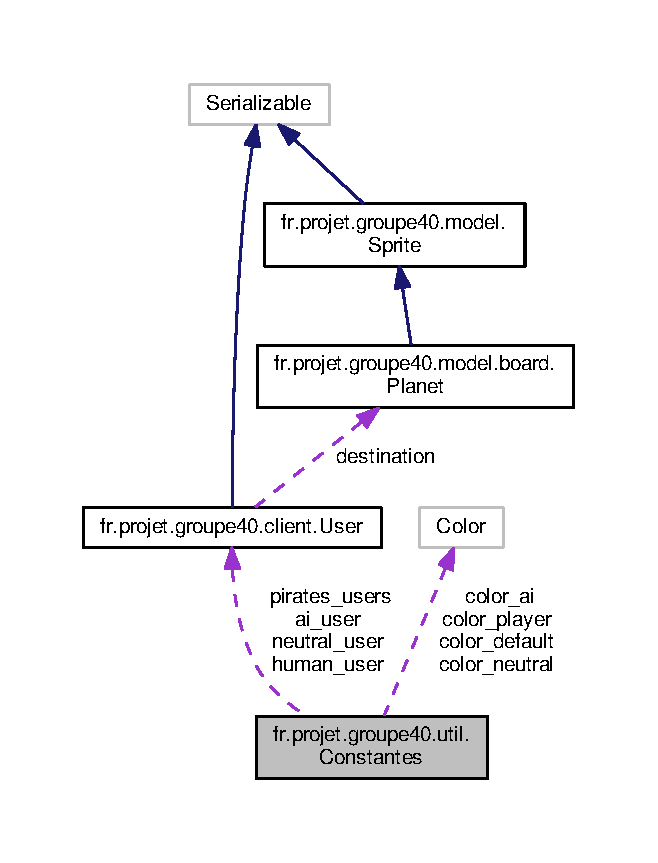
\includegraphics[width=316pt]{classfr_1_1projet_1_1groupe40_1_1util_1_1_constantes__coll__graph}
\end{center}
\end{figure}
\subsection*{Static Public Attributes}
\begin{DoxyCompactItemize}
\item 
static final String \hyperlink{classfr_1_1projet_1_1groupe40_1_1util_1_1_constantes_afa9920b6a2a81b225c1733c248b250ac}{name\+\_\+player2} = \char`\"{}IA 1\char`\"{}
\item 
static final double \hyperlink{classfr_1_1projet_1_1groupe40_1_1util_1_1_constantes_ac778f2c49769a86315ab7da9c80c6707}{PI} = 3.\+1415926535898
\item 
static final int \hyperlink{classfr_1_1projet_1_1groupe40_1_1util_1_1_constantes_a3aa832f1f1a73d73212e6c268993763f}{height} = 600
\item 
static final int \hyperlink{classfr_1_1projet_1_1groupe40_1_1util_1_1_constantes_a60fe40755417dae681b77621acfabebd}{width} = 800
\item 
static final double \hyperlink{classfr_1_1projet_1_1groupe40_1_1util_1_1_constantes_af7d767a7278f6e925c40373d39a0ee9c}{top\+\_\+margin\+\_\+size} = 50
\item 
static final double \hyperlink{classfr_1_1projet_1_1groupe40_1_1util_1_1_constantes_af515192a5a938c7cdc7aa1603c343918}{left\+\_\+margin\+\_\+size} = 50
\item 
static final double \hyperlink{classfr_1_1projet_1_1groupe40_1_1util_1_1_constantes_ad120e42952260b4b09723a1de78585b2}{bottom\+\_\+margin\+\_\+size} = 50
\item 
static final double \hyperlink{classfr_1_1projet_1_1groupe40_1_1util_1_1_constantes_a4b3510214fa2f517e6ee9efd95d6726b}{right\+\_\+margin\+\_\+size} = 50
\item 
static final int \hyperlink{classfr_1_1projet_1_1groupe40_1_1util_1_1_constantes_acd74074d64acf917e269065ba4cd5699}{nb\+\_\+planets\+\_\+tentatives} = 6
\item 
static final int \hyperlink{classfr_1_1projet_1_1groupe40_1_1util_1_1_constantes_a5af1ddef42b14e6be46461640d985ce6}{min\+\_\+numbers\+\_\+of\+\_\+planets} = 2
\item 
static final int \hyperlink{classfr_1_1projet_1_1groupe40_1_1util_1_1_constantes_a5e025fff7a0228bf0ba5e18e333e6e36}{minimal\+\_\+distance\+\_\+between\+\_\+planets} = 150
\item 
static final int \hyperlink{classfr_1_1projet_1_1groupe40_1_1util_1_1_constantes_af9918a7b68d5977d2b9d191df0ce4cb5}{nb\+\_\+squads} = 0
\item 
static final double \hyperlink{classfr_1_1projet_1_1groupe40_1_1util_1_1_constantes_ac4454baf5e684c8ef11e176811ca6539}{size\+\_\+squads} = 15.\+0
\item 
static final double \hyperlink{classfr_1_1projet_1_1groupe40_1_1util_1_1_constantes_ac93ce3978ee87e29e3200e70979bb319}{size\+\_\+minimal\+\_\+planets} = 4$\ast$15.\+0
\item 
static final double \hyperlink{classfr_1_1projet_1_1groupe40_1_1util_1_1_constantes_aac4e976050df9b797db436ae156e13d8}{size\+\_\+maximal\+\_\+planets} = 5$\ast$15.\+0
\item 
static final String \hyperlink{classfr_1_1projet_1_1groupe40_1_1util_1_1_constantes_a0ff9ae0397add21964b151cce6797fc9}{message\+\_\+game\+\_\+over} = \char`\"{}Vous avez perdu !\char`\"{}
\item 
static final double \hyperlink{classfr_1_1projet_1_1groupe40_1_1util_1_1_constantes_afc47053a18e107cf5725370809e30e9d}{min\+\_\+ship\+\_\+speed} = 3
\item 
static final double \hyperlink{classfr_1_1projet_1_1groupe40_1_1util_1_1_constantes_ac4190be1e9ede5f53c2c42328c53ed17}{min\+\_\+ship\+\_\+power} = 3
\item 
static final double \hyperlink{classfr_1_1projet_1_1groupe40_1_1util_1_1_constantes_ad6c52112c41d45f09b870da6c8183b7e}{min\+\_\+ship\+\_\+produce} = 1
\item 
static final double \hyperlink{classfr_1_1projet_1_1groupe40_1_1util_1_1_constantes_a308c37932d74f10d92367ccee5d6bc01}{max\+\_\+ship\+\_\+speed} = 5
\item 
static final double \hyperlink{classfr_1_1projet_1_1groupe40_1_1util_1_1_constantes_a2cf63e838bac482024489651ad5da853}{max\+\_\+ship\+\_\+power} = 7
\item 
static final double \hyperlink{classfr_1_1projet_1_1groupe40_1_1util_1_1_constantes_ac42829dfbb6a03d90d8445927dfb4458}{max\+\_\+ship\+\_\+produce} = 4
\item 
static final int \hyperlink{classfr_1_1projet_1_1groupe40_1_1util_1_1_constantes_a0569bd6ddee74127e4a8ec59890ea79a}{neutral} = 0
\item 
static final \hyperlink{classfr_1_1projet_1_1groupe40_1_1client_1_1_user}{User} \hyperlink{classfr_1_1projet_1_1groupe40_1_1util_1_1_constantes_af483735d1c6a1f063f02657d52d3bd4c}{neutral\+\_\+user} = new \hyperlink{classfr_1_1projet_1_1groupe40_1_1client_1_1_user}{User}(\hyperlink{classfr_1_1projet_1_1groupe40_1_1util_1_1_constantes_a0569bd6ddee74127e4a8ec59890ea79a}{neutral}, 0)
\item 
static final \hyperlink{classfr_1_1projet_1_1groupe40_1_1client_1_1_user}{User} \hyperlink{classfr_1_1projet_1_1groupe40_1_1util_1_1_constantes_a8445e21423d9e557d2cbdc37c99513ff}{ai\+\_\+user} = new \hyperlink{classfr_1_1projet_1_1groupe40_1_1client_1_1_user}{User}(ai, -\/1)
\item 
static final \hyperlink{classfr_1_1projet_1_1groupe40_1_1client_1_1_user}{User} \hyperlink{classfr_1_1projet_1_1groupe40_1_1util_1_1_constantes_a001dfc71bd19cf0985429b82bb445d7e}{pirates\+\_\+users} = new \hyperlink{classfr_1_1projet_1_1groupe40_1_1client_1_1_user}{User}(ai, -\/2)
\item 
static final \hyperlink{classfr_1_1projet_1_1groupe40_1_1client_1_1_user}{User} \hyperlink{classfr_1_1projet_1_1groupe40_1_1util_1_1_constantes_a44ea036556abe89e534f3fcb0ec18d73}{human\+\_\+user} = new \hyperlink{classfr_1_1projet_1_1groupe40_1_1client_1_1_user}{User}(player, 1)
\item 
static final long \hyperlink{classfr_1_1projet_1_1groupe40_1_1util_1_1_constantes_a4f2cf3e303ab9b072eb4611e55d054da}{ms\+\_\+per\+\_\+produce} = 1000
\item 
static final int \hyperlink{classfr_1_1projet_1_1groupe40_1_1util_1_1_constantes_a2bd65c5ef73d280d9f14b9ca2473d8f8}{max\+\_\+init\+Defense} = 15
\item 
static final int \hyperlink{classfr_1_1projet_1_1groupe40_1_1util_1_1_constantes_af4d6e6400edafa97c91c3f57aa734838}{min\+\_\+troups} = 1
\item 
static final int \hyperlink{classfr_1_1projet_1_1groupe40_1_1util_1_1_constantes_aba9d3c74d98acb0c7a8ee168ebae374d}{max\+\_\+troups} = 100
\item 
static final int \hyperlink{classfr_1_1projet_1_1groupe40_1_1util_1_1_constantes_ae0a76cc37f0fdb2ab7514c78f8c503dd}{size\+\_\+type\+Ships1} = 1
\item 
static final int \hyperlink{classfr_1_1projet_1_1groupe40_1_1util_1_1_constantes_a927632963a2d010a87055adaf0863633}{size\+\_\+type\+Ships2} = 5
\item 
static final int \hyperlink{classfr_1_1projet_1_1groupe40_1_1util_1_1_constantes_a1e26fc3e365203f88414786ce1741b57}{size\+\_\+type\+Ships3} = 25
\item 
static final int \hyperlink{classfr_1_1projet_1_1groupe40_1_1util_1_1_constantes_aced2a1f3350a1de856c19af6d8cbc518}{size\+\_\+type\+Ships4} = 50
\item 
static final Color \hyperlink{classfr_1_1projet_1_1groupe40_1_1util_1_1_constantes_ad5e5cffc8588cb22d0283158b1b349ee}{color\+\_\+neutral} = Color.\+D\+A\+R\+K\+G\+R\+AY
\item 
static final Color \hyperlink{classfr_1_1projet_1_1groupe40_1_1util_1_1_constantes_a7ddd842b46d4a546232331097d5280b2}{color\+\_\+player} = Color.\+L\+I\+G\+H\+T\+S\+E\+A\+G\+R\+E\+EN
\item 
static final Color \hyperlink{classfr_1_1projet_1_1groupe40_1_1util_1_1_constantes_af0b6b302d1e2765fdfb9718036385e3c}{color\+\_\+ai} = Color.\+R\+ED
\item 
static final Color \hyperlink{classfr_1_1projet_1_1groupe40_1_1util_1_1_constantes_a846d5c141ee33283dcd1854275428a91}{color\+\_\+default} = Color.\+W\+H\+I\+TE
\item 
static final String \hyperlink{classfr_1_1projet_1_1groupe40_1_1util_1_1_constantes_adc35eacdfaca48bcc97da027ec46d0db}{path\+\_\+save} = \char`\"{}\char`\"{}
\item 
static final String \hyperlink{classfr_1_1projet_1_1groupe40_1_1util_1_1_constantes_afe0c37178c229c3881bf835bb16c45d8}{path\+\_\+img\+\_\+planets} = \char`\"{}/resources/images/square.\+png\char`\"{}
\item 
static final String \hyperlink{classfr_1_1projet_1_1groupe40_1_1util_1_1_constantes_a8b2368e6628d7a454badd705097242cd}{path\+\_\+img\+\_\+ships} = \char`\"{}/resources/images/alien.\+png\char`\"{}
\item 
static final String \hyperlink{classfr_1_1projet_1_1groupe40_1_1util_1_1_constantes_ac6bcb73d6876b90d9f1ffd17f0591ce5}{path\+\_\+img\+\_\+background} = \char`\"{}/resources/images/background.\+jpg\char`\"{}
\item 
static final String \hyperlink{classfr_1_1projet_1_1groupe40_1_1util_1_1_constantes_ae140c3640e847487363a59291d33fd8c}{path\+\_\+img\+\_\+round\+\_\+planets} = null
\item 
static final String \hyperlink{classfr_1_1projet_1_1groupe40_1_1util_1_1_constantes_ab2e1584ef3a7dec746947bc3797856c7}{path\+\_\+sound\+\_\+explosion} = \char`\"{}/resources/sounds/Engine.\+mp4\char`\"{}
\item 
static final String \hyperlink{classfr_1_1projet_1_1groupe40_1_1util_1_1_constantes_a1c4f9406019ba0070d7e8ac01c8da8c2}{path\+\_\+sound\+\_\+aa} = \char`\"{}/resources/sounds/aa.\+mp4\char`\"{}
\item 
static final int \hyperlink{classfr_1_1projet_1_1groupe40_1_1util_1_1_constantes_a62db33b20e7538cc4db4de9aa26a9188}{error\+\_\+greater\+\_\+x} = 2
\item 
static final int \hyperlink{classfr_1_1projet_1_1groupe40_1_1util_1_1_constantes_aba6dabe9122cbaf1e580700e1583c39d}{error\+\_\+greater\+\_\+y} = 1
\item 
static final int \hyperlink{classfr_1_1projet_1_1groupe40_1_1util_1_1_constantes_afc47dab9026574f1397d88cefeb47c6b}{error\+\_\+lower\+\_\+x} = -\/1
\item 
static final int \hyperlink{classfr_1_1projet_1_1groupe40_1_1util_1_1_constantes_acf4616f5c5c27a22df9a44bb0142c8ad}{error\+\_\+lower\+\_\+y} = -\/2
\item 
static final boolean \hyperlink{classfr_1_1projet_1_1groupe40_1_1util_1_1_constantes_ab1177197da83e8d896e32796e50799fe}{D\+E\+B\+UG} = false
\item 
static final boolean \hyperlink{classfr_1_1projet_1_1groupe40_1_1util_1_1_constantes_a58a90e1be21154f908e85f3f302a7adf}{D\+E\+B\+U\+G\+\_\+\+T\+R\+O\+U\+PS} = false
\item 
static final boolean \hyperlink{classfr_1_1projet_1_1groupe40_1_1util_1_1_constantes_a68d7ea5b02ac2fa94f2edabef7bd7793}{limit\+\_\+ai\+\_\+squads\+\_\+number} = true
\item 
static final int \hyperlink{classfr_1_1projet_1_1groupe40_1_1util_1_1_constantes_a2682082f9f3e56728af6066427a63a4a}{max\+\_\+squads\+\_\+for\+\_\+ai} = 2
\end{DoxyCompactItemize}


\subsection{Member Data Documentation}
\mbox{\Hypertarget{classfr_1_1projet_1_1groupe40_1_1util_1_1_constantes_a8445e21423d9e557d2cbdc37c99513ff}\label{classfr_1_1projet_1_1groupe40_1_1util_1_1_constantes_a8445e21423d9e557d2cbdc37c99513ff}} 
\index{fr\+::projet\+::groupe40\+::util\+::\+Constantes@{fr\+::projet\+::groupe40\+::util\+::\+Constantes}!ai\+\_\+user@{ai\+\_\+user}}
\index{ai\+\_\+user@{ai\+\_\+user}!fr\+::projet\+::groupe40\+::util\+::\+Constantes@{fr\+::projet\+::groupe40\+::util\+::\+Constantes}}
\subsubsection{\texorpdfstring{ai\+\_\+user}{ai\_user}}
{\footnotesize\ttfamily final \hyperlink{classfr_1_1projet_1_1groupe40_1_1client_1_1_user}{User} fr.\+projet.\+groupe40.\+util.\+Constantes.\+ai\+\_\+user = new \hyperlink{classfr_1_1projet_1_1groupe40_1_1client_1_1_user}{User}(ai, -\/1)\hspace{0.3cm}{\ttfamily [static]}}

\mbox{\Hypertarget{classfr_1_1projet_1_1groupe40_1_1util_1_1_constantes_ad120e42952260b4b09723a1de78585b2}\label{classfr_1_1projet_1_1groupe40_1_1util_1_1_constantes_ad120e42952260b4b09723a1de78585b2}} 
\index{fr\+::projet\+::groupe40\+::util\+::\+Constantes@{fr\+::projet\+::groupe40\+::util\+::\+Constantes}!bottom\+\_\+margin\+\_\+size@{bottom\+\_\+margin\+\_\+size}}
\index{bottom\+\_\+margin\+\_\+size@{bottom\+\_\+margin\+\_\+size}!fr\+::projet\+::groupe40\+::util\+::\+Constantes@{fr\+::projet\+::groupe40\+::util\+::\+Constantes}}
\subsubsection{\texorpdfstring{bottom\+\_\+margin\+\_\+size}{bottom\_margin\_size}}
{\footnotesize\ttfamily final double fr.\+projet.\+groupe40.\+util.\+Constantes.\+bottom\+\_\+margin\+\_\+size = 50\hspace{0.3cm}{\ttfamily [static]}}

\mbox{\Hypertarget{classfr_1_1projet_1_1groupe40_1_1util_1_1_constantes_af0b6b302d1e2765fdfb9718036385e3c}\label{classfr_1_1projet_1_1groupe40_1_1util_1_1_constantes_af0b6b302d1e2765fdfb9718036385e3c}} 
\index{fr\+::projet\+::groupe40\+::util\+::\+Constantes@{fr\+::projet\+::groupe40\+::util\+::\+Constantes}!color\+\_\+ai@{color\+\_\+ai}}
\index{color\+\_\+ai@{color\+\_\+ai}!fr\+::projet\+::groupe40\+::util\+::\+Constantes@{fr\+::projet\+::groupe40\+::util\+::\+Constantes}}
\subsubsection{\texorpdfstring{color\+\_\+ai}{color\_ai}}
{\footnotesize\ttfamily final Color fr.\+projet.\+groupe40.\+util.\+Constantes.\+color\+\_\+ai = Color.\+R\+ED\hspace{0.3cm}{\ttfamily [static]}}

\mbox{\Hypertarget{classfr_1_1projet_1_1groupe40_1_1util_1_1_constantes_a846d5c141ee33283dcd1854275428a91}\label{classfr_1_1projet_1_1groupe40_1_1util_1_1_constantes_a846d5c141ee33283dcd1854275428a91}} 
\index{fr\+::projet\+::groupe40\+::util\+::\+Constantes@{fr\+::projet\+::groupe40\+::util\+::\+Constantes}!color\+\_\+default@{color\+\_\+default}}
\index{color\+\_\+default@{color\+\_\+default}!fr\+::projet\+::groupe40\+::util\+::\+Constantes@{fr\+::projet\+::groupe40\+::util\+::\+Constantes}}
\subsubsection{\texorpdfstring{color\+\_\+default}{color\_default}}
{\footnotesize\ttfamily final Color fr.\+projet.\+groupe40.\+util.\+Constantes.\+color\+\_\+default = Color.\+W\+H\+I\+TE\hspace{0.3cm}{\ttfamily [static]}}

\mbox{\Hypertarget{classfr_1_1projet_1_1groupe40_1_1util_1_1_constantes_ad5e5cffc8588cb22d0283158b1b349ee}\label{classfr_1_1projet_1_1groupe40_1_1util_1_1_constantes_ad5e5cffc8588cb22d0283158b1b349ee}} 
\index{fr\+::projet\+::groupe40\+::util\+::\+Constantes@{fr\+::projet\+::groupe40\+::util\+::\+Constantes}!color\+\_\+neutral@{color\+\_\+neutral}}
\index{color\+\_\+neutral@{color\+\_\+neutral}!fr\+::projet\+::groupe40\+::util\+::\+Constantes@{fr\+::projet\+::groupe40\+::util\+::\+Constantes}}
\subsubsection{\texorpdfstring{color\+\_\+neutral}{color\_neutral}}
{\footnotesize\ttfamily final Color fr.\+projet.\+groupe40.\+util.\+Constantes.\+color\+\_\+neutral = Color.\+D\+A\+R\+K\+G\+R\+AY\hspace{0.3cm}{\ttfamily [static]}}

Color \mbox{\Hypertarget{classfr_1_1projet_1_1groupe40_1_1util_1_1_constantes_a7ddd842b46d4a546232331097d5280b2}\label{classfr_1_1projet_1_1groupe40_1_1util_1_1_constantes_a7ddd842b46d4a546232331097d5280b2}} 
\index{fr\+::projet\+::groupe40\+::util\+::\+Constantes@{fr\+::projet\+::groupe40\+::util\+::\+Constantes}!color\+\_\+player@{color\+\_\+player}}
\index{color\+\_\+player@{color\+\_\+player}!fr\+::projet\+::groupe40\+::util\+::\+Constantes@{fr\+::projet\+::groupe40\+::util\+::\+Constantes}}
\subsubsection{\texorpdfstring{color\+\_\+player}{color\_player}}
{\footnotesize\ttfamily final Color fr.\+projet.\+groupe40.\+util.\+Constantes.\+color\+\_\+player = Color.\+L\+I\+G\+H\+T\+S\+E\+A\+G\+R\+E\+EN\hspace{0.3cm}{\ttfamily [static]}}

\mbox{\Hypertarget{classfr_1_1projet_1_1groupe40_1_1util_1_1_constantes_ab1177197da83e8d896e32796e50799fe}\label{classfr_1_1projet_1_1groupe40_1_1util_1_1_constantes_ab1177197da83e8d896e32796e50799fe}} 
\index{fr\+::projet\+::groupe40\+::util\+::\+Constantes@{fr\+::projet\+::groupe40\+::util\+::\+Constantes}!D\+E\+B\+UG@{D\+E\+B\+UG}}
\index{D\+E\+B\+UG@{D\+E\+B\+UG}!fr\+::projet\+::groupe40\+::util\+::\+Constantes@{fr\+::projet\+::groupe40\+::util\+::\+Constantes}}
\subsubsection{\texorpdfstring{D\+E\+B\+UG}{DEBUG}}
{\footnotesize\ttfamily final boolean fr.\+projet.\+groupe40.\+util.\+Constantes.\+D\+E\+B\+UG = false\hspace{0.3cm}{\ttfamily [static]}}

\mbox{\Hypertarget{classfr_1_1projet_1_1groupe40_1_1util_1_1_constantes_a58a90e1be21154f908e85f3f302a7adf}\label{classfr_1_1projet_1_1groupe40_1_1util_1_1_constantes_a58a90e1be21154f908e85f3f302a7adf}} 
\index{fr\+::projet\+::groupe40\+::util\+::\+Constantes@{fr\+::projet\+::groupe40\+::util\+::\+Constantes}!D\+E\+B\+U\+G\+\_\+\+T\+R\+O\+U\+PS@{D\+E\+B\+U\+G\+\_\+\+T\+R\+O\+U\+PS}}
\index{D\+E\+B\+U\+G\+\_\+\+T\+R\+O\+U\+PS@{D\+E\+B\+U\+G\+\_\+\+T\+R\+O\+U\+PS}!fr\+::projet\+::groupe40\+::util\+::\+Constantes@{fr\+::projet\+::groupe40\+::util\+::\+Constantes}}
\subsubsection{\texorpdfstring{D\+E\+B\+U\+G\+\_\+\+T\+R\+O\+U\+PS}{DEBUG\_TROUPS}}
{\footnotesize\ttfamily final boolean fr.\+projet.\+groupe40.\+util.\+Constantes.\+D\+E\+B\+U\+G\+\_\+\+T\+R\+O\+U\+PS = false\hspace{0.3cm}{\ttfamily [static]}}

\mbox{\Hypertarget{classfr_1_1projet_1_1groupe40_1_1util_1_1_constantes_a62db33b20e7538cc4db4de9aa26a9188}\label{classfr_1_1projet_1_1groupe40_1_1util_1_1_constantes_a62db33b20e7538cc4db4de9aa26a9188}} 
\index{fr\+::projet\+::groupe40\+::util\+::\+Constantes@{fr\+::projet\+::groupe40\+::util\+::\+Constantes}!error\+\_\+greater\+\_\+x@{error\+\_\+greater\+\_\+x}}
\index{error\+\_\+greater\+\_\+x@{error\+\_\+greater\+\_\+x}!fr\+::projet\+::groupe40\+::util\+::\+Constantes@{fr\+::projet\+::groupe40\+::util\+::\+Constantes}}
\subsubsection{\texorpdfstring{error\+\_\+greater\+\_\+x}{error\_greater\_x}}
{\footnotesize\ttfamily final int fr.\+projet.\+groupe40.\+util.\+Constantes.\+error\+\_\+greater\+\_\+x = 2\hspace{0.3cm}{\ttfamily [static]}}

Error \& Debugging \mbox{\Hypertarget{classfr_1_1projet_1_1groupe40_1_1util_1_1_constantes_aba6dabe9122cbaf1e580700e1583c39d}\label{classfr_1_1projet_1_1groupe40_1_1util_1_1_constantes_aba6dabe9122cbaf1e580700e1583c39d}} 
\index{fr\+::projet\+::groupe40\+::util\+::\+Constantes@{fr\+::projet\+::groupe40\+::util\+::\+Constantes}!error\+\_\+greater\+\_\+y@{error\+\_\+greater\+\_\+y}}
\index{error\+\_\+greater\+\_\+y@{error\+\_\+greater\+\_\+y}!fr\+::projet\+::groupe40\+::util\+::\+Constantes@{fr\+::projet\+::groupe40\+::util\+::\+Constantes}}
\subsubsection{\texorpdfstring{error\+\_\+greater\+\_\+y}{error\_greater\_y}}
{\footnotesize\ttfamily final int fr.\+projet.\+groupe40.\+util.\+Constantes.\+error\+\_\+greater\+\_\+y = 1\hspace{0.3cm}{\ttfamily [static]}}

\mbox{\Hypertarget{classfr_1_1projet_1_1groupe40_1_1util_1_1_constantes_afc47dab9026574f1397d88cefeb47c6b}\label{classfr_1_1projet_1_1groupe40_1_1util_1_1_constantes_afc47dab9026574f1397d88cefeb47c6b}} 
\index{fr\+::projet\+::groupe40\+::util\+::\+Constantes@{fr\+::projet\+::groupe40\+::util\+::\+Constantes}!error\+\_\+lower\+\_\+x@{error\+\_\+lower\+\_\+x}}
\index{error\+\_\+lower\+\_\+x@{error\+\_\+lower\+\_\+x}!fr\+::projet\+::groupe40\+::util\+::\+Constantes@{fr\+::projet\+::groupe40\+::util\+::\+Constantes}}
\subsubsection{\texorpdfstring{error\+\_\+lower\+\_\+x}{error\_lower\_x}}
{\footnotesize\ttfamily final int fr.\+projet.\+groupe40.\+util.\+Constantes.\+error\+\_\+lower\+\_\+x = -\/1\hspace{0.3cm}{\ttfamily [static]}}

\mbox{\Hypertarget{classfr_1_1projet_1_1groupe40_1_1util_1_1_constantes_acf4616f5c5c27a22df9a44bb0142c8ad}\label{classfr_1_1projet_1_1groupe40_1_1util_1_1_constantes_acf4616f5c5c27a22df9a44bb0142c8ad}} 
\index{fr\+::projet\+::groupe40\+::util\+::\+Constantes@{fr\+::projet\+::groupe40\+::util\+::\+Constantes}!error\+\_\+lower\+\_\+y@{error\+\_\+lower\+\_\+y}}
\index{error\+\_\+lower\+\_\+y@{error\+\_\+lower\+\_\+y}!fr\+::projet\+::groupe40\+::util\+::\+Constantes@{fr\+::projet\+::groupe40\+::util\+::\+Constantes}}
\subsubsection{\texorpdfstring{error\+\_\+lower\+\_\+y}{error\_lower\_y}}
{\footnotesize\ttfamily final int fr.\+projet.\+groupe40.\+util.\+Constantes.\+error\+\_\+lower\+\_\+y = -\/2\hspace{0.3cm}{\ttfamily [static]}}

\mbox{\Hypertarget{classfr_1_1projet_1_1groupe40_1_1util_1_1_constantes_a3aa832f1f1a73d73212e6c268993763f}\label{classfr_1_1projet_1_1groupe40_1_1util_1_1_constantes_a3aa832f1f1a73d73212e6c268993763f}} 
\index{fr\+::projet\+::groupe40\+::util\+::\+Constantes@{fr\+::projet\+::groupe40\+::util\+::\+Constantes}!height@{height}}
\index{height@{height}!fr\+::projet\+::groupe40\+::util\+::\+Constantes@{fr\+::projet\+::groupe40\+::util\+::\+Constantes}}
\subsubsection{\texorpdfstring{height}{height}}
{\footnotesize\ttfamily final int fr.\+projet.\+groupe40.\+util.\+Constantes.\+height = 600\hspace{0.3cm}{\ttfamily [static]}}

Window Parameters \mbox{\Hypertarget{classfr_1_1projet_1_1groupe40_1_1util_1_1_constantes_a44ea036556abe89e534f3fcb0ec18d73}\label{classfr_1_1projet_1_1groupe40_1_1util_1_1_constantes_a44ea036556abe89e534f3fcb0ec18d73}} 
\index{fr\+::projet\+::groupe40\+::util\+::\+Constantes@{fr\+::projet\+::groupe40\+::util\+::\+Constantes}!human\+\_\+user@{human\+\_\+user}}
\index{human\+\_\+user@{human\+\_\+user}!fr\+::projet\+::groupe40\+::util\+::\+Constantes@{fr\+::projet\+::groupe40\+::util\+::\+Constantes}}
\subsubsection{\texorpdfstring{human\+\_\+user}{human\_user}}
{\footnotesize\ttfamily final \hyperlink{classfr_1_1projet_1_1groupe40_1_1client_1_1_user}{User} fr.\+projet.\+groupe40.\+util.\+Constantes.\+human\+\_\+user = new \hyperlink{classfr_1_1projet_1_1groupe40_1_1client_1_1_user}{User}(player, 1)\hspace{0.3cm}{\ttfamily [static]}}

\mbox{\Hypertarget{classfr_1_1projet_1_1groupe40_1_1util_1_1_constantes_af515192a5a938c7cdc7aa1603c343918}\label{classfr_1_1projet_1_1groupe40_1_1util_1_1_constantes_af515192a5a938c7cdc7aa1603c343918}} 
\index{fr\+::projet\+::groupe40\+::util\+::\+Constantes@{fr\+::projet\+::groupe40\+::util\+::\+Constantes}!left\+\_\+margin\+\_\+size@{left\+\_\+margin\+\_\+size}}
\index{left\+\_\+margin\+\_\+size@{left\+\_\+margin\+\_\+size}!fr\+::projet\+::groupe40\+::util\+::\+Constantes@{fr\+::projet\+::groupe40\+::util\+::\+Constantes}}
\subsubsection{\texorpdfstring{left\+\_\+margin\+\_\+size}{left\_margin\_size}}
{\footnotesize\ttfamily final double fr.\+projet.\+groupe40.\+util.\+Constantes.\+left\+\_\+margin\+\_\+size = 50\hspace{0.3cm}{\ttfamily [static]}}

\mbox{\Hypertarget{classfr_1_1projet_1_1groupe40_1_1util_1_1_constantes_a68d7ea5b02ac2fa94f2edabef7bd7793}\label{classfr_1_1projet_1_1groupe40_1_1util_1_1_constantes_a68d7ea5b02ac2fa94f2edabef7bd7793}} 
\index{fr\+::projet\+::groupe40\+::util\+::\+Constantes@{fr\+::projet\+::groupe40\+::util\+::\+Constantes}!limit\+\_\+ai\+\_\+squads\+\_\+number@{limit\+\_\+ai\+\_\+squads\+\_\+number}}
\index{limit\+\_\+ai\+\_\+squads\+\_\+number@{limit\+\_\+ai\+\_\+squads\+\_\+number}!fr\+::projet\+::groupe40\+::util\+::\+Constantes@{fr\+::projet\+::groupe40\+::util\+::\+Constantes}}
\subsubsection{\texorpdfstring{limit\+\_\+ai\+\_\+squads\+\_\+number}{limit\_ai\_squads\_number}}
{\footnotesize\ttfamily final boolean fr.\+projet.\+groupe40.\+util.\+Constantes.\+limit\+\_\+ai\+\_\+squads\+\_\+number = true\hspace{0.3cm}{\ttfamily [static]}}

AI Config \mbox{\Hypertarget{classfr_1_1projet_1_1groupe40_1_1util_1_1_constantes_a2bd65c5ef73d280d9f14b9ca2473d8f8}\label{classfr_1_1projet_1_1groupe40_1_1util_1_1_constantes_a2bd65c5ef73d280d9f14b9ca2473d8f8}} 
\index{fr\+::projet\+::groupe40\+::util\+::\+Constantes@{fr\+::projet\+::groupe40\+::util\+::\+Constantes}!max\+\_\+init\+Defense@{max\+\_\+init\+Defense}}
\index{max\+\_\+init\+Defense@{max\+\_\+init\+Defense}!fr\+::projet\+::groupe40\+::util\+::\+Constantes@{fr\+::projet\+::groupe40\+::util\+::\+Constantes}}
\subsubsection{\texorpdfstring{max\+\_\+init\+Defense}{max\_initDefense}}
{\footnotesize\ttfamily final int fr.\+projet.\+groupe40.\+util.\+Constantes.\+max\+\_\+init\+Defense = 15\hspace{0.3cm}{\ttfamily [static]}}

\mbox{\Hypertarget{classfr_1_1projet_1_1groupe40_1_1util_1_1_constantes_a2cf63e838bac482024489651ad5da853}\label{classfr_1_1projet_1_1groupe40_1_1util_1_1_constantes_a2cf63e838bac482024489651ad5da853}} 
\index{fr\+::projet\+::groupe40\+::util\+::\+Constantes@{fr\+::projet\+::groupe40\+::util\+::\+Constantes}!max\+\_\+ship\+\_\+power@{max\+\_\+ship\+\_\+power}}
\index{max\+\_\+ship\+\_\+power@{max\+\_\+ship\+\_\+power}!fr\+::projet\+::groupe40\+::util\+::\+Constantes@{fr\+::projet\+::groupe40\+::util\+::\+Constantes}}
\subsubsection{\texorpdfstring{max\+\_\+ship\+\_\+power}{max\_ship\_power}}
{\footnotesize\ttfamily final double fr.\+projet.\+groupe40.\+util.\+Constantes.\+max\+\_\+ship\+\_\+power = 7\hspace{0.3cm}{\ttfamily [static]}}

\mbox{\Hypertarget{classfr_1_1projet_1_1groupe40_1_1util_1_1_constantes_ac42829dfbb6a03d90d8445927dfb4458}\label{classfr_1_1projet_1_1groupe40_1_1util_1_1_constantes_ac42829dfbb6a03d90d8445927dfb4458}} 
\index{fr\+::projet\+::groupe40\+::util\+::\+Constantes@{fr\+::projet\+::groupe40\+::util\+::\+Constantes}!max\+\_\+ship\+\_\+produce@{max\+\_\+ship\+\_\+produce}}
\index{max\+\_\+ship\+\_\+produce@{max\+\_\+ship\+\_\+produce}!fr\+::projet\+::groupe40\+::util\+::\+Constantes@{fr\+::projet\+::groupe40\+::util\+::\+Constantes}}
\subsubsection{\texorpdfstring{max\+\_\+ship\+\_\+produce}{max\_ship\_produce}}
{\footnotesize\ttfamily final double fr.\+projet.\+groupe40.\+util.\+Constantes.\+max\+\_\+ship\+\_\+produce = 4\hspace{0.3cm}{\ttfamily [static]}}

\mbox{\Hypertarget{classfr_1_1projet_1_1groupe40_1_1util_1_1_constantes_a308c37932d74f10d92367ccee5d6bc01}\label{classfr_1_1projet_1_1groupe40_1_1util_1_1_constantes_a308c37932d74f10d92367ccee5d6bc01}} 
\index{fr\+::projet\+::groupe40\+::util\+::\+Constantes@{fr\+::projet\+::groupe40\+::util\+::\+Constantes}!max\+\_\+ship\+\_\+speed@{max\+\_\+ship\+\_\+speed}}
\index{max\+\_\+ship\+\_\+speed@{max\+\_\+ship\+\_\+speed}!fr\+::projet\+::groupe40\+::util\+::\+Constantes@{fr\+::projet\+::groupe40\+::util\+::\+Constantes}}
\subsubsection{\texorpdfstring{max\+\_\+ship\+\_\+speed}{max\_ship\_speed}}
{\footnotesize\ttfamily final double fr.\+projet.\+groupe40.\+util.\+Constantes.\+max\+\_\+ship\+\_\+speed = 5\hspace{0.3cm}{\ttfamily [static]}}

\mbox{\Hypertarget{classfr_1_1projet_1_1groupe40_1_1util_1_1_constantes_a2682082f9f3e56728af6066427a63a4a}\label{classfr_1_1projet_1_1groupe40_1_1util_1_1_constantes_a2682082f9f3e56728af6066427a63a4a}} 
\index{fr\+::projet\+::groupe40\+::util\+::\+Constantes@{fr\+::projet\+::groupe40\+::util\+::\+Constantes}!max\+\_\+squads\+\_\+for\+\_\+ai@{max\+\_\+squads\+\_\+for\+\_\+ai}}
\index{max\+\_\+squads\+\_\+for\+\_\+ai@{max\+\_\+squads\+\_\+for\+\_\+ai}!fr\+::projet\+::groupe40\+::util\+::\+Constantes@{fr\+::projet\+::groupe40\+::util\+::\+Constantes}}
\subsubsection{\texorpdfstring{max\+\_\+squads\+\_\+for\+\_\+ai}{max\_squads\_for\_ai}}
{\footnotesize\ttfamily final int fr.\+projet.\+groupe40.\+util.\+Constantes.\+max\+\_\+squads\+\_\+for\+\_\+ai = 2\hspace{0.3cm}{\ttfamily [static]}}

\mbox{\Hypertarget{classfr_1_1projet_1_1groupe40_1_1util_1_1_constantes_aba9d3c74d98acb0c7a8ee168ebae374d}\label{classfr_1_1projet_1_1groupe40_1_1util_1_1_constantes_aba9d3c74d98acb0c7a8ee168ebae374d}} 
\index{fr\+::projet\+::groupe40\+::util\+::\+Constantes@{fr\+::projet\+::groupe40\+::util\+::\+Constantes}!max\+\_\+troups@{max\+\_\+troups}}
\index{max\+\_\+troups@{max\+\_\+troups}!fr\+::projet\+::groupe40\+::util\+::\+Constantes@{fr\+::projet\+::groupe40\+::util\+::\+Constantes}}
\subsubsection{\texorpdfstring{max\+\_\+troups}{max\_troups}}
{\footnotesize\ttfamily final int fr.\+projet.\+groupe40.\+util.\+Constantes.\+max\+\_\+troups = 100\hspace{0.3cm}{\ttfamily [static]}}

\mbox{\Hypertarget{classfr_1_1projet_1_1groupe40_1_1util_1_1_constantes_a0ff9ae0397add21964b151cce6797fc9}\label{classfr_1_1projet_1_1groupe40_1_1util_1_1_constantes_a0ff9ae0397add21964b151cce6797fc9}} 
\index{fr\+::projet\+::groupe40\+::util\+::\+Constantes@{fr\+::projet\+::groupe40\+::util\+::\+Constantes}!message\+\_\+game\+\_\+over@{message\+\_\+game\+\_\+over}}
\index{message\+\_\+game\+\_\+over@{message\+\_\+game\+\_\+over}!fr\+::projet\+::groupe40\+::util\+::\+Constantes@{fr\+::projet\+::groupe40\+::util\+::\+Constantes}}
\subsubsection{\texorpdfstring{message\+\_\+game\+\_\+over}{message\_game\_over}}
{\footnotesize\ttfamily final String fr.\+projet.\+groupe40.\+util.\+Constantes.\+message\+\_\+game\+\_\+over = \char`\"{}Vous avez perdu !\char`\"{}\hspace{0.3cm}{\ttfamily [static]}}

\mbox{\Hypertarget{classfr_1_1projet_1_1groupe40_1_1util_1_1_constantes_a5af1ddef42b14e6be46461640d985ce6}\label{classfr_1_1projet_1_1groupe40_1_1util_1_1_constantes_a5af1ddef42b14e6be46461640d985ce6}} 
\index{fr\+::projet\+::groupe40\+::util\+::\+Constantes@{fr\+::projet\+::groupe40\+::util\+::\+Constantes}!min\+\_\+numbers\+\_\+of\+\_\+planets@{min\+\_\+numbers\+\_\+of\+\_\+planets}}
\index{min\+\_\+numbers\+\_\+of\+\_\+planets@{min\+\_\+numbers\+\_\+of\+\_\+planets}!fr\+::projet\+::groupe40\+::util\+::\+Constantes@{fr\+::projet\+::groupe40\+::util\+::\+Constantes}}
\subsubsection{\texorpdfstring{min\+\_\+numbers\+\_\+of\+\_\+planets}{min\_numbers\_of\_planets}}
{\footnotesize\ttfamily final int fr.\+projet.\+groupe40.\+util.\+Constantes.\+min\+\_\+numbers\+\_\+of\+\_\+planets = 2\hspace{0.3cm}{\ttfamily [static]}}

\mbox{\Hypertarget{classfr_1_1projet_1_1groupe40_1_1util_1_1_constantes_ac4190be1e9ede5f53c2c42328c53ed17}\label{classfr_1_1projet_1_1groupe40_1_1util_1_1_constantes_ac4190be1e9ede5f53c2c42328c53ed17}} 
\index{fr\+::projet\+::groupe40\+::util\+::\+Constantes@{fr\+::projet\+::groupe40\+::util\+::\+Constantes}!min\+\_\+ship\+\_\+power@{min\+\_\+ship\+\_\+power}}
\index{min\+\_\+ship\+\_\+power@{min\+\_\+ship\+\_\+power}!fr\+::projet\+::groupe40\+::util\+::\+Constantes@{fr\+::projet\+::groupe40\+::util\+::\+Constantes}}
\subsubsection{\texorpdfstring{min\+\_\+ship\+\_\+power}{min\_ship\_power}}
{\footnotesize\ttfamily final double fr.\+projet.\+groupe40.\+util.\+Constantes.\+min\+\_\+ship\+\_\+power = 3\hspace{0.3cm}{\ttfamily [static]}}

\mbox{\Hypertarget{classfr_1_1projet_1_1groupe40_1_1util_1_1_constantes_ad6c52112c41d45f09b870da6c8183b7e}\label{classfr_1_1projet_1_1groupe40_1_1util_1_1_constantes_ad6c52112c41d45f09b870da6c8183b7e}} 
\index{fr\+::projet\+::groupe40\+::util\+::\+Constantes@{fr\+::projet\+::groupe40\+::util\+::\+Constantes}!min\+\_\+ship\+\_\+produce@{min\+\_\+ship\+\_\+produce}}
\index{min\+\_\+ship\+\_\+produce@{min\+\_\+ship\+\_\+produce}!fr\+::projet\+::groupe40\+::util\+::\+Constantes@{fr\+::projet\+::groupe40\+::util\+::\+Constantes}}
\subsubsection{\texorpdfstring{min\+\_\+ship\+\_\+produce}{min\_ship\_produce}}
{\footnotesize\ttfamily final double fr.\+projet.\+groupe40.\+util.\+Constantes.\+min\+\_\+ship\+\_\+produce = 1\hspace{0.3cm}{\ttfamily [static]}}

\mbox{\Hypertarget{classfr_1_1projet_1_1groupe40_1_1util_1_1_constantes_afc47053a18e107cf5725370809e30e9d}\label{classfr_1_1projet_1_1groupe40_1_1util_1_1_constantes_afc47053a18e107cf5725370809e30e9d}} 
\index{fr\+::projet\+::groupe40\+::util\+::\+Constantes@{fr\+::projet\+::groupe40\+::util\+::\+Constantes}!min\+\_\+ship\+\_\+speed@{min\+\_\+ship\+\_\+speed}}
\index{min\+\_\+ship\+\_\+speed@{min\+\_\+ship\+\_\+speed}!fr\+::projet\+::groupe40\+::util\+::\+Constantes@{fr\+::projet\+::groupe40\+::util\+::\+Constantes}}
\subsubsection{\texorpdfstring{min\+\_\+ship\+\_\+speed}{min\_ship\_speed}}
{\footnotesize\ttfamily final double fr.\+projet.\+groupe40.\+util.\+Constantes.\+min\+\_\+ship\+\_\+speed = 3\hspace{0.3cm}{\ttfamily [static]}}

Ships Options \mbox{\Hypertarget{classfr_1_1projet_1_1groupe40_1_1util_1_1_constantes_af4d6e6400edafa97c91c3f57aa734838}\label{classfr_1_1projet_1_1groupe40_1_1util_1_1_constantes_af4d6e6400edafa97c91c3f57aa734838}} 
\index{fr\+::projet\+::groupe40\+::util\+::\+Constantes@{fr\+::projet\+::groupe40\+::util\+::\+Constantes}!min\+\_\+troups@{min\+\_\+troups}}
\index{min\+\_\+troups@{min\+\_\+troups}!fr\+::projet\+::groupe40\+::util\+::\+Constantes@{fr\+::projet\+::groupe40\+::util\+::\+Constantes}}
\subsubsection{\texorpdfstring{min\+\_\+troups}{min\_troups}}
{\footnotesize\ttfamily final int fr.\+projet.\+groupe40.\+util.\+Constantes.\+min\+\_\+troups = 1\hspace{0.3cm}{\ttfamily [static]}}

\mbox{\Hypertarget{classfr_1_1projet_1_1groupe40_1_1util_1_1_constantes_a5e025fff7a0228bf0ba5e18e333e6e36}\label{classfr_1_1projet_1_1groupe40_1_1util_1_1_constantes_a5e025fff7a0228bf0ba5e18e333e6e36}} 
\index{fr\+::projet\+::groupe40\+::util\+::\+Constantes@{fr\+::projet\+::groupe40\+::util\+::\+Constantes}!minimal\+\_\+distance\+\_\+between\+\_\+planets@{minimal\+\_\+distance\+\_\+between\+\_\+planets}}
\index{minimal\+\_\+distance\+\_\+between\+\_\+planets@{minimal\+\_\+distance\+\_\+between\+\_\+planets}!fr\+::projet\+::groupe40\+::util\+::\+Constantes@{fr\+::projet\+::groupe40\+::util\+::\+Constantes}}
\subsubsection{\texorpdfstring{minimal\+\_\+distance\+\_\+between\+\_\+planets}{minimal\_distance\_between\_planets}}
{\footnotesize\ttfamily final int fr.\+projet.\+groupe40.\+util.\+Constantes.\+minimal\+\_\+distance\+\_\+between\+\_\+planets = 150\hspace{0.3cm}{\ttfamily [static]}}

\mbox{\Hypertarget{classfr_1_1projet_1_1groupe40_1_1util_1_1_constantes_a4f2cf3e303ab9b072eb4611e55d054da}\label{classfr_1_1projet_1_1groupe40_1_1util_1_1_constantes_a4f2cf3e303ab9b072eb4611e55d054da}} 
\index{fr\+::projet\+::groupe40\+::util\+::\+Constantes@{fr\+::projet\+::groupe40\+::util\+::\+Constantes}!ms\+\_\+per\+\_\+produce@{ms\+\_\+per\+\_\+produce}}
\index{ms\+\_\+per\+\_\+produce@{ms\+\_\+per\+\_\+produce}!fr\+::projet\+::groupe40\+::util\+::\+Constantes@{fr\+::projet\+::groupe40\+::util\+::\+Constantes}}
\subsubsection{\texorpdfstring{ms\+\_\+per\+\_\+produce}{ms\_per\_produce}}
{\footnotesize\ttfamily final long fr.\+projet.\+groupe40.\+util.\+Constantes.\+ms\+\_\+per\+\_\+produce = 1000\hspace{0.3cm}{\ttfamily [static]}}

Defense \& Production \mbox{\Hypertarget{classfr_1_1projet_1_1groupe40_1_1util_1_1_constantes_afa9920b6a2a81b225c1733c248b250ac}\label{classfr_1_1projet_1_1groupe40_1_1util_1_1_constantes_afa9920b6a2a81b225c1733c248b250ac}} 
\index{fr\+::projet\+::groupe40\+::util\+::\+Constantes@{fr\+::projet\+::groupe40\+::util\+::\+Constantes}!name\+\_\+player2@{name\+\_\+player2}}
\index{name\+\_\+player2@{name\+\_\+player2}!fr\+::projet\+::groupe40\+::util\+::\+Constantes@{fr\+::projet\+::groupe40\+::util\+::\+Constantes}}
\subsubsection{\texorpdfstring{name\+\_\+player2}{name\_player2}}
{\footnotesize\ttfamily final String fr.\+projet.\+groupe40.\+util.\+Constantes.\+name\+\_\+player2 = \char`\"{}IA 1\char`\"{}\hspace{0.3cm}{\ttfamily [static]}}

Deprecated \mbox{\Hypertarget{classfr_1_1projet_1_1groupe40_1_1util_1_1_constantes_acd74074d64acf917e269065ba4cd5699}\label{classfr_1_1projet_1_1groupe40_1_1util_1_1_constantes_acd74074d64acf917e269065ba4cd5699}} 
\index{fr\+::projet\+::groupe40\+::util\+::\+Constantes@{fr\+::projet\+::groupe40\+::util\+::\+Constantes}!nb\+\_\+planets\+\_\+tentatives@{nb\+\_\+planets\+\_\+tentatives}}
\index{nb\+\_\+planets\+\_\+tentatives@{nb\+\_\+planets\+\_\+tentatives}!fr\+::projet\+::groupe40\+::util\+::\+Constantes@{fr\+::projet\+::groupe40\+::util\+::\+Constantes}}
\subsubsection{\texorpdfstring{nb\+\_\+planets\+\_\+tentatives}{nb\_planets\_tentatives}}
{\footnotesize\ttfamily final int fr.\+projet.\+groupe40.\+util.\+Constantes.\+nb\+\_\+planets\+\_\+tentatives = 6\hspace{0.3cm}{\ttfamily [static]}}

Generation parameters \mbox{\Hypertarget{classfr_1_1projet_1_1groupe40_1_1util_1_1_constantes_af9918a7b68d5977d2b9d191df0ce4cb5}\label{classfr_1_1projet_1_1groupe40_1_1util_1_1_constantes_af9918a7b68d5977d2b9d191df0ce4cb5}} 
\index{fr\+::projet\+::groupe40\+::util\+::\+Constantes@{fr\+::projet\+::groupe40\+::util\+::\+Constantes}!nb\+\_\+squads@{nb\+\_\+squads}}
\index{nb\+\_\+squads@{nb\+\_\+squads}!fr\+::projet\+::groupe40\+::util\+::\+Constantes@{fr\+::projet\+::groupe40\+::util\+::\+Constantes}}
\subsubsection{\texorpdfstring{nb\+\_\+squads}{nb\_squads}}
{\footnotesize\ttfamily final int fr.\+projet.\+groupe40.\+util.\+Constantes.\+nb\+\_\+squads = 0\hspace{0.3cm}{\ttfamily [static]}}

\mbox{\Hypertarget{classfr_1_1projet_1_1groupe40_1_1util_1_1_constantes_a0569bd6ddee74127e4a8ec59890ea79a}\label{classfr_1_1projet_1_1groupe40_1_1util_1_1_constantes_a0569bd6ddee74127e4a8ec59890ea79a}} 
\index{fr\+::projet\+::groupe40\+::util\+::\+Constantes@{fr\+::projet\+::groupe40\+::util\+::\+Constantes}!neutral@{neutral}}
\index{neutral@{neutral}!fr\+::projet\+::groupe40\+::util\+::\+Constantes@{fr\+::projet\+::groupe40\+::util\+::\+Constantes}}
\subsubsection{\texorpdfstring{neutral}{neutral}}
{\footnotesize\ttfamily final int fr.\+projet.\+groupe40.\+util.\+Constantes.\+neutral = 0\hspace{0.3cm}{\ttfamily [static]}}

P\+L\+A\+Y\+E\+RS \mbox{\Hypertarget{classfr_1_1projet_1_1groupe40_1_1util_1_1_constantes_af483735d1c6a1f063f02657d52d3bd4c}\label{classfr_1_1projet_1_1groupe40_1_1util_1_1_constantes_af483735d1c6a1f063f02657d52d3bd4c}} 
\index{fr\+::projet\+::groupe40\+::util\+::\+Constantes@{fr\+::projet\+::groupe40\+::util\+::\+Constantes}!neutral\+\_\+user@{neutral\+\_\+user}}
\index{neutral\+\_\+user@{neutral\+\_\+user}!fr\+::projet\+::groupe40\+::util\+::\+Constantes@{fr\+::projet\+::groupe40\+::util\+::\+Constantes}}
\subsubsection{\texorpdfstring{neutral\+\_\+user}{neutral\_user}}
{\footnotesize\ttfamily final \hyperlink{classfr_1_1projet_1_1groupe40_1_1client_1_1_user}{User} fr.\+projet.\+groupe40.\+util.\+Constantes.\+neutral\+\_\+user = new \hyperlink{classfr_1_1projet_1_1groupe40_1_1client_1_1_user}{User}(\hyperlink{classfr_1_1projet_1_1groupe40_1_1util_1_1_constantes_a0569bd6ddee74127e4a8ec59890ea79a}{neutral}, 0)\hspace{0.3cm}{\ttfamily [static]}}

\mbox{\Hypertarget{classfr_1_1projet_1_1groupe40_1_1util_1_1_constantes_ac6bcb73d6876b90d9f1ffd17f0591ce5}\label{classfr_1_1projet_1_1groupe40_1_1util_1_1_constantes_ac6bcb73d6876b90d9f1ffd17f0591ce5}} 
\index{fr\+::projet\+::groupe40\+::util\+::\+Constantes@{fr\+::projet\+::groupe40\+::util\+::\+Constantes}!path\+\_\+img\+\_\+background@{path\+\_\+img\+\_\+background}}
\index{path\+\_\+img\+\_\+background@{path\+\_\+img\+\_\+background}!fr\+::projet\+::groupe40\+::util\+::\+Constantes@{fr\+::projet\+::groupe40\+::util\+::\+Constantes}}
\subsubsection{\texorpdfstring{path\+\_\+img\+\_\+background}{path\_img\_background}}
{\footnotesize\ttfamily final String fr.\+projet.\+groupe40.\+util.\+Constantes.\+path\+\_\+img\+\_\+background = \char`\"{}/resources/images/background.\+jpg\char`\"{}\hspace{0.3cm}{\ttfamily [static]}}

\mbox{\Hypertarget{classfr_1_1projet_1_1groupe40_1_1util_1_1_constantes_afe0c37178c229c3881bf835bb16c45d8}\label{classfr_1_1projet_1_1groupe40_1_1util_1_1_constantes_afe0c37178c229c3881bf835bb16c45d8}} 
\index{fr\+::projet\+::groupe40\+::util\+::\+Constantes@{fr\+::projet\+::groupe40\+::util\+::\+Constantes}!path\+\_\+img\+\_\+planets@{path\+\_\+img\+\_\+planets}}
\index{path\+\_\+img\+\_\+planets@{path\+\_\+img\+\_\+planets}!fr\+::projet\+::groupe40\+::util\+::\+Constantes@{fr\+::projet\+::groupe40\+::util\+::\+Constantes}}
\subsubsection{\texorpdfstring{path\+\_\+img\+\_\+planets}{path\_img\_planets}}
{\footnotesize\ttfamily final String fr.\+projet.\+groupe40.\+util.\+Constantes.\+path\+\_\+img\+\_\+planets = \char`\"{}/resources/images/square.\+png\char`\"{}\hspace{0.3cm}{\ttfamily [static]}}

\mbox{\Hypertarget{classfr_1_1projet_1_1groupe40_1_1util_1_1_constantes_ae140c3640e847487363a59291d33fd8c}\label{classfr_1_1projet_1_1groupe40_1_1util_1_1_constantes_ae140c3640e847487363a59291d33fd8c}} 
\index{fr\+::projet\+::groupe40\+::util\+::\+Constantes@{fr\+::projet\+::groupe40\+::util\+::\+Constantes}!path\+\_\+img\+\_\+round\+\_\+planets@{path\+\_\+img\+\_\+round\+\_\+planets}}
\index{path\+\_\+img\+\_\+round\+\_\+planets@{path\+\_\+img\+\_\+round\+\_\+planets}!fr\+::projet\+::groupe40\+::util\+::\+Constantes@{fr\+::projet\+::groupe40\+::util\+::\+Constantes}}
\subsubsection{\texorpdfstring{path\+\_\+img\+\_\+round\+\_\+planets}{path\_img\_round\_planets}}
{\footnotesize\ttfamily final String fr.\+projet.\+groupe40.\+util.\+Constantes.\+path\+\_\+img\+\_\+round\+\_\+planets = null\hspace{0.3cm}{\ttfamily [static]}}

\mbox{\Hypertarget{classfr_1_1projet_1_1groupe40_1_1util_1_1_constantes_a8b2368e6628d7a454badd705097242cd}\label{classfr_1_1projet_1_1groupe40_1_1util_1_1_constantes_a8b2368e6628d7a454badd705097242cd}} 
\index{fr\+::projet\+::groupe40\+::util\+::\+Constantes@{fr\+::projet\+::groupe40\+::util\+::\+Constantes}!path\+\_\+img\+\_\+ships@{path\+\_\+img\+\_\+ships}}
\index{path\+\_\+img\+\_\+ships@{path\+\_\+img\+\_\+ships}!fr\+::projet\+::groupe40\+::util\+::\+Constantes@{fr\+::projet\+::groupe40\+::util\+::\+Constantes}}
\subsubsection{\texorpdfstring{path\+\_\+img\+\_\+ships}{path\_img\_ships}}
{\footnotesize\ttfamily final String fr.\+projet.\+groupe40.\+util.\+Constantes.\+path\+\_\+img\+\_\+ships = \char`\"{}/resources/images/alien.\+png\char`\"{}\hspace{0.3cm}{\ttfamily [static]}}

\mbox{\Hypertarget{classfr_1_1projet_1_1groupe40_1_1util_1_1_constantes_adc35eacdfaca48bcc97da027ec46d0db}\label{classfr_1_1projet_1_1groupe40_1_1util_1_1_constantes_adc35eacdfaca48bcc97da027ec46d0db}} 
\index{fr\+::projet\+::groupe40\+::util\+::\+Constantes@{fr\+::projet\+::groupe40\+::util\+::\+Constantes}!path\+\_\+save@{path\+\_\+save}}
\index{path\+\_\+save@{path\+\_\+save}!fr\+::projet\+::groupe40\+::util\+::\+Constantes@{fr\+::projet\+::groupe40\+::util\+::\+Constantes}}
\subsubsection{\texorpdfstring{path\+\_\+save}{path\_save}}
{\footnotesize\ttfamily final String fr.\+projet.\+groupe40.\+util.\+Constantes.\+path\+\_\+save = \char`\"{}\char`\"{}\hspace{0.3cm}{\ttfamily [static]}}

file \mbox{\Hypertarget{classfr_1_1projet_1_1groupe40_1_1util_1_1_constantes_a1c4f9406019ba0070d7e8ac01c8da8c2}\label{classfr_1_1projet_1_1groupe40_1_1util_1_1_constantes_a1c4f9406019ba0070d7e8ac01c8da8c2}} 
\index{fr\+::projet\+::groupe40\+::util\+::\+Constantes@{fr\+::projet\+::groupe40\+::util\+::\+Constantes}!path\+\_\+sound\+\_\+aa@{path\+\_\+sound\+\_\+aa}}
\index{path\+\_\+sound\+\_\+aa@{path\+\_\+sound\+\_\+aa}!fr\+::projet\+::groupe40\+::util\+::\+Constantes@{fr\+::projet\+::groupe40\+::util\+::\+Constantes}}
\subsubsection{\texorpdfstring{path\+\_\+sound\+\_\+aa}{path\_sound\_aa}}
{\footnotesize\ttfamily final String fr.\+projet.\+groupe40.\+util.\+Constantes.\+path\+\_\+sound\+\_\+aa = \char`\"{}/resources/sounds/aa.\+mp4\char`\"{}\hspace{0.3cm}{\ttfamily [static]}}

\mbox{\Hypertarget{classfr_1_1projet_1_1groupe40_1_1util_1_1_constantes_ab2e1584ef3a7dec746947bc3797856c7}\label{classfr_1_1projet_1_1groupe40_1_1util_1_1_constantes_ab2e1584ef3a7dec746947bc3797856c7}} 
\index{fr\+::projet\+::groupe40\+::util\+::\+Constantes@{fr\+::projet\+::groupe40\+::util\+::\+Constantes}!path\+\_\+sound\+\_\+explosion@{path\+\_\+sound\+\_\+explosion}}
\index{path\+\_\+sound\+\_\+explosion@{path\+\_\+sound\+\_\+explosion}!fr\+::projet\+::groupe40\+::util\+::\+Constantes@{fr\+::projet\+::groupe40\+::util\+::\+Constantes}}
\subsubsection{\texorpdfstring{path\+\_\+sound\+\_\+explosion}{path\_sound\_explosion}}
{\footnotesize\ttfamily final String fr.\+projet.\+groupe40.\+util.\+Constantes.\+path\+\_\+sound\+\_\+explosion = \char`\"{}/resources/sounds/Engine.\+mp4\char`\"{}\hspace{0.3cm}{\ttfamily [static]}}

\mbox{\Hypertarget{classfr_1_1projet_1_1groupe40_1_1util_1_1_constantes_ac778f2c49769a86315ab7da9c80c6707}\label{classfr_1_1projet_1_1groupe40_1_1util_1_1_constantes_ac778f2c49769a86315ab7da9c80c6707}} 
\index{fr\+::projet\+::groupe40\+::util\+::\+Constantes@{fr\+::projet\+::groupe40\+::util\+::\+Constantes}!PI@{PI}}
\index{PI@{PI}!fr\+::projet\+::groupe40\+::util\+::\+Constantes@{fr\+::projet\+::groupe40\+::util\+::\+Constantes}}
\subsubsection{\texorpdfstring{PI}{PI}}
{\footnotesize\ttfamily final double fr.\+projet.\+groupe40.\+util.\+Constantes.\+PI = 3.\+1415926535898\hspace{0.3cm}{\ttfamily [static]}}

\mbox{\Hypertarget{classfr_1_1projet_1_1groupe40_1_1util_1_1_constantes_a001dfc71bd19cf0985429b82bb445d7e}\label{classfr_1_1projet_1_1groupe40_1_1util_1_1_constantes_a001dfc71bd19cf0985429b82bb445d7e}} 
\index{fr\+::projet\+::groupe40\+::util\+::\+Constantes@{fr\+::projet\+::groupe40\+::util\+::\+Constantes}!pirates\+\_\+users@{pirates\+\_\+users}}
\index{pirates\+\_\+users@{pirates\+\_\+users}!fr\+::projet\+::groupe40\+::util\+::\+Constantes@{fr\+::projet\+::groupe40\+::util\+::\+Constantes}}
\subsubsection{\texorpdfstring{pirates\+\_\+users}{pirates\_users}}
{\footnotesize\ttfamily final \hyperlink{classfr_1_1projet_1_1groupe40_1_1client_1_1_user}{User} fr.\+projet.\+groupe40.\+util.\+Constantes.\+pirates\+\_\+users = new \hyperlink{classfr_1_1projet_1_1groupe40_1_1client_1_1_user}{User}(ai, -\/2)\hspace{0.3cm}{\ttfamily [static]}}

\mbox{\Hypertarget{classfr_1_1projet_1_1groupe40_1_1util_1_1_constantes_a4b3510214fa2f517e6ee9efd95d6726b}\label{classfr_1_1projet_1_1groupe40_1_1util_1_1_constantes_a4b3510214fa2f517e6ee9efd95d6726b}} 
\index{fr\+::projet\+::groupe40\+::util\+::\+Constantes@{fr\+::projet\+::groupe40\+::util\+::\+Constantes}!right\+\_\+margin\+\_\+size@{right\+\_\+margin\+\_\+size}}
\index{right\+\_\+margin\+\_\+size@{right\+\_\+margin\+\_\+size}!fr\+::projet\+::groupe40\+::util\+::\+Constantes@{fr\+::projet\+::groupe40\+::util\+::\+Constantes}}
\subsubsection{\texorpdfstring{right\+\_\+margin\+\_\+size}{right\_margin\_size}}
{\footnotesize\ttfamily final double fr.\+projet.\+groupe40.\+util.\+Constantes.\+right\+\_\+margin\+\_\+size = 50\hspace{0.3cm}{\ttfamily [static]}}

\mbox{\Hypertarget{classfr_1_1projet_1_1groupe40_1_1util_1_1_constantes_aac4e976050df9b797db436ae156e13d8}\label{classfr_1_1projet_1_1groupe40_1_1util_1_1_constantes_aac4e976050df9b797db436ae156e13d8}} 
\index{fr\+::projet\+::groupe40\+::util\+::\+Constantes@{fr\+::projet\+::groupe40\+::util\+::\+Constantes}!size\+\_\+maximal\+\_\+planets@{size\+\_\+maximal\+\_\+planets}}
\index{size\+\_\+maximal\+\_\+planets@{size\+\_\+maximal\+\_\+planets}!fr\+::projet\+::groupe40\+::util\+::\+Constantes@{fr\+::projet\+::groupe40\+::util\+::\+Constantes}}
\subsubsection{\texorpdfstring{size\+\_\+maximal\+\_\+planets}{size\_maximal\_planets}}
{\footnotesize\ttfamily final double fr.\+projet.\+groupe40.\+util.\+Constantes.\+size\+\_\+maximal\+\_\+planets = 5$\ast$15.\+0\hspace{0.3cm}{\ttfamily [static]}}

\mbox{\Hypertarget{classfr_1_1projet_1_1groupe40_1_1util_1_1_constantes_ac93ce3978ee87e29e3200e70979bb319}\label{classfr_1_1projet_1_1groupe40_1_1util_1_1_constantes_ac93ce3978ee87e29e3200e70979bb319}} 
\index{fr\+::projet\+::groupe40\+::util\+::\+Constantes@{fr\+::projet\+::groupe40\+::util\+::\+Constantes}!size\+\_\+minimal\+\_\+planets@{size\+\_\+minimal\+\_\+planets}}
\index{size\+\_\+minimal\+\_\+planets@{size\+\_\+minimal\+\_\+planets}!fr\+::projet\+::groupe40\+::util\+::\+Constantes@{fr\+::projet\+::groupe40\+::util\+::\+Constantes}}
\subsubsection{\texorpdfstring{size\+\_\+minimal\+\_\+planets}{size\_minimal\_planets}}
{\footnotesize\ttfamily final double fr.\+projet.\+groupe40.\+util.\+Constantes.\+size\+\_\+minimal\+\_\+planets = 4$\ast$15.\+0\hspace{0.3cm}{\ttfamily [static]}}

\mbox{\Hypertarget{classfr_1_1projet_1_1groupe40_1_1util_1_1_constantes_ac4454baf5e684c8ef11e176811ca6539}\label{classfr_1_1projet_1_1groupe40_1_1util_1_1_constantes_ac4454baf5e684c8ef11e176811ca6539}} 
\index{fr\+::projet\+::groupe40\+::util\+::\+Constantes@{fr\+::projet\+::groupe40\+::util\+::\+Constantes}!size\+\_\+squads@{size\+\_\+squads}}
\index{size\+\_\+squads@{size\+\_\+squads}!fr\+::projet\+::groupe40\+::util\+::\+Constantes@{fr\+::projet\+::groupe40\+::util\+::\+Constantes}}
\subsubsection{\texorpdfstring{size\+\_\+squads}{size\_squads}}
{\footnotesize\ttfamily final double fr.\+projet.\+groupe40.\+util.\+Constantes.\+size\+\_\+squads = 15.\+0\hspace{0.3cm}{\ttfamily [static]}}

Graphics \mbox{\Hypertarget{classfr_1_1projet_1_1groupe40_1_1util_1_1_constantes_ae0a76cc37f0fdb2ab7514c78f8c503dd}\label{classfr_1_1projet_1_1groupe40_1_1util_1_1_constantes_ae0a76cc37f0fdb2ab7514c78f8c503dd}} 
\index{fr\+::projet\+::groupe40\+::util\+::\+Constantes@{fr\+::projet\+::groupe40\+::util\+::\+Constantes}!size\+\_\+type\+Ships1@{size\+\_\+type\+Ships1}}
\index{size\+\_\+type\+Ships1@{size\+\_\+type\+Ships1}!fr\+::projet\+::groupe40\+::util\+::\+Constantes@{fr\+::projet\+::groupe40\+::util\+::\+Constantes}}
\subsubsection{\texorpdfstring{size\+\_\+type\+Ships1}{size\_typeShips1}}
{\footnotesize\ttfamily final int fr.\+projet.\+groupe40.\+util.\+Constantes.\+size\+\_\+type\+Ships1 = 1\hspace{0.3cm}{\ttfamily [static]}}

Type of Squads \mbox{\Hypertarget{classfr_1_1projet_1_1groupe40_1_1util_1_1_constantes_a927632963a2d010a87055adaf0863633}\label{classfr_1_1projet_1_1groupe40_1_1util_1_1_constantes_a927632963a2d010a87055adaf0863633}} 
\index{fr\+::projet\+::groupe40\+::util\+::\+Constantes@{fr\+::projet\+::groupe40\+::util\+::\+Constantes}!size\+\_\+type\+Ships2@{size\+\_\+type\+Ships2}}
\index{size\+\_\+type\+Ships2@{size\+\_\+type\+Ships2}!fr\+::projet\+::groupe40\+::util\+::\+Constantes@{fr\+::projet\+::groupe40\+::util\+::\+Constantes}}
\subsubsection{\texorpdfstring{size\+\_\+type\+Ships2}{size\_typeShips2}}
{\footnotesize\ttfamily final int fr.\+projet.\+groupe40.\+util.\+Constantes.\+size\+\_\+type\+Ships2 = 5\hspace{0.3cm}{\ttfamily [static]}}

\mbox{\Hypertarget{classfr_1_1projet_1_1groupe40_1_1util_1_1_constantes_a1e26fc3e365203f88414786ce1741b57}\label{classfr_1_1projet_1_1groupe40_1_1util_1_1_constantes_a1e26fc3e365203f88414786ce1741b57}} 
\index{fr\+::projet\+::groupe40\+::util\+::\+Constantes@{fr\+::projet\+::groupe40\+::util\+::\+Constantes}!size\+\_\+type\+Ships3@{size\+\_\+type\+Ships3}}
\index{size\+\_\+type\+Ships3@{size\+\_\+type\+Ships3}!fr\+::projet\+::groupe40\+::util\+::\+Constantes@{fr\+::projet\+::groupe40\+::util\+::\+Constantes}}
\subsubsection{\texorpdfstring{size\+\_\+type\+Ships3}{size\_typeShips3}}
{\footnotesize\ttfamily final int fr.\+projet.\+groupe40.\+util.\+Constantes.\+size\+\_\+type\+Ships3 = 25\hspace{0.3cm}{\ttfamily [static]}}

\mbox{\Hypertarget{classfr_1_1projet_1_1groupe40_1_1util_1_1_constantes_aced2a1f3350a1de856c19af6d8cbc518}\label{classfr_1_1projet_1_1groupe40_1_1util_1_1_constantes_aced2a1f3350a1de856c19af6d8cbc518}} 
\index{fr\+::projet\+::groupe40\+::util\+::\+Constantes@{fr\+::projet\+::groupe40\+::util\+::\+Constantes}!size\+\_\+type\+Ships4@{size\+\_\+type\+Ships4}}
\index{size\+\_\+type\+Ships4@{size\+\_\+type\+Ships4}!fr\+::projet\+::groupe40\+::util\+::\+Constantes@{fr\+::projet\+::groupe40\+::util\+::\+Constantes}}
\subsubsection{\texorpdfstring{size\+\_\+type\+Ships4}{size\_typeShips4}}
{\footnotesize\ttfamily final int fr.\+projet.\+groupe40.\+util.\+Constantes.\+size\+\_\+type\+Ships4 = 50\hspace{0.3cm}{\ttfamily [static]}}

\mbox{\Hypertarget{classfr_1_1projet_1_1groupe40_1_1util_1_1_constantes_af7d767a7278f6e925c40373d39a0ee9c}\label{classfr_1_1projet_1_1groupe40_1_1util_1_1_constantes_af7d767a7278f6e925c40373d39a0ee9c}} 
\index{fr\+::projet\+::groupe40\+::util\+::\+Constantes@{fr\+::projet\+::groupe40\+::util\+::\+Constantes}!top\+\_\+margin\+\_\+size@{top\+\_\+margin\+\_\+size}}
\index{top\+\_\+margin\+\_\+size@{top\+\_\+margin\+\_\+size}!fr\+::projet\+::groupe40\+::util\+::\+Constantes@{fr\+::projet\+::groupe40\+::util\+::\+Constantes}}
\subsubsection{\texorpdfstring{top\+\_\+margin\+\_\+size}{top\_margin\_size}}
{\footnotesize\ttfamily final double fr.\+projet.\+groupe40.\+util.\+Constantes.\+top\+\_\+margin\+\_\+size = 50\hspace{0.3cm}{\ttfamily [static]}}

\mbox{\Hypertarget{classfr_1_1projet_1_1groupe40_1_1util_1_1_constantes_a60fe40755417dae681b77621acfabebd}\label{classfr_1_1projet_1_1groupe40_1_1util_1_1_constantes_a60fe40755417dae681b77621acfabebd}} 
\index{fr\+::projet\+::groupe40\+::util\+::\+Constantes@{fr\+::projet\+::groupe40\+::util\+::\+Constantes}!width@{width}}
\index{width@{width}!fr\+::projet\+::groupe40\+::util\+::\+Constantes@{fr\+::projet\+::groupe40\+::util\+::\+Constantes}}
\subsubsection{\texorpdfstring{width}{width}}
{\footnotesize\ttfamily final int fr.\+projet.\+groupe40.\+util.\+Constantes.\+width = 800\hspace{0.3cm}{\ttfamily [static]}}



The documentation for this class was generated from the following file\+:\begin{DoxyCompactItemize}
\item 
src/fr/projet/groupe40/util/\hyperlink{_constantes_8java}{Constantes.\+java}\end{DoxyCompactItemize}

\hypertarget{classfr_1_1projet_1_1groupe40_1_1file_1_1_data_serializer}{}\section{fr.\+projet.\+groupe40.\+file.\+Data\+Serializer Class Reference}
\label{classfr_1_1projet_1_1groupe40_1_1file_1_1_data_serializer}\index{fr.\+projet.\+groupe40.\+file.\+Data\+Serializer@{fr.\+projet.\+groupe40.\+file.\+Data\+Serializer}}
\subsection*{Public Member Functions}
\begin{DoxyCompactItemize}
\item 
\hyperlink{classfr_1_1projet_1_1groupe40_1_1file_1_1_data_serializer_a97bec1cc0cab683b7227d60d6b660b97}{Data\+Serializer} (String name, \hyperlink{classfr_1_1projet_1_1groupe40_1_1model_1_1board_1_1_galaxy}{Galaxy} data)
\item 
boolean \hyperlink{classfr_1_1projet_1_1groupe40_1_1file_1_1_data_serializer_a6249fd0a2d17a28b616f90ca4fa27667}{save\+\_\+game} ()
\begin{DoxyCompactList}\small\item\em Save the current game state in a file. \end{DoxyCompactList}\item 
\hyperlink{classfr_1_1projet_1_1groupe40_1_1model_1_1board_1_1_galaxy}{Galaxy} \hyperlink{classfr_1_1projet_1_1groupe40_1_1file_1_1_data_serializer_a1322f0a57e8e2a0269fdf67dab057ec9}{load\+\_\+game} ()
\begin{DoxyCompactList}\small\item\em Load a game from a save and apply it to the current game start. \end{DoxyCompactList}\item 
void \hyperlink{classfr_1_1projet_1_1groupe40_1_1file_1_1_data_serializer_a4e845b4495e2f05bc7ee54a5eb43c7d2}{reload\+\_\+image\+\_\+and\+\_\+data} (\hyperlink{classfr_1_1projet_1_1groupe40_1_1model_1_1board_1_1_galaxy}{Galaxy} g)
\begin{DoxyCompactList}\small\item\em Reload the game to apply the loading. \end{DoxyCompactList}\end{DoxyCompactItemize}


\subsection{Constructor \& Destructor Documentation}
\mbox{\Hypertarget{classfr_1_1projet_1_1groupe40_1_1file_1_1_data_serializer_a97bec1cc0cab683b7227d60d6b660b97}\label{classfr_1_1projet_1_1groupe40_1_1file_1_1_data_serializer_a97bec1cc0cab683b7227d60d6b660b97}} 
\index{fr\+::projet\+::groupe40\+::file\+::\+Data\+Serializer@{fr\+::projet\+::groupe40\+::file\+::\+Data\+Serializer}!Data\+Serializer@{Data\+Serializer}}
\index{Data\+Serializer@{Data\+Serializer}!fr\+::projet\+::groupe40\+::file\+::\+Data\+Serializer@{fr\+::projet\+::groupe40\+::file\+::\+Data\+Serializer}}
\subsubsection{\texorpdfstring{Data\+Serializer()}{DataSerializer()}}
{\footnotesize\ttfamily fr.\+projet.\+groupe40.\+file.\+Data\+Serializer.\+Data\+Serializer (\begin{DoxyParamCaption}\item[{String}]{name,  }\item[{\hyperlink{classfr_1_1projet_1_1groupe40_1_1model_1_1board_1_1_galaxy}{Galaxy}}]{data }\end{DoxyParamCaption})}



\subsection{Member Function Documentation}
\mbox{\Hypertarget{classfr_1_1projet_1_1groupe40_1_1file_1_1_data_serializer_a1322f0a57e8e2a0269fdf67dab057ec9}\label{classfr_1_1projet_1_1groupe40_1_1file_1_1_data_serializer_a1322f0a57e8e2a0269fdf67dab057ec9}} 
\index{fr\+::projet\+::groupe40\+::file\+::\+Data\+Serializer@{fr\+::projet\+::groupe40\+::file\+::\+Data\+Serializer}!load\+\_\+game@{load\+\_\+game}}
\index{load\+\_\+game@{load\+\_\+game}!fr\+::projet\+::groupe40\+::file\+::\+Data\+Serializer@{fr\+::projet\+::groupe40\+::file\+::\+Data\+Serializer}}
\subsubsection{\texorpdfstring{load\+\_\+game()}{load\_game()}}
{\footnotesize\ttfamily \hyperlink{classfr_1_1projet_1_1groupe40_1_1model_1_1board_1_1_galaxy}{Galaxy} fr.\+projet.\+groupe40.\+file.\+Data\+Serializer.\+load\+\_\+game (\begin{DoxyParamCaption}{ }\end{DoxyParamCaption})}



Load a game from a save and apply it to the current game start. 

\begin{DoxyReturn}{Returns}

\end{DoxyReturn}
\mbox{\Hypertarget{classfr_1_1projet_1_1groupe40_1_1file_1_1_data_serializer_a4e845b4495e2f05bc7ee54a5eb43c7d2}\label{classfr_1_1projet_1_1groupe40_1_1file_1_1_data_serializer_a4e845b4495e2f05bc7ee54a5eb43c7d2}} 
\index{fr\+::projet\+::groupe40\+::file\+::\+Data\+Serializer@{fr\+::projet\+::groupe40\+::file\+::\+Data\+Serializer}!reload\+\_\+image\+\_\+and\+\_\+data@{reload\+\_\+image\+\_\+and\+\_\+data}}
\index{reload\+\_\+image\+\_\+and\+\_\+data@{reload\+\_\+image\+\_\+and\+\_\+data}!fr\+::projet\+::groupe40\+::file\+::\+Data\+Serializer@{fr\+::projet\+::groupe40\+::file\+::\+Data\+Serializer}}
\subsubsection{\texorpdfstring{reload\+\_\+image\+\_\+and\+\_\+data()}{reload\_image\_and\_data()}}
{\footnotesize\ttfamily void fr.\+projet.\+groupe40.\+file.\+Data\+Serializer.\+reload\+\_\+image\+\_\+and\+\_\+data (\begin{DoxyParamCaption}\item[{\hyperlink{classfr_1_1projet_1_1groupe40_1_1model_1_1board_1_1_galaxy}{Galaxy}}]{g }\end{DoxyParamCaption})}



Reload the game to apply the loading. 


\begin{DoxyParams}{Parameters}
{\em g} & Galaxy to be reloaded \\
\hline
\end{DoxyParams}
\mbox{\Hypertarget{classfr_1_1projet_1_1groupe40_1_1file_1_1_data_serializer_a6249fd0a2d17a28b616f90ca4fa27667}\label{classfr_1_1projet_1_1groupe40_1_1file_1_1_data_serializer_a6249fd0a2d17a28b616f90ca4fa27667}} 
\index{fr\+::projet\+::groupe40\+::file\+::\+Data\+Serializer@{fr\+::projet\+::groupe40\+::file\+::\+Data\+Serializer}!save\+\_\+game@{save\+\_\+game}}
\index{save\+\_\+game@{save\+\_\+game}!fr\+::projet\+::groupe40\+::file\+::\+Data\+Serializer@{fr\+::projet\+::groupe40\+::file\+::\+Data\+Serializer}}
\subsubsection{\texorpdfstring{save\+\_\+game()}{save\_game()}}
{\footnotesize\ttfamily boolean fr.\+projet.\+groupe40.\+file.\+Data\+Serializer.\+save\+\_\+game (\begin{DoxyParamCaption}{ }\end{DoxyParamCaption})}



Save the current game state in a file. 

\begin{DoxyReturn}{Returns}
true if the game has been saved, else false 
\end{DoxyReturn}


The documentation for this class was generated from the following file\+:\begin{DoxyCompactItemize}
\item 
src/fr/projet/groupe40/file/\hyperlink{_data_serializer_8java}{Data\+Serializer.\+java}\end{DoxyCompactItemize}

\hypertarget{classfr_1_1projet_1_1groupe40_1_1events_1_1_events}{}\section{fr.\+projet.\+groupe40.\+events.\+Events Class Reference}
\label{classfr_1_1projet_1_1groupe40_1_1events_1_1_events}\index{fr.\+projet.\+groupe40.\+events.\+Events@{fr.\+projet.\+groupe40.\+events.\+Events}}


The documentation for this class was generated from the following file\+:\begin{DoxyCompactItemize}
\item 
src/fr/projet/groupe40/events/\hyperlink{_events_8java}{Events.\+java}\end{DoxyCompactItemize}

\hypertarget{classfr_1_1projet_1_1groupe40_1_1model_1_1board_1_1_galaxy}{}\section{fr.\+projet.\+groupe40.\+model.\+board.\+Galaxy Class Reference}
\label{classfr_1_1projet_1_1groupe40_1_1model_1_1board_1_1_galaxy}\index{fr.\+projet.\+groupe40.\+model.\+board.\+Galaxy@{fr.\+projet.\+groupe40.\+model.\+board.\+Galaxy}}


Inheritance diagram for fr.\+projet.\+groupe40.\+model.\+board.\+Galaxy\+:\nopagebreak
\begin{figure}[H]
\begin{center}
\leavevmode
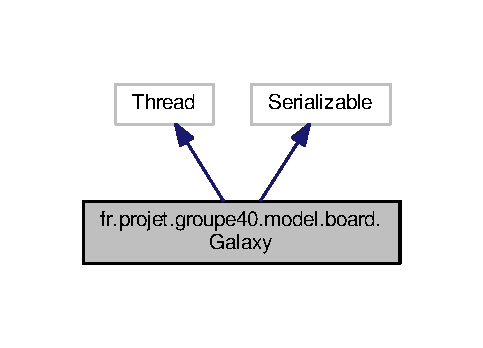
\includegraphics[width=232pt]{classfr_1_1projet_1_1groupe40_1_1model_1_1board_1_1_galaxy__inherit__graph}
\end{center}
\end{figure}


Collaboration diagram for fr.\+projet.\+groupe40.\+model.\+board.\+Galaxy\+:\nopagebreak
\begin{figure}[H]
\begin{center}
\leavevmode
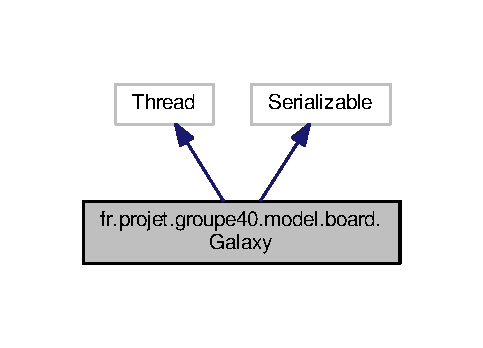
\includegraphics[width=232pt]{classfr_1_1projet_1_1groupe40_1_1model_1_1board_1_1_galaxy__coll__graph}
\end{center}
\end{figure}
\subsection*{Public Member Functions}
\begin{DoxyCompactItemize}
\item 
\hyperlink{classfr_1_1projet_1_1groupe40_1_1model_1_1board_1_1_galaxy_a9fc182ce74a25f23495edadbac56e787}{Galaxy} ()
\begin{DoxyCompactList}\small\item\em Generate a game board with every parameters randomized. \end{DoxyCompactList}\item 
\hyperlink{classfr_1_1projet_1_1groupe40_1_1model_1_1board_1_1_galaxy_adf41b1524b98b0fc609d3f8950aa2c62}{Galaxy} (\hyperlink{classfr_1_1projet_1_1groupe40_1_1model_1_1board_1_1_galaxy}{Galaxy} g)
\begin{DoxyCompactList}\small\item\em Generate a game board from another. \end{DoxyCompactList}\item 
\hyperlink{classfr_1_1projet_1_1groupe40_1_1model_1_1board_1_1_galaxy_af97d7f23693a211e91502348f0f06add}{Galaxy} (List$<$ \hyperlink{classfr_1_1projet_1_1groupe40_1_1model_1_1board_1_1_planet}{Planet} $>$ planets, List$<$ \hyperlink{classfr_1_1projet_1_1groupe40_1_1model_1_1ships_1_1_squad}{Squad} $>$ squads)
\begin{DoxyCompactList}\small\item\em Generate a game board from an array of squads and planets. \end{DoxyCompactList}\item 
void \hyperlink{classfr_1_1projet_1_1groupe40_1_1model_1_1board_1_1_galaxy_ae111f4acddd20f276118c6190fe377e7}{run} ()
\begin{DoxyCompactList}\small\item\em Thread updating the garrison value for each planets / 1 second. \end{DoxyCompactList}\item 
void \hyperlink{classfr_1_1projet_1_1groupe40_1_1model_1_1board_1_1_galaxy_a9758b40b129bd15cea53011c4c632034}{stop\+Thread} ()
\begin{DoxyCompactList}\small\item\em Stop the thread updating the garrison when called. \end{DoxyCompactList}\item 
void \hyperlink{classfr_1_1projet_1_1groupe40_1_1model_1_1board_1_1_galaxy_a4d87d109c4c08d5b6047b7fe6c35a2e6}{render} (Graphics\+Context gc)
\item 
void \hyperlink{classfr_1_1projet_1_1groupe40_1_1model_1_1board_1_1_galaxy_a26524a88f939563e1a433a5caebd5f31}{update} ()
\begin{DoxyCompactList}\small\item\em Main update function, manage AI, squads and has\+Lost. \end{DoxyCompactList}\item 
void \hyperlink{classfr_1_1projet_1_1groupe40_1_1model_1_1board_1_1_galaxy_a94ac22bfc0d4692c0cb68290dafefb62}{update\+Squad} ()
\begin{DoxyCompactList}\small\item\em Update every squads position on board. \end{DoxyCompactList}\item 
void \hyperlink{classfr_1_1projet_1_1groupe40_1_1model_1_1board_1_1_galaxy_a3845928fc6782971d4e687bf0371cae6}{update\+AI} ()
\begin{DoxyCompactList}\small\item\em Manage the AI to send fleets. \end{DoxyCompactList}\item 
boolean \hyperlink{classfr_1_1projet_1_1groupe40_1_1model_1_1board_1_1_galaxy_a95097e70a3cdd31b4ac52821851183e3}{user\+Has\+Lost} (\hyperlink{classfr_1_1projet_1_1groupe40_1_1client_1_1_user}{User} u)
\begin{DoxyCompactList}\small\item\em Check if an user has lost. \end{DoxyCompactList}\item 
void \hyperlink{classfr_1_1projet_1_1groupe40_1_1model_1_1board_1_1_galaxy_aa1dca5048cce816bb712466832a76264}{client\+Scroll\+Handler} (int action)
\begin{DoxyCompactList}\small\item\em handle the scrolls event to change the percent of a fleet to send \end{DoxyCompactList}\item 
void \hyperlink{classfr_1_1projet_1_1groupe40_1_1model_1_1board_1_1_galaxy_a2c14094cc08d7efa6fc63624bd479e5e}{collision\+Handler} (\hyperlink{classfr_1_1projet_1_1groupe40_1_1model_1_1ships_1_1_squad}{Squad} s, \hyperlink{classfr_1_1projet_1_1groupe40_1_1model_1_1board_1_1_planet}{Planet} p)
\begin{DoxyCompactList}\small\item\em Manage the collisions between squads \& intermediate planets. \end{DoxyCompactList}\item 
boolean \hyperlink{classfr_1_1projet_1_1groupe40_1_1model_1_1board_1_1_galaxy_af0fc1142e337409617e0508c57ecce55}{is\+Collision} (\hyperlink{classfr_1_1projet_1_1groupe40_1_1model_1_1ships_1_1_squad}{Squad} s)
\begin{DoxyCompactList}\small\item\em check if there s a collision between a squad and every planet on board \end{DoxyCompactList}\item 
void \hyperlink{classfr_1_1projet_1_1groupe40_1_1model_1_1board_1_1_galaxy_aff898566fd28de2e9af973395d063790}{generate\+Planets} ()
\begin{DoxyCompactList}\small\item\em Generate the planets for the galaxy initialization. \end{DoxyCompactList}\item 
void \hyperlink{classfr_1_1projet_1_1groupe40_1_1model_1_1board_1_1_galaxy_a587e7baee3f8b1d8806346c100168bac}{generate\+Random\+Squads} ()
\item 
void \hyperlink{classfr_1_1projet_1_1groupe40_1_1model_1_1board_1_1_galaxy_a6c7e549103e7eba271b1beb9fdb36720}{render\+Background} (Graphics\+Context gc)
\begin{DoxyCompactList}\small\item\em Render the background image. \end{DoxyCompactList}\item 
void \hyperlink{classfr_1_1projet_1_1groupe40_1_1model_1_1board_1_1_galaxy_ad5bd6b40a74a4cacb1c6ca2ac92f9d75}{render\+Planets} (Graphics\+Context gc)
\begin{DoxyCompactList}\small\item\em Render each planets image. \end{DoxyCompactList}\item 
void \hyperlink{classfr_1_1projet_1_1groupe40_1_1model_1_1board_1_1_galaxy_a2af7b41f184f8052f51955ac23ee6b7c}{render\+Squads} (Graphics\+Context gc)
\begin{DoxyCompactList}\small\item\em Render every squads on board. \end{DoxyCompactList}\item 
void \hyperlink{classfr_1_1projet_1_1groupe40_1_1model_1_1board_1_1_galaxy_a9d6bfd8ae13a74eb18e9b75fc12ffafd}{render\+Garrison} (Graphics\+Context gc)
\begin{DoxyCompactList}\small\item\em Render the garrison amount of each planets on board. \end{DoxyCompactList}\item 
void \hyperlink{classfr_1_1projet_1_1groupe40_1_1model_1_1board_1_1_galaxy_a1785a032d6611d092033ff81e0b688d2}{render\+Percentage\+Selected} (Graphics\+Context gc)
\begin{DoxyCompactList}\small\item\em Render the percentage of troups to send selected by the player. \end{DoxyCompactList}\item 
void \hyperlink{classfr_1_1projet_1_1groupe40_1_1model_1_1board_1_1_galaxy_a3997b2f9daacabfa4ceb38b129f56f3e}{render\+Explosion} (Graphics\+Context gc)
\begin{DoxyCompactList}\small\item\em render a explosion when a ship reach his destination \end{DoxyCompactList}\item 
void \hyperlink{classfr_1_1projet_1_1groupe40_1_1model_1_1board_1_1_galaxy_a6f31adbe336406cbc701d769ac03d0b8}{init\+Font} (Graphics\+Context gc)
\begin{DoxyCompactList}\small\item\em Init the default font style of the graphics context. \end{DoxyCompactList}\item 
Array\+List$<$ \hyperlink{classfr_1_1projet_1_1groupe40_1_1model_1_1ships_1_1_squad}{Squad} $>$ \hyperlink{classfr_1_1projet_1_1groupe40_1_1model_1_1board_1_1_galaxy_a22d431ce871b313fbeb72004e2fbcac8}{get\+Squads} ()
\begin{DoxyCompactList}\small\item\em Set the list containing every squads by another one. \end{DoxyCompactList}\item 
void \hyperlink{classfr_1_1projet_1_1groupe40_1_1model_1_1board_1_1_galaxy_afdfdd3a32fa34be534eb436d4fd70788}{set\+Squads} (Array\+List$<$ \hyperlink{classfr_1_1projet_1_1groupe40_1_1model_1_1ships_1_1_squad}{Squad} $>$ squads)
\begin{DoxyCompactList}\small\item\em Return the list containing every squads on board. \end{DoxyCompactList}\item 
void \hyperlink{classfr_1_1projet_1_1groupe40_1_1model_1_1board_1_1_galaxy_a22ae6c3d0f709f614e232d3122c7b9b4}{set\+Planets} (Array\+List$<$ \hyperlink{classfr_1_1projet_1_1groupe40_1_1model_1_1board_1_1_planet}{Planet} $>$ planets)
\begin{DoxyCompactList}\small\item\em Set the list containing every planet by another one. \end{DoxyCompactList}\item 
Array\+List$<$ \hyperlink{classfr_1_1projet_1_1groupe40_1_1model_1_1board_1_1_planet}{Planet} $>$ \hyperlink{classfr_1_1projet_1_1groupe40_1_1model_1_1board_1_1_galaxy_ab6db29c36ed37b5c2e6c08ee62cd9040}{get\+Planets} ()
\begin{DoxyCompactList}\small\item\em Return the list containing every planets on board. \end{DoxyCompactList}\item 
Image \hyperlink{classfr_1_1projet_1_1groupe40_1_1model_1_1board_1_1_galaxy_afcccc9ebe565d321f0c6bf1cd49e4676}{get\+Background} ()
\begin{DoxyCompactList}\small\item\em Return the background image. \end{DoxyCompactList}\item 
void \hyperlink{classfr_1_1projet_1_1groupe40_1_1model_1_1board_1_1_galaxy_adcb4e80619863342931153460e92f4a7}{set\+Background} (Image background)
\begin{DoxyCompactList}\small\item\em Set the background image. \end{DoxyCompactList}\end{DoxyCompactItemize}


\subsection{Constructor \& Destructor Documentation}
\mbox{\Hypertarget{classfr_1_1projet_1_1groupe40_1_1model_1_1board_1_1_galaxy_a9fc182ce74a25f23495edadbac56e787}\label{classfr_1_1projet_1_1groupe40_1_1model_1_1board_1_1_galaxy_a9fc182ce74a25f23495edadbac56e787}} 
\index{fr\+::projet\+::groupe40\+::model\+::board\+::\+Galaxy@{fr\+::projet\+::groupe40\+::model\+::board\+::\+Galaxy}!Galaxy@{Galaxy}}
\index{Galaxy@{Galaxy}!fr\+::projet\+::groupe40\+::model\+::board\+::\+Galaxy@{fr\+::projet\+::groupe40\+::model\+::board\+::\+Galaxy}}
\subsubsection{\texorpdfstring{Galaxy()}{Galaxy()}\hspace{0.1cm}{\footnotesize\ttfamily [1/3]}}
{\footnotesize\ttfamily fr.\+projet.\+groupe40.\+model.\+board.\+Galaxy.\+Galaxy (\begin{DoxyParamCaption}{ }\end{DoxyParamCaption})}



Generate a game board with every parameters randomized. 

\mbox{\Hypertarget{classfr_1_1projet_1_1groupe40_1_1model_1_1board_1_1_galaxy_adf41b1524b98b0fc609d3f8950aa2c62}\label{classfr_1_1projet_1_1groupe40_1_1model_1_1board_1_1_galaxy_adf41b1524b98b0fc609d3f8950aa2c62}} 
\index{fr\+::projet\+::groupe40\+::model\+::board\+::\+Galaxy@{fr\+::projet\+::groupe40\+::model\+::board\+::\+Galaxy}!Galaxy@{Galaxy}}
\index{Galaxy@{Galaxy}!fr\+::projet\+::groupe40\+::model\+::board\+::\+Galaxy@{fr\+::projet\+::groupe40\+::model\+::board\+::\+Galaxy}}
\subsubsection{\texorpdfstring{Galaxy()}{Galaxy()}\hspace{0.1cm}{\footnotesize\ttfamily [2/3]}}
{\footnotesize\ttfamily fr.\+projet.\+groupe40.\+model.\+board.\+Galaxy.\+Galaxy (\begin{DoxyParamCaption}\item[{\hyperlink{classfr_1_1projet_1_1groupe40_1_1model_1_1board_1_1_galaxy}{Galaxy}}]{g }\end{DoxyParamCaption})}



Generate a game board from another. 


\begin{DoxyParams}{Parameters}
{\em g} & The game board to copy from \\
\hline
\end{DoxyParams}
\mbox{\Hypertarget{classfr_1_1projet_1_1groupe40_1_1model_1_1board_1_1_galaxy_af97d7f23693a211e91502348f0f06add}\label{classfr_1_1projet_1_1groupe40_1_1model_1_1board_1_1_galaxy_af97d7f23693a211e91502348f0f06add}} 
\index{fr\+::projet\+::groupe40\+::model\+::board\+::\+Galaxy@{fr\+::projet\+::groupe40\+::model\+::board\+::\+Galaxy}!Galaxy@{Galaxy}}
\index{Galaxy@{Galaxy}!fr\+::projet\+::groupe40\+::model\+::board\+::\+Galaxy@{fr\+::projet\+::groupe40\+::model\+::board\+::\+Galaxy}}
\subsubsection{\texorpdfstring{Galaxy()}{Galaxy()}\hspace{0.1cm}{\footnotesize\ttfamily [3/3]}}
{\footnotesize\ttfamily fr.\+projet.\+groupe40.\+model.\+board.\+Galaxy.\+Galaxy (\begin{DoxyParamCaption}\item[{List$<$ \hyperlink{classfr_1_1projet_1_1groupe40_1_1model_1_1board_1_1_planet}{Planet} $>$}]{planets,  }\item[{List$<$ \hyperlink{classfr_1_1projet_1_1groupe40_1_1model_1_1ships_1_1_squad}{Squad} $>$}]{squads }\end{DoxyParamCaption})}



Generate a game board from an array of squads and planets. 


\begin{DoxyParams}{Parameters}
{\em planets} & Planets that we want to have \\
\hline
{\em squads} & Squads already present \\
\hline
\end{DoxyParams}


\subsection{Member Function Documentation}
\mbox{\Hypertarget{classfr_1_1projet_1_1groupe40_1_1model_1_1board_1_1_galaxy_aa1dca5048cce816bb712466832a76264}\label{classfr_1_1projet_1_1groupe40_1_1model_1_1board_1_1_galaxy_aa1dca5048cce816bb712466832a76264}} 
\index{fr\+::projet\+::groupe40\+::model\+::board\+::\+Galaxy@{fr\+::projet\+::groupe40\+::model\+::board\+::\+Galaxy}!client\+Scroll\+Handler@{client\+Scroll\+Handler}}
\index{client\+Scroll\+Handler@{client\+Scroll\+Handler}!fr\+::projet\+::groupe40\+::model\+::board\+::\+Galaxy@{fr\+::projet\+::groupe40\+::model\+::board\+::\+Galaxy}}
\subsubsection{\texorpdfstring{client\+Scroll\+Handler()}{clientScrollHandler()}}
{\footnotesize\ttfamily void fr.\+projet.\+groupe40.\+model.\+board.\+Galaxy.\+client\+Scroll\+Handler (\begin{DoxyParamCaption}\item[{int}]{action }\end{DoxyParamCaption})}



handle the scrolls event to change the percent of a fleet to send 


\begin{DoxyParams}{Parameters}
{\em action} & The scroll action (up or down case) \\
\hline
\end{DoxyParams}
\mbox{\Hypertarget{classfr_1_1projet_1_1groupe40_1_1model_1_1board_1_1_galaxy_a2c14094cc08d7efa6fc63624bd479e5e}\label{classfr_1_1projet_1_1groupe40_1_1model_1_1board_1_1_galaxy_a2c14094cc08d7efa6fc63624bd479e5e}} 
\index{fr\+::projet\+::groupe40\+::model\+::board\+::\+Galaxy@{fr\+::projet\+::groupe40\+::model\+::board\+::\+Galaxy}!collision\+Handler@{collision\+Handler}}
\index{collision\+Handler@{collision\+Handler}!fr\+::projet\+::groupe40\+::model\+::board\+::\+Galaxy@{fr\+::projet\+::groupe40\+::model\+::board\+::\+Galaxy}}
\subsubsection{\texorpdfstring{collision\+Handler()}{collisionHandler()}}
{\footnotesize\ttfamily void fr.\+projet.\+groupe40.\+model.\+board.\+Galaxy.\+collision\+Handler (\begin{DoxyParamCaption}\item[{\hyperlink{classfr_1_1projet_1_1groupe40_1_1model_1_1ships_1_1_squad}{Squad}}]{s,  }\item[{\hyperlink{classfr_1_1projet_1_1groupe40_1_1model_1_1board_1_1_planet}{Planet}}]{p }\end{DoxyParamCaption})}



Manage the collisions between squads \& intermediate planets. 


\begin{DoxyParams}{Parameters}
{\em s} & The squad to manage \\
\hline
{\em p} & The planet to test collision with \\
\hline
\end{DoxyParams}
\mbox{\Hypertarget{classfr_1_1projet_1_1groupe40_1_1model_1_1board_1_1_galaxy_aff898566fd28de2e9af973395d063790}\label{classfr_1_1projet_1_1groupe40_1_1model_1_1board_1_1_galaxy_aff898566fd28de2e9af973395d063790}} 
\index{fr\+::projet\+::groupe40\+::model\+::board\+::\+Galaxy@{fr\+::projet\+::groupe40\+::model\+::board\+::\+Galaxy}!generate\+Planets@{generate\+Planets}}
\index{generate\+Planets@{generate\+Planets}!fr\+::projet\+::groupe40\+::model\+::board\+::\+Galaxy@{fr\+::projet\+::groupe40\+::model\+::board\+::\+Galaxy}}
\subsubsection{\texorpdfstring{generate\+Planets()}{generatePlanets()}}
{\footnotesize\ttfamily void fr.\+projet.\+groupe40.\+model.\+board.\+Galaxy.\+generate\+Planets (\begin{DoxyParamCaption}{ }\end{DoxyParamCaption})}



Generate the planets for the galaxy initialization. 

\mbox{\Hypertarget{classfr_1_1projet_1_1groupe40_1_1model_1_1board_1_1_galaxy_a587e7baee3f8b1d8806346c100168bac}\label{classfr_1_1projet_1_1groupe40_1_1model_1_1board_1_1_galaxy_a587e7baee3f8b1d8806346c100168bac}} 
\index{fr\+::projet\+::groupe40\+::model\+::board\+::\+Galaxy@{fr\+::projet\+::groupe40\+::model\+::board\+::\+Galaxy}!generate\+Random\+Squads@{generate\+Random\+Squads}}
\index{generate\+Random\+Squads@{generate\+Random\+Squads}!fr\+::projet\+::groupe40\+::model\+::board\+::\+Galaxy@{fr\+::projet\+::groupe40\+::model\+::board\+::\+Galaxy}}
\subsubsection{\texorpdfstring{generate\+Random\+Squads()}{generateRandomSquads()}}
{\footnotesize\ttfamily void fr.\+projet.\+groupe40.\+model.\+board.\+Galaxy.\+generate\+Random\+Squads (\begin{DoxyParamCaption}{ }\end{DoxyParamCaption})}

\mbox{\Hypertarget{classfr_1_1projet_1_1groupe40_1_1model_1_1board_1_1_galaxy_afcccc9ebe565d321f0c6bf1cd49e4676}\label{classfr_1_1projet_1_1groupe40_1_1model_1_1board_1_1_galaxy_afcccc9ebe565d321f0c6bf1cd49e4676}} 
\index{fr\+::projet\+::groupe40\+::model\+::board\+::\+Galaxy@{fr\+::projet\+::groupe40\+::model\+::board\+::\+Galaxy}!get\+Background@{get\+Background}}
\index{get\+Background@{get\+Background}!fr\+::projet\+::groupe40\+::model\+::board\+::\+Galaxy@{fr\+::projet\+::groupe40\+::model\+::board\+::\+Galaxy}}
\subsubsection{\texorpdfstring{get\+Background()}{getBackground()}}
{\footnotesize\ttfamily Image fr.\+projet.\+groupe40.\+model.\+board.\+Galaxy.\+get\+Background (\begin{DoxyParamCaption}{ }\end{DoxyParamCaption})}



Return the background image. 

\begin{DoxyReturn}{Returns}
Image 
\end{DoxyReturn}
\mbox{\Hypertarget{classfr_1_1projet_1_1groupe40_1_1model_1_1board_1_1_galaxy_ab6db29c36ed37b5c2e6c08ee62cd9040}\label{classfr_1_1projet_1_1groupe40_1_1model_1_1board_1_1_galaxy_ab6db29c36ed37b5c2e6c08ee62cd9040}} 
\index{fr\+::projet\+::groupe40\+::model\+::board\+::\+Galaxy@{fr\+::projet\+::groupe40\+::model\+::board\+::\+Galaxy}!get\+Planets@{get\+Planets}}
\index{get\+Planets@{get\+Planets}!fr\+::projet\+::groupe40\+::model\+::board\+::\+Galaxy@{fr\+::projet\+::groupe40\+::model\+::board\+::\+Galaxy}}
\subsubsection{\texorpdfstring{get\+Planets()}{getPlanets()}}
{\footnotesize\ttfamily Array\+List$<$\hyperlink{classfr_1_1projet_1_1groupe40_1_1model_1_1board_1_1_planet}{Planet}$>$ fr.\+projet.\+groupe40.\+model.\+board.\+Galaxy.\+get\+Planets (\begin{DoxyParamCaption}{ }\end{DoxyParamCaption})}



Return the list containing every planets on board. 

\begin{DoxyReturn}{Returns}

\end{DoxyReturn}
\mbox{\Hypertarget{classfr_1_1projet_1_1groupe40_1_1model_1_1board_1_1_galaxy_a22d431ce871b313fbeb72004e2fbcac8}\label{classfr_1_1projet_1_1groupe40_1_1model_1_1board_1_1_galaxy_a22d431ce871b313fbeb72004e2fbcac8}} 
\index{fr\+::projet\+::groupe40\+::model\+::board\+::\+Galaxy@{fr\+::projet\+::groupe40\+::model\+::board\+::\+Galaxy}!get\+Squads@{get\+Squads}}
\index{get\+Squads@{get\+Squads}!fr\+::projet\+::groupe40\+::model\+::board\+::\+Galaxy@{fr\+::projet\+::groupe40\+::model\+::board\+::\+Galaxy}}
\subsubsection{\texorpdfstring{get\+Squads()}{getSquads()}}
{\footnotesize\ttfamily Array\+List$<$\hyperlink{classfr_1_1projet_1_1groupe40_1_1model_1_1ships_1_1_squad}{Squad}$>$ fr.\+projet.\+groupe40.\+model.\+board.\+Galaxy.\+get\+Squads (\begin{DoxyParamCaption}{ }\end{DoxyParamCaption})}



Set the list containing every squads by another one. 


\begin{DoxyParams}{Parameters}
{\em planets} & \\
\hline
\end{DoxyParams}
\mbox{\Hypertarget{classfr_1_1projet_1_1groupe40_1_1model_1_1board_1_1_galaxy_a6f31adbe336406cbc701d769ac03d0b8}\label{classfr_1_1projet_1_1groupe40_1_1model_1_1board_1_1_galaxy_a6f31adbe336406cbc701d769ac03d0b8}} 
\index{fr\+::projet\+::groupe40\+::model\+::board\+::\+Galaxy@{fr\+::projet\+::groupe40\+::model\+::board\+::\+Galaxy}!init\+Font@{init\+Font}}
\index{init\+Font@{init\+Font}!fr\+::projet\+::groupe40\+::model\+::board\+::\+Galaxy@{fr\+::projet\+::groupe40\+::model\+::board\+::\+Galaxy}}
\subsubsection{\texorpdfstring{init\+Font()}{initFont()}}
{\footnotesize\ttfamily void fr.\+projet.\+groupe40.\+model.\+board.\+Galaxy.\+init\+Font (\begin{DoxyParamCaption}\item[{Graphics\+Context}]{gc }\end{DoxyParamCaption})}



Init the default font style of the graphics context. 


\begin{DoxyParams}{Parameters}
{\em gc} & \\
\hline
\end{DoxyParams}
\mbox{\Hypertarget{classfr_1_1projet_1_1groupe40_1_1model_1_1board_1_1_galaxy_af0fc1142e337409617e0508c57ecce55}\label{classfr_1_1projet_1_1groupe40_1_1model_1_1board_1_1_galaxy_af0fc1142e337409617e0508c57ecce55}} 
\index{fr\+::projet\+::groupe40\+::model\+::board\+::\+Galaxy@{fr\+::projet\+::groupe40\+::model\+::board\+::\+Galaxy}!is\+Collision@{is\+Collision}}
\index{is\+Collision@{is\+Collision}!fr\+::projet\+::groupe40\+::model\+::board\+::\+Galaxy@{fr\+::projet\+::groupe40\+::model\+::board\+::\+Galaxy}}
\subsubsection{\texorpdfstring{is\+Collision()}{isCollision()}}
{\footnotesize\ttfamily boolean fr.\+projet.\+groupe40.\+model.\+board.\+Galaxy.\+is\+Collision (\begin{DoxyParamCaption}\item[{\hyperlink{classfr_1_1projet_1_1groupe40_1_1model_1_1ships_1_1_squad}{Squad}}]{s }\end{DoxyParamCaption})}



check if there s a collision between a squad and every planet on board 


\begin{DoxyParams}{Parameters}
{\em s} & the squad to check \\
\hline
\end{DoxyParams}
\begin{DoxyReturn}{Returns}
true if there s a collision, else false 
\end{DoxyReturn}
\mbox{\Hypertarget{classfr_1_1projet_1_1groupe40_1_1model_1_1board_1_1_galaxy_a4d87d109c4c08d5b6047b7fe6c35a2e6}\label{classfr_1_1projet_1_1groupe40_1_1model_1_1board_1_1_galaxy_a4d87d109c4c08d5b6047b7fe6c35a2e6}} 
\index{fr\+::projet\+::groupe40\+::model\+::board\+::\+Galaxy@{fr\+::projet\+::groupe40\+::model\+::board\+::\+Galaxy}!render@{render}}
\index{render@{render}!fr\+::projet\+::groupe40\+::model\+::board\+::\+Galaxy@{fr\+::projet\+::groupe40\+::model\+::board\+::\+Galaxy}}
\subsubsection{\texorpdfstring{render()}{render()}}
{\footnotesize\ttfamily void fr.\+projet.\+groupe40.\+model.\+board.\+Galaxy.\+render (\begin{DoxyParamCaption}\item[{Graphics\+Context}]{gc }\end{DoxyParamCaption})}

Main rendering function 
\begin{DoxyParams}{Parameters}
{\em gc} & \\
\hline
\end{DoxyParams}
\mbox{\Hypertarget{classfr_1_1projet_1_1groupe40_1_1model_1_1board_1_1_galaxy_a6c7e549103e7eba271b1beb9fdb36720}\label{classfr_1_1projet_1_1groupe40_1_1model_1_1board_1_1_galaxy_a6c7e549103e7eba271b1beb9fdb36720}} 
\index{fr\+::projet\+::groupe40\+::model\+::board\+::\+Galaxy@{fr\+::projet\+::groupe40\+::model\+::board\+::\+Galaxy}!render\+Background@{render\+Background}}
\index{render\+Background@{render\+Background}!fr\+::projet\+::groupe40\+::model\+::board\+::\+Galaxy@{fr\+::projet\+::groupe40\+::model\+::board\+::\+Galaxy}}
\subsubsection{\texorpdfstring{render\+Background()}{renderBackground()}}
{\footnotesize\ttfamily void fr.\+projet.\+groupe40.\+model.\+board.\+Galaxy.\+render\+Background (\begin{DoxyParamCaption}\item[{Graphics\+Context}]{gc }\end{DoxyParamCaption})}



Render the background image. 


\begin{DoxyParams}{Parameters}
{\em gc} & \\
\hline
\end{DoxyParams}
\mbox{\Hypertarget{classfr_1_1projet_1_1groupe40_1_1model_1_1board_1_1_galaxy_a3997b2f9daacabfa4ceb38b129f56f3e}\label{classfr_1_1projet_1_1groupe40_1_1model_1_1board_1_1_galaxy_a3997b2f9daacabfa4ceb38b129f56f3e}} 
\index{fr\+::projet\+::groupe40\+::model\+::board\+::\+Galaxy@{fr\+::projet\+::groupe40\+::model\+::board\+::\+Galaxy}!render\+Explosion@{render\+Explosion}}
\index{render\+Explosion@{render\+Explosion}!fr\+::projet\+::groupe40\+::model\+::board\+::\+Galaxy@{fr\+::projet\+::groupe40\+::model\+::board\+::\+Galaxy}}
\subsubsection{\texorpdfstring{render\+Explosion()}{renderExplosion()}}
{\footnotesize\ttfamily void fr.\+projet.\+groupe40.\+model.\+board.\+Galaxy.\+render\+Explosion (\begin{DoxyParamCaption}\item[{Graphics\+Context}]{gc }\end{DoxyParamCaption})}



render a explosion when a ship reach his destination 


\begin{DoxyParams}{Parameters}
{\em gc} & \\
\hline
\end{DoxyParams}
\mbox{\Hypertarget{classfr_1_1projet_1_1groupe40_1_1model_1_1board_1_1_galaxy_a9d6bfd8ae13a74eb18e9b75fc12ffafd}\label{classfr_1_1projet_1_1groupe40_1_1model_1_1board_1_1_galaxy_a9d6bfd8ae13a74eb18e9b75fc12ffafd}} 
\index{fr\+::projet\+::groupe40\+::model\+::board\+::\+Galaxy@{fr\+::projet\+::groupe40\+::model\+::board\+::\+Galaxy}!render\+Garrison@{render\+Garrison}}
\index{render\+Garrison@{render\+Garrison}!fr\+::projet\+::groupe40\+::model\+::board\+::\+Galaxy@{fr\+::projet\+::groupe40\+::model\+::board\+::\+Galaxy}}
\subsubsection{\texorpdfstring{render\+Garrison()}{renderGarrison()}}
{\footnotesize\ttfamily void fr.\+projet.\+groupe40.\+model.\+board.\+Galaxy.\+render\+Garrison (\begin{DoxyParamCaption}\item[{Graphics\+Context}]{gc }\end{DoxyParamCaption})}



Render the garrison amount of each planets on board. 


\begin{DoxyParams}{Parameters}
{\em gc} & \\
\hline
\end{DoxyParams}
\mbox{\Hypertarget{classfr_1_1projet_1_1groupe40_1_1model_1_1board_1_1_galaxy_a1785a032d6611d092033ff81e0b688d2}\label{classfr_1_1projet_1_1groupe40_1_1model_1_1board_1_1_galaxy_a1785a032d6611d092033ff81e0b688d2}} 
\index{fr\+::projet\+::groupe40\+::model\+::board\+::\+Galaxy@{fr\+::projet\+::groupe40\+::model\+::board\+::\+Galaxy}!render\+Percentage\+Selected@{render\+Percentage\+Selected}}
\index{render\+Percentage\+Selected@{render\+Percentage\+Selected}!fr\+::projet\+::groupe40\+::model\+::board\+::\+Galaxy@{fr\+::projet\+::groupe40\+::model\+::board\+::\+Galaxy}}
\subsubsection{\texorpdfstring{render\+Percentage\+Selected()}{renderPercentageSelected()}}
{\footnotesize\ttfamily void fr.\+projet.\+groupe40.\+model.\+board.\+Galaxy.\+render\+Percentage\+Selected (\begin{DoxyParamCaption}\item[{Graphics\+Context}]{gc }\end{DoxyParamCaption})}



Render the percentage of troups to send selected by the player. 


\begin{DoxyParams}{Parameters}
{\em gc} & \\
\hline
\end{DoxyParams}
\mbox{\Hypertarget{classfr_1_1projet_1_1groupe40_1_1model_1_1board_1_1_galaxy_ad5bd6b40a74a4cacb1c6ca2ac92f9d75}\label{classfr_1_1projet_1_1groupe40_1_1model_1_1board_1_1_galaxy_ad5bd6b40a74a4cacb1c6ca2ac92f9d75}} 
\index{fr\+::projet\+::groupe40\+::model\+::board\+::\+Galaxy@{fr\+::projet\+::groupe40\+::model\+::board\+::\+Galaxy}!render\+Planets@{render\+Planets}}
\index{render\+Planets@{render\+Planets}!fr\+::projet\+::groupe40\+::model\+::board\+::\+Galaxy@{fr\+::projet\+::groupe40\+::model\+::board\+::\+Galaxy}}
\subsubsection{\texorpdfstring{render\+Planets()}{renderPlanets()}}
{\footnotesize\ttfamily void fr.\+projet.\+groupe40.\+model.\+board.\+Galaxy.\+render\+Planets (\begin{DoxyParamCaption}\item[{Graphics\+Context}]{gc }\end{DoxyParamCaption})}



Render each planets image. 


\begin{DoxyParams}{Parameters}
{\em gc} & \\
\hline
\end{DoxyParams}
\mbox{\Hypertarget{classfr_1_1projet_1_1groupe40_1_1model_1_1board_1_1_galaxy_a2af7b41f184f8052f51955ac23ee6b7c}\label{classfr_1_1projet_1_1groupe40_1_1model_1_1board_1_1_galaxy_a2af7b41f184f8052f51955ac23ee6b7c}} 
\index{fr\+::projet\+::groupe40\+::model\+::board\+::\+Galaxy@{fr\+::projet\+::groupe40\+::model\+::board\+::\+Galaxy}!render\+Squads@{render\+Squads}}
\index{render\+Squads@{render\+Squads}!fr\+::projet\+::groupe40\+::model\+::board\+::\+Galaxy@{fr\+::projet\+::groupe40\+::model\+::board\+::\+Galaxy}}
\subsubsection{\texorpdfstring{render\+Squads()}{renderSquads()}}
{\footnotesize\ttfamily void fr.\+projet.\+groupe40.\+model.\+board.\+Galaxy.\+render\+Squads (\begin{DoxyParamCaption}\item[{Graphics\+Context}]{gc }\end{DoxyParamCaption})}



Render every squads on board. 


\begin{DoxyParams}{Parameters}
{\em gc} & \\
\hline
\end{DoxyParams}
\mbox{\Hypertarget{classfr_1_1projet_1_1groupe40_1_1model_1_1board_1_1_galaxy_ae111f4acddd20f276118c6190fe377e7}\label{classfr_1_1projet_1_1groupe40_1_1model_1_1board_1_1_galaxy_ae111f4acddd20f276118c6190fe377e7}} 
\index{fr\+::projet\+::groupe40\+::model\+::board\+::\+Galaxy@{fr\+::projet\+::groupe40\+::model\+::board\+::\+Galaxy}!run@{run}}
\index{run@{run}!fr\+::projet\+::groupe40\+::model\+::board\+::\+Galaxy@{fr\+::projet\+::groupe40\+::model\+::board\+::\+Galaxy}}
\subsubsection{\texorpdfstring{run()}{run()}}
{\footnotesize\ttfamily void fr.\+projet.\+groupe40.\+model.\+board.\+Galaxy.\+run (\begin{DoxyParamCaption}{ }\end{DoxyParamCaption})}



Thread updating the garrison value for each planets / 1 second. 

\mbox{\Hypertarget{classfr_1_1projet_1_1groupe40_1_1model_1_1board_1_1_galaxy_adcb4e80619863342931153460e92f4a7}\label{classfr_1_1projet_1_1groupe40_1_1model_1_1board_1_1_galaxy_adcb4e80619863342931153460e92f4a7}} 
\index{fr\+::projet\+::groupe40\+::model\+::board\+::\+Galaxy@{fr\+::projet\+::groupe40\+::model\+::board\+::\+Galaxy}!set\+Background@{set\+Background}}
\index{set\+Background@{set\+Background}!fr\+::projet\+::groupe40\+::model\+::board\+::\+Galaxy@{fr\+::projet\+::groupe40\+::model\+::board\+::\+Galaxy}}
\subsubsection{\texorpdfstring{set\+Background()}{setBackground()}}
{\footnotesize\ttfamily void fr.\+projet.\+groupe40.\+model.\+board.\+Galaxy.\+set\+Background (\begin{DoxyParamCaption}\item[{Image}]{background }\end{DoxyParamCaption})}



Set the background image. 


\begin{DoxyParams}{Parameters}
{\em background} & \\
\hline
\end{DoxyParams}
\mbox{\Hypertarget{classfr_1_1projet_1_1groupe40_1_1model_1_1board_1_1_galaxy_a22ae6c3d0f709f614e232d3122c7b9b4}\label{classfr_1_1projet_1_1groupe40_1_1model_1_1board_1_1_galaxy_a22ae6c3d0f709f614e232d3122c7b9b4}} 
\index{fr\+::projet\+::groupe40\+::model\+::board\+::\+Galaxy@{fr\+::projet\+::groupe40\+::model\+::board\+::\+Galaxy}!set\+Planets@{set\+Planets}}
\index{set\+Planets@{set\+Planets}!fr\+::projet\+::groupe40\+::model\+::board\+::\+Galaxy@{fr\+::projet\+::groupe40\+::model\+::board\+::\+Galaxy}}
\subsubsection{\texorpdfstring{set\+Planets()}{setPlanets()}}
{\footnotesize\ttfamily void fr.\+projet.\+groupe40.\+model.\+board.\+Galaxy.\+set\+Planets (\begin{DoxyParamCaption}\item[{Array\+List$<$ \hyperlink{classfr_1_1projet_1_1groupe40_1_1model_1_1board_1_1_planet}{Planet} $>$}]{planets }\end{DoxyParamCaption})}



Set the list containing every planet by another one. 


\begin{DoxyParams}{Parameters}
{\em planets} & \\
\hline
\end{DoxyParams}
\mbox{\Hypertarget{classfr_1_1projet_1_1groupe40_1_1model_1_1board_1_1_galaxy_afdfdd3a32fa34be534eb436d4fd70788}\label{classfr_1_1projet_1_1groupe40_1_1model_1_1board_1_1_galaxy_afdfdd3a32fa34be534eb436d4fd70788}} 
\index{fr\+::projet\+::groupe40\+::model\+::board\+::\+Galaxy@{fr\+::projet\+::groupe40\+::model\+::board\+::\+Galaxy}!set\+Squads@{set\+Squads}}
\index{set\+Squads@{set\+Squads}!fr\+::projet\+::groupe40\+::model\+::board\+::\+Galaxy@{fr\+::projet\+::groupe40\+::model\+::board\+::\+Galaxy}}
\subsubsection{\texorpdfstring{set\+Squads()}{setSquads()}}
{\footnotesize\ttfamily void fr.\+projet.\+groupe40.\+model.\+board.\+Galaxy.\+set\+Squads (\begin{DoxyParamCaption}\item[{Array\+List$<$ \hyperlink{classfr_1_1projet_1_1groupe40_1_1model_1_1ships_1_1_squad}{Squad} $>$}]{squads }\end{DoxyParamCaption})}



Return the list containing every squads on board. 

\begin{DoxyReturn}{Returns}

\end{DoxyReturn}
\mbox{\Hypertarget{classfr_1_1projet_1_1groupe40_1_1model_1_1board_1_1_galaxy_a9758b40b129bd15cea53011c4c632034}\label{classfr_1_1projet_1_1groupe40_1_1model_1_1board_1_1_galaxy_a9758b40b129bd15cea53011c4c632034}} 
\index{fr\+::projet\+::groupe40\+::model\+::board\+::\+Galaxy@{fr\+::projet\+::groupe40\+::model\+::board\+::\+Galaxy}!stop\+Thread@{stop\+Thread}}
\index{stop\+Thread@{stop\+Thread}!fr\+::projet\+::groupe40\+::model\+::board\+::\+Galaxy@{fr\+::projet\+::groupe40\+::model\+::board\+::\+Galaxy}}
\subsubsection{\texorpdfstring{stop\+Thread()}{stopThread()}}
{\footnotesize\ttfamily void fr.\+projet.\+groupe40.\+model.\+board.\+Galaxy.\+stop\+Thread (\begin{DoxyParamCaption}{ }\end{DoxyParamCaption})}



Stop the thread updating the garrison when called. 

\mbox{\Hypertarget{classfr_1_1projet_1_1groupe40_1_1model_1_1board_1_1_galaxy_a26524a88f939563e1a433a5caebd5f31}\label{classfr_1_1projet_1_1groupe40_1_1model_1_1board_1_1_galaxy_a26524a88f939563e1a433a5caebd5f31}} 
\index{fr\+::projet\+::groupe40\+::model\+::board\+::\+Galaxy@{fr\+::projet\+::groupe40\+::model\+::board\+::\+Galaxy}!update@{update}}
\index{update@{update}!fr\+::projet\+::groupe40\+::model\+::board\+::\+Galaxy@{fr\+::projet\+::groupe40\+::model\+::board\+::\+Galaxy}}
\subsubsection{\texorpdfstring{update()}{update()}}
{\footnotesize\ttfamily void fr.\+projet.\+groupe40.\+model.\+board.\+Galaxy.\+update (\begin{DoxyParamCaption}{ }\end{DoxyParamCaption})}



Main update function, manage AI, squads and has\+Lost. 

\mbox{\Hypertarget{classfr_1_1projet_1_1groupe40_1_1model_1_1board_1_1_galaxy_a3845928fc6782971d4e687bf0371cae6}\label{classfr_1_1projet_1_1groupe40_1_1model_1_1board_1_1_galaxy_a3845928fc6782971d4e687bf0371cae6}} 
\index{fr\+::projet\+::groupe40\+::model\+::board\+::\+Galaxy@{fr\+::projet\+::groupe40\+::model\+::board\+::\+Galaxy}!update\+AI@{update\+AI}}
\index{update\+AI@{update\+AI}!fr\+::projet\+::groupe40\+::model\+::board\+::\+Galaxy@{fr\+::projet\+::groupe40\+::model\+::board\+::\+Galaxy}}
\subsubsection{\texorpdfstring{update\+A\+I()}{updateAI()}}
{\footnotesize\ttfamily void fr.\+projet.\+groupe40.\+model.\+board.\+Galaxy.\+update\+AI (\begin{DoxyParamCaption}{ }\end{DoxyParamCaption})}



Manage the AI to send fleets. 

\mbox{\Hypertarget{classfr_1_1projet_1_1groupe40_1_1model_1_1board_1_1_galaxy_a94ac22bfc0d4692c0cb68290dafefb62}\label{classfr_1_1projet_1_1groupe40_1_1model_1_1board_1_1_galaxy_a94ac22bfc0d4692c0cb68290dafefb62}} 
\index{fr\+::projet\+::groupe40\+::model\+::board\+::\+Galaxy@{fr\+::projet\+::groupe40\+::model\+::board\+::\+Galaxy}!update\+Squad@{update\+Squad}}
\index{update\+Squad@{update\+Squad}!fr\+::projet\+::groupe40\+::model\+::board\+::\+Galaxy@{fr\+::projet\+::groupe40\+::model\+::board\+::\+Galaxy}}
\subsubsection{\texorpdfstring{update\+Squad()}{updateSquad()}}
{\footnotesize\ttfamily void fr.\+projet.\+groupe40.\+model.\+board.\+Galaxy.\+update\+Squad (\begin{DoxyParamCaption}{ }\end{DoxyParamCaption})}



Update every squads position on board. 

\mbox{\Hypertarget{classfr_1_1projet_1_1groupe40_1_1model_1_1board_1_1_galaxy_a95097e70a3cdd31b4ac52821851183e3}\label{classfr_1_1projet_1_1groupe40_1_1model_1_1board_1_1_galaxy_a95097e70a3cdd31b4ac52821851183e3}} 
\index{fr\+::projet\+::groupe40\+::model\+::board\+::\+Galaxy@{fr\+::projet\+::groupe40\+::model\+::board\+::\+Galaxy}!user\+Has\+Lost@{user\+Has\+Lost}}
\index{user\+Has\+Lost@{user\+Has\+Lost}!fr\+::projet\+::groupe40\+::model\+::board\+::\+Galaxy@{fr\+::projet\+::groupe40\+::model\+::board\+::\+Galaxy}}
\subsubsection{\texorpdfstring{user\+Has\+Lost()}{userHasLost()}}
{\footnotesize\ttfamily boolean fr.\+projet.\+groupe40.\+model.\+board.\+Galaxy.\+user\+Has\+Lost (\begin{DoxyParamCaption}\item[{\hyperlink{classfr_1_1projet_1_1groupe40_1_1client_1_1_user}{User}}]{u }\end{DoxyParamCaption})}



Check if an user has lost. 


\begin{DoxyParams}{Parameters}
{\em u} & the user to check \\
\hline
\end{DoxyParams}
\begin{DoxyReturn}{Returns}
true if he has last, else false 
\end{DoxyReturn}


The documentation for this class was generated from the following file\+:\begin{DoxyCompactItemize}
\item 
src/fr/projet/groupe40/model/board/\hyperlink{_galaxy_8java}{Galaxy.\+java}\end{DoxyCompactItemize}

\hypertarget{classfr_1_1projet_1_1groupe40_1_1_game}{}\section{fr.\+projet.\+groupe40.\+Game Class Reference}
\label{classfr_1_1projet_1_1groupe40_1_1_game}\index{fr.\+projet.\+groupe40.\+Game@{fr.\+projet.\+groupe40.\+Game}}


Inheritance diagram for fr.\+projet.\+groupe40.\+Game\+:\nopagebreak
\begin{figure}[H]
\begin{center}
\leavevmode
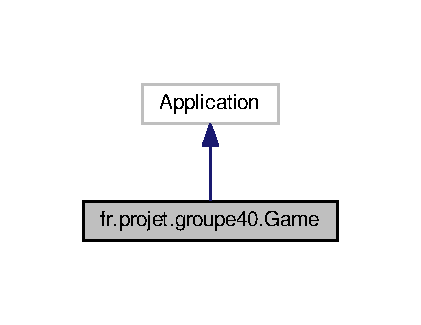
\includegraphics[width=202pt]{classfr_1_1projet_1_1groupe40_1_1_game__inherit__graph}
\end{center}
\end{figure}


Collaboration diagram for fr.\+projet.\+groupe40.\+Game\+:\nopagebreak
\begin{figure}[H]
\begin{center}
\leavevmode
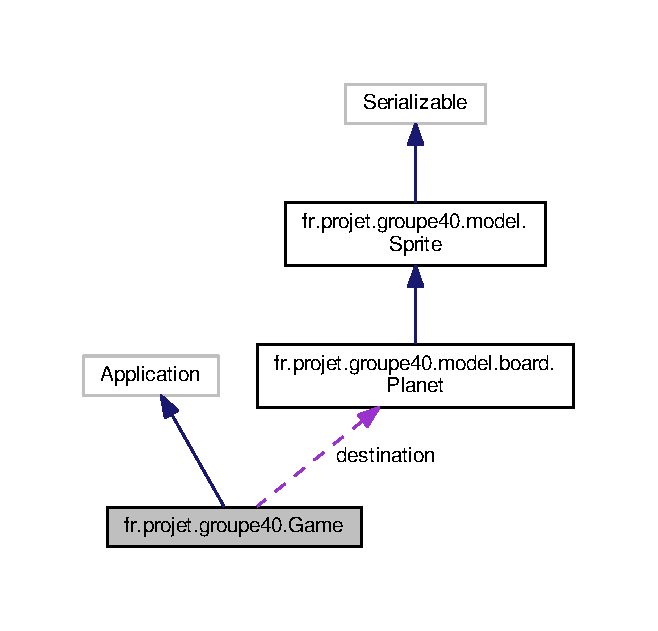
\includegraphics[width=316pt]{classfr_1_1projet_1_1groupe40_1_1_game__coll__graph}
\end{center}
\end{figure}
\subsection*{Public Member Functions}
\begin{DoxyCompactItemize}
\item 
void \hyperlink{classfr_1_1projet_1_1groupe40_1_1_game_a14c7cab9da212de8525efe1edf9ccf11}{start} (Stage stage)
\end{DoxyCompactItemize}
\subsection*{Static Public Member Functions}
\begin{DoxyCompactItemize}
\item 
static void \hyperlink{classfr_1_1projet_1_1groupe40_1_1_game_a2e45b68f672116ffe2189ff4185f0cc9}{main} (String\mbox{[}$\,$\mbox{]} args)
\end{DoxyCompactItemize}


\subsection{Member Function Documentation}
\mbox{\Hypertarget{classfr_1_1projet_1_1groupe40_1_1_game_a2e45b68f672116ffe2189ff4185f0cc9}\label{classfr_1_1projet_1_1groupe40_1_1_game_a2e45b68f672116ffe2189ff4185f0cc9}} 
\index{fr\+::projet\+::groupe40\+::\+Game@{fr\+::projet\+::groupe40\+::\+Game}!main@{main}}
\index{main@{main}!fr\+::projet\+::groupe40\+::\+Game@{fr\+::projet\+::groupe40\+::\+Game}}
\subsubsection{\texorpdfstring{main()}{main()}}
{\footnotesize\ttfamily static void fr.\+projet.\+groupe40.\+Game.\+main (\begin{DoxyParamCaption}\item[{String \mbox{[}$\,$\mbox{]}}]{args }\end{DoxyParamCaption})\hspace{0.3cm}{\ttfamily [static]}}

\mbox{\Hypertarget{classfr_1_1projet_1_1groupe40_1_1_game_a14c7cab9da212de8525efe1edf9ccf11}\label{classfr_1_1projet_1_1groupe40_1_1_game_a14c7cab9da212de8525efe1edf9ccf11}} 
\index{fr\+::projet\+::groupe40\+::\+Game@{fr\+::projet\+::groupe40\+::\+Game}!start@{start}}
\index{start@{start}!fr\+::projet\+::groupe40\+::\+Game@{fr\+::projet\+::groupe40\+::\+Game}}
\subsubsection{\texorpdfstring{start()}{start()}}
{\footnotesize\ttfamily void fr.\+projet.\+groupe40.\+Game.\+start (\begin{DoxyParamCaption}\item[{Stage}]{stage }\end{DoxyParamCaption})}

Window and game kernel creation

Saver

Rendering 

The documentation for this class was generated from the following file\+:\begin{DoxyCompactItemize}
\item 
src/fr/projet/groupe40/\hyperlink{_game_8java}{Game.\+java}\end{DoxyCompactItemize}

\hypertarget{classfr_1_1projet_1_1groupe40_1_1client_1_1handler_1_1_interaction_handler}{}\section{fr.\+projet.\+groupe40.\+client.\+handler.\+Interaction\+Handler Class Reference}
\label{classfr_1_1projet_1_1groupe40_1_1client_1_1handler_1_1_interaction_handler}\index{fr.\+projet.\+groupe40.\+client.\+handler.\+Interaction\+Handler@{fr.\+projet.\+groupe40.\+client.\+handler.\+Interaction\+Handler}}


Collaboration diagram for fr.\+projet.\+groupe40.\+client.\+handler.\+Interaction\+Handler\+:\nopagebreak
\begin{figure}[H]
\begin{center}
\leavevmode
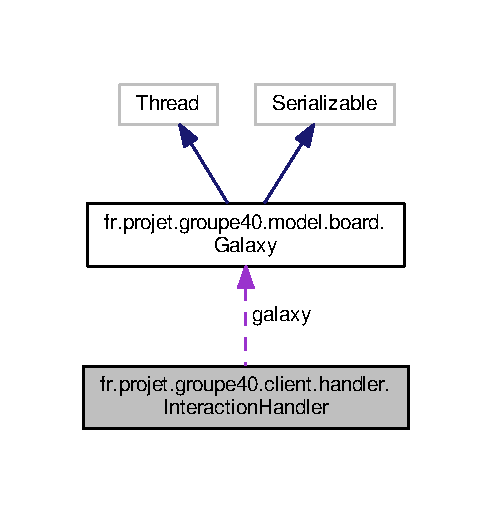
\includegraphics[width=236pt]{classfr_1_1projet_1_1groupe40_1_1client_1_1handler_1_1_interaction_handler__coll__graph}
\end{center}
\end{figure}
\subsection*{Public Member Functions}
\begin{DoxyCompactItemize}
\item 
\hyperlink{classfr_1_1projet_1_1groupe40_1_1client_1_1handler_1_1_interaction_handler_ac96a2cd52735f00717946ce4dae14c8a}{Interaction\+Handler} (\hyperlink{classfr_1_1projet_1_1groupe40_1_1model_1_1board_1_1_galaxy}{Galaxy} \hyperlink{classfr_1_1projet_1_1groupe40_1_1client_1_1handler_1_1_interaction_handler_a9cd8c67ac423a8a189cab902b148d934}{galaxy})
\item 
Event\+Handler$<$ Mouse\+Event $>$ \hyperlink{classfr_1_1projet_1_1groupe40_1_1client_1_1handler_1_1_interaction_handler_a65263a2e0561048e0d61acdddd55bd60}{get\+Mouse\+Pressed\+Event} ()
\item 
void \hyperlink{classfr_1_1projet_1_1groupe40_1_1client_1_1handler_1_1_interaction_handler_a04841979734da48633001c04b58c3570}{set\+Mouse\+Pressed\+Event} (Event\+Handler$<$ Mouse\+Event $>$ mouse\+Pressed\+Event)
\item 
Event\+Handler$<$ Mouse\+Event $>$ \hyperlink{classfr_1_1projet_1_1groupe40_1_1client_1_1handler_1_1_interaction_handler_a2d7a12f00289cacc345fed414a8aba71}{get\+Mouse\+Dragged\+Event} ()
\item 
void \hyperlink{classfr_1_1projet_1_1groupe40_1_1client_1_1handler_1_1_interaction_handler_a3d0a343f074cd2157863dbe47f786bf4}{set\+Mouse\+Dragged\+Event} (Event\+Handler$<$ Mouse\+Event $>$ mouse\+Dragged\+Event)
\item 
Event\+Handler$<$ Scroll\+Event $>$ \hyperlink{classfr_1_1projet_1_1groupe40_1_1client_1_1handler_1_1_interaction_handler_ad769e73c52ae29a54bfd6ee722fe4b1a}{get\+Scroll\+Event} ()
\item 
void \hyperlink{classfr_1_1projet_1_1groupe40_1_1client_1_1handler_1_1_interaction_handler_ad245d4139bc2ee3ea391d3709e2424f7}{set\+Scroll\+Event} (Event\+Handler$<$ Scroll\+Event $>$ scroll\+Event)
\item 
\hyperlink{classfr_1_1projet_1_1groupe40_1_1model_1_1board_1_1_galaxy}{Galaxy} \hyperlink{classfr_1_1projet_1_1groupe40_1_1client_1_1handler_1_1_interaction_handler_a92adf9509602623b1ff83accf6fcfd60}{get\+Galaxy} ()
\item 
void \hyperlink{classfr_1_1projet_1_1groupe40_1_1client_1_1handler_1_1_interaction_handler_a05733f4c93283eb97220d7f31fd38c3d}{set\+Galaxy} (\hyperlink{classfr_1_1projet_1_1groupe40_1_1model_1_1board_1_1_galaxy}{Galaxy} \hyperlink{classfr_1_1projet_1_1groupe40_1_1client_1_1handler_1_1_interaction_handler_a9cd8c67ac423a8a189cab902b148d934}{galaxy})
\end{DoxyCompactItemize}
\subsection*{Protected Attributes}
\begin{DoxyCompactItemize}
\item 
\hyperlink{classfr_1_1projet_1_1groupe40_1_1model_1_1board_1_1_galaxy}{Galaxy} \hyperlink{classfr_1_1projet_1_1groupe40_1_1client_1_1handler_1_1_interaction_handler_a9cd8c67ac423a8a189cab902b148d934}{galaxy}
\end{DoxyCompactItemize}


\subsection{Constructor \& Destructor Documentation}
\mbox{\Hypertarget{classfr_1_1projet_1_1groupe40_1_1client_1_1handler_1_1_interaction_handler_ac96a2cd52735f00717946ce4dae14c8a}\label{classfr_1_1projet_1_1groupe40_1_1client_1_1handler_1_1_interaction_handler_ac96a2cd52735f00717946ce4dae14c8a}} 
\index{fr\+::projet\+::groupe40\+::client\+::handler\+::\+Interaction\+Handler@{fr\+::projet\+::groupe40\+::client\+::handler\+::\+Interaction\+Handler}!Interaction\+Handler@{Interaction\+Handler}}
\index{Interaction\+Handler@{Interaction\+Handler}!fr\+::projet\+::groupe40\+::client\+::handler\+::\+Interaction\+Handler@{fr\+::projet\+::groupe40\+::client\+::handler\+::\+Interaction\+Handler}}
\subsubsection{\texorpdfstring{Interaction\+Handler()}{InteractionHandler()}}
{\footnotesize\ttfamily fr.\+projet.\+groupe40.\+client.\+handler.\+Interaction\+Handler.\+Interaction\+Handler (\begin{DoxyParamCaption}\item[{\hyperlink{classfr_1_1projet_1_1groupe40_1_1model_1_1board_1_1_galaxy}{Galaxy}}]{galaxy }\end{DoxyParamCaption})}



\subsection{Member Function Documentation}
\mbox{\Hypertarget{classfr_1_1projet_1_1groupe40_1_1client_1_1handler_1_1_interaction_handler_a92adf9509602623b1ff83accf6fcfd60}\label{classfr_1_1projet_1_1groupe40_1_1client_1_1handler_1_1_interaction_handler_a92adf9509602623b1ff83accf6fcfd60}} 
\index{fr\+::projet\+::groupe40\+::client\+::handler\+::\+Interaction\+Handler@{fr\+::projet\+::groupe40\+::client\+::handler\+::\+Interaction\+Handler}!get\+Galaxy@{get\+Galaxy}}
\index{get\+Galaxy@{get\+Galaxy}!fr\+::projet\+::groupe40\+::client\+::handler\+::\+Interaction\+Handler@{fr\+::projet\+::groupe40\+::client\+::handler\+::\+Interaction\+Handler}}
\subsubsection{\texorpdfstring{get\+Galaxy()}{getGalaxy()}}
{\footnotesize\ttfamily \hyperlink{classfr_1_1projet_1_1groupe40_1_1model_1_1board_1_1_galaxy}{Galaxy} fr.\+projet.\+groupe40.\+client.\+handler.\+Interaction\+Handler.\+get\+Galaxy (\begin{DoxyParamCaption}{ }\end{DoxyParamCaption})}

\mbox{\Hypertarget{classfr_1_1projet_1_1groupe40_1_1client_1_1handler_1_1_interaction_handler_a2d7a12f00289cacc345fed414a8aba71}\label{classfr_1_1projet_1_1groupe40_1_1client_1_1handler_1_1_interaction_handler_a2d7a12f00289cacc345fed414a8aba71}} 
\index{fr\+::projet\+::groupe40\+::client\+::handler\+::\+Interaction\+Handler@{fr\+::projet\+::groupe40\+::client\+::handler\+::\+Interaction\+Handler}!get\+Mouse\+Dragged\+Event@{get\+Mouse\+Dragged\+Event}}
\index{get\+Mouse\+Dragged\+Event@{get\+Mouse\+Dragged\+Event}!fr\+::projet\+::groupe40\+::client\+::handler\+::\+Interaction\+Handler@{fr\+::projet\+::groupe40\+::client\+::handler\+::\+Interaction\+Handler}}
\subsubsection{\texorpdfstring{get\+Mouse\+Dragged\+Event()}{getMouseDraggedEvent()}}
{\footnotesize\ttfamily Event\+Handler$<$Mouse\+Event$>$ fr.\+projet.\+groupe40.\+client.\+handler.\+Interaction\+Handler.\+get\+Mouse\+Dragged\+Event (\begin{DoxyParamCaption}{ }\end{DoxyParamCaption})}

\mbox{\Hypertarget{classfr_1_1projet_1_1groupe40_1_1client_1_1handler_1_1_interaction_handler_a65263a2e0561048e0d61acdddd55bd60}\label{classfr_1_1projet_1_1groupe40_1_1client_1_1handler_1_1_interaction_handler_a65263a2e0561048e0d61acdddd55bd60}} 
\index{fr\+::projet\+::groupe40\+::client\+::handler\+::\+Interaction\+Handler@{fr\+::projet\+::groupe40\+::client\+::handler\+::\+Interaction\+Handler}!get\+Mouse\+Pressed\+Event@{get\+Mouse\+Pressed\+Event}}
\index{get\+Mouse\+Pressed\+Event@{get\+Mouse\+Pressed\+Event}!fr\+::projet\+::groupe40\+::client\+::handler\+::\+Interaction\+Handler@{fr\+::projet\+::groupe40\+::client\+::handler\+::\+Interaction\+Handler}}
\subsubsection{\texorpdfstring{get\+Mouse\+Pressed\+Event()}{getMousePressedEvent()}}
{\footnotesize\ttfamily Event\+Handler$<$Mouse\+Event$>$ fr.\+projet.\+groupe40.\+client.\+handler.\+Interaction\+Handler.\+get\+Mouse\+Pressed\+Event (\begin{DoxyParamCaption}{ }\end{DoxyParamCaption})}

\mbox{\Hypertarget{classfr_1_1projet_1_1groupe40_1_1client_1_1handler_1_1_interaction_handler_ad769e73c52ae29a54bfd6ee722fe4b1a}\label{classfr_1_1projet_1_1groupe40_1_1client_1_1handler_1_1_interaction_handler_ad769e73c52ae29a54bfd6ee722fe4b1a}} 
\index{fr\+::projet\+::groupe40\+::client\+::handler\+::\+Interaction\+Handler@{fr\+::projet\+::groupe40\+::client\+::handler\+::\+Interaction\+Handler}!get\+Scroll\+Event@{get\+Scroll\+Event}}
\index{get\+Scroll\+Event@{get\+Scroll\+Event}!fr\+::projet\+::groupe40\+::client\+::handler\+::\+Interaction\+Handler@{fr\+::projet\+::groupe40\+::client\+::handler\+::\+Interaction\+Handler}}
\subsubsection{\texorpdfstring{get\+Scroll\+Event()}{getScrollEvent()}}
{\footnotesize\ttfamily Event\+Handler$<$Scroll\+Event$>$ fr.\+projet.\+groupe40.\+client.\+handler.\+Interaction\+Handler.\+get\+Scroll\+Event (\begin{DoxyParamCaption}{ }\end{DoxyParamCaption})}

\mbox{\Hypertarget{classfr_1_1projet_1_1groupe40_1_1client_1_1handler_1_1_interaction_handler_a05733f4c93283eb97220d7f31fd38c3d}\label{classfr_1_1projet_1_1groupe40_1_1client_1_1handler_1_1_interaction_handler_a05733f4c93283eb97220d7f31fd38c3d}} 
\index{fr\+::projet\+::groupe40\+::client\+::handler\+::\+Interaction\+Handler@{fr\+::projet\+::groupe40\+::client\+::handler\+::\+Interaction\+Handler}!set\+Galaxy@{set\+Galaxy}}
\index{set\+Galaxy@{set\+Galaxy}!fr\+::projet\+::groupe40\+::client\+::handler\+::\+Interaction\+Handler@{fr\+::projet\+::groupe40\+::client\+::handler\+::\+Interaction\+Handler}}
\subsubsection{\texorpdfstring{set\+Galaxy()}{setGalaxy()}}
{\footnotesize\ttfamily void fr.\+projet.\+groupe40.\+client.\+handler.\+Interaction\+Handler.\+set\+Galaxy (\begin{DoxyParamCaption}\item[{\hyperlink{classfr_1_1projet_1_1groupe40_1_1model_1_1board_1_1_galaxy}{Galaxy}}]{galaxy }\end{DoxyParamCaption})}

\mbox{\Hypertarget{classfr_1_1projet_1_1groupe40_1_1client_1_1handler_1_1_interaction_handler_a3d0a343f074cd2157863dbe47f786bf4}\label{classfr_1_1projet_1_1groupe40_1_1client_1_1handler_1_1_interaction_handler_a3d0a343f074cd2157863dbe47f786bf4}} 
\index{fr\+::projet\+::groupe40\+::client\+::handler\+::\+Interaction\+Handler@{fr\+::projet\+::groupe40\+::client\+::handler\+::\+Interaction\+Handler}!set\+Mouse\+Dragged\+Event@{set\+Mouse\+Dragged\+Event}}
\index{set\+Mouse\+Dragged\+Event@{set\+Mouse\+Dragged\+Event}!fr\+::projet\+::groupe40\+::client\+::handler\+::\+Interaction\+Handler@{fr\+::projet\+::groupe40\+::client\+::handler\+::\+Interaction\+Handler}}
\subsubsection{\texorpdfstring{set\+Mouse\+Dragged\+Event()}{setMouseDraggedEvent()}}
{\footnotesize\ttfamily void fr.\+projet.\+groupe40.\+client.\+handler.\+Interaction\+Handler.\+set\+Mouse\+Dragged\+Event (\begin{DoxyParamCaption}\item[{Event\+Handler$<$ Mouse\+Event $>$}]{mouse\+Dragged\+Event }\end{DoxyParamCaption})}

\mbox{\Hypertarget{classfr_1_1projet_1_1groupe40_1_1client_1_1handler_1_1_interaction_handler_a04841979734da48633001c04b58c3570}\label{classfr_1_1projet_1_1groupe40_1_1client_1_1handler_1_1_interaction_handler_a04841979734da48633001c04b58c3570}} 
\index{fr\+::projet\+::groupe40\+::client\+::handler\+::\+Interaction\+Handler@{fr\+::projet\+::groupe40\+::client\+::handler\+::\+Interaction\+Handler}!set\+Mouse\+Pressed\+Event@{set\+Mouse\+Pressed\+Event}}
\index{set\+Mouse\+Pressed\+Event@{set\+Mouse\+Pressed\+Event}!fr\+::projet\+::groupe40\+::client\+::handler\+::\+Interaction\+Handler@{fr\+::projet\+::groupe40\+::client\+::handler\+::\+Interaction\+Handler}}
\subsubsection{\texorpdfstring{set\+Mouse\+Pressed\+Event()}{setMousePressedEvent()}}
{\footnotesize\ttfamily void fr.\+projet.\+groupe40.\+client.\+handler.\+Interaction\+Handler.\+set\+Mouse\+Pressed\+Event (\begin{DoxyParamCaption}\item[{Event\+Handler$<$ Mouse\+Event $>$}]{mouse\+Pressed\+Event }\end{DoxyParamCaption})}

\mbox{\Hypertarget{classfr_1_1projet_1_1groupe40_1_1client_1_1handler_1_1_interaction_handler_ad245d4139bc2ee3ea391d3709e2424f7}\label{classfr_1_1projet_1_1groupe40_1_1client_1_1handler_1_1_interaction_handler_ad245d4139bc2ee3ea391d3709e2424f7}} 
\index{fr\+::projet\+::groupe40\+::client\+::handler\+::\+Interaction\+Handler@{fr\+::projet\+::groupe40\+::client\+::handler\+::\+Interaction\+Handler}!set\+Scroll\+Event@{set\+Scroll\+Event}}
\index{set\+Scroll\+Event@{set\+Scroll\+Event}!fr\+::projet\+::groupe40\+::client\+::handler\+::\+Interaction\+Handler@{fr\+::projet\+::groupe40\+::client\+::handler\+::\+Interaction\+Handler}}
\subsubsection{\texorpdfstring{set\+Scroll\+Event()}{setScrollEvent()}}
{\footnotesize\ttfamily void fr.\+projet.\+groupe40.\+client.\+handler.\+Interaction\+Handler.\+set\+Scroll\+Event (\begin{DoxyParamCaption}\item[{Event\+Handler$<$ Scroll\+Event $>$}]{scroll\+Event }\end{DoxyParamCaption})}



\subsection{Member Data Documentation}
\mbox{\Hypertarget{classfr_1_1projet_1_1groupe40_1_1client_1_1handler_1_1_interaction_handler_a9cd8c67ac423a8a189cab902b148d934}\label{classfr_1_1projet_1_1groupe40_1_1client_1_1handler_1_1_interaction_handler_a9cd8c67ac423a8a189cab902b148d934}} 
\index{fr\+::projet\+::groupe40\+::client\+::handler\+::\+Interaction\+Handler@{fr\+::projet\+::groupe40\+::client\+::handler\+::\+Interaction\+Handler}!galaxy@{galaxy}}
\index{galaxy@{galaxy}!fr\+::projet\+::groupe40\+::client\+::handler\+::\+Interaction\+Handler@{fr\+::projet\+::groupe40\+::client\+::handler\+::\+Interaction\+Handler}}
\subsubsection{\texorpdfstring{galaxy}{galaxy}}
{\footnotesize\ttfamily \hyperlink{classfr_1_1projet_1_1groupe40_1_1model_1_1board_1_1_galaxy}{Galaxy} fr.\+projet.\+groupe40.\+client.\+handler.\+Interaction\+Handler.\+galaxy\hspace{0.3cm}{\ttfamily [protected]}}



The documentation for this class was generated from the following file\+:\begin{DoxyCompactItemize}
\item 
src/fr/projet/groupe40/client/handler/\hyperlink{_interaction_handler_8java}{Interaction\+Handler.\+java}\end{DoxyCompactItemize}

\hypertarget{classfr_1_1projet_1_1groupe40_1_1client_1_1handler_1_1_keyboard_handler}{}\section{fr.\+projet.\+groupe40.\+client.\+handler.\+Keyboard\+Handler Class Reference}
\label{classfr_1_1projet_1_1groupe40_1_1client_1_1handler_1_1_keyboard_handler}\index{fr.\+projet.\+groupe40.\+client.\+handler.\+Keyboard\+Handler@{fr.\+projet.\+groupe40.\+client.\+handler.\+Keyboard\+Handler}}


The documentation for this class was generated from the following file\+:\begin{DoxyCompactItemize}
\item 
src/fr/projet/groupe40/client/handler/\hyperlink{_keyboard_handler_8java}{Keyboard\+Handler.\+java}\end{DoxyCompactItemize}

\hypertarget{classfr_1_1projet_1_1groupe40_1_1window_1_1_loading_screen}{}\section{fr.\+projet.\+groupe40.\+window.\+Loading\+Screen Class Reference}
\label{classfr_1_1projet_1_1groupe40_1_1window_1_1_loading_screen}\index{fr.\+projet.\+groupe40.\+window.\+Loading\+Screen@{fr.\+projet.\+groupe40.\+window.\+Loading\+Screen}}
\subsection*{Public Member Functions}
\begin{DoxyCompactItemize}
\item 
\hyperlink{classfr_1_1projet_1_1groupe40_1_1window_1_1_loading_screen_a9cdc0dc8e1f08399b011800bfdb7d0cd}{Loading\+Screen} ()
\end{DoxyCompactItemize}


\subsection{Constructor \& Destructor Documentation}
\mbox{\Hypertarget{classfr_1_1projet_1_1groupe40_1_1window_1_1_loading_screen_a9cdc0dc8e1f08399b011800bfdb7d0cd}\label{classfr_1_1projet_1_1groupe40_1_1window_1_1_loading_screen_a9cdc0dc8e1f08399b011800bfdb7d0cd}} 
\index{fr\+::projet\+::groupe40\+::window\+::\+Loading\+Screen@{fr\+::projet\+::groupe40\+::window\+::\+Loading\+Screen}!Loading\+Screen@{Loading\+Screen}}
\index{Loading\+Screen@{Loading\+Screen}!fr\+::projet\+::groupe40\+::window\+::\+Loading\+Screen@{fr\+::projet\+::groupe40\+::window\+::\+Loading\+Screen}}
\subsubsection{\texorpdfstring{Loading\+Screen()}{LoadingScreen()}}
{\footnotesize\ttfamily fr.\+projet.\+groupe40.\+window.\+Loading\+Screen.\+Loading\+Screen (\begin{DoxyParamCaption}{ }\end{DoxyParamCaption})}



The documentation for this class was generated from the following file\+:\begin{DoxyCompactItemize}
\item 
src/fr/projet/groupe40/window/\hyperlink{_loading_screen_8java}{Loading\+Screen.\+java}\end{DoxyCompactItemize}

\hypertarget{classfr_1_1projet_1_1groupe40_1_1window_1_1_main_menu}{}\section{fr.\+projet.\+groupe40.\+window.\+Main\+Menu Class Reference}
\label{classfr_1_1projet_1_1groupe40_1_1window_1_1_main_menu}\index{fr.\+projet.\+groupe40.\+window.\+Main\+Menu@{fr.\+projet.\+groupe40.\+window.\+Main\+Menu}}
\subsection*{Public Member Functions}
\begin{DoxyCompactItemize}
\item 
\hyperlink{classfr_1_1projet_1_1groupe40_1_1window_1_1_main_menu_a7f6750d8762abddecd2b099019a03de4}{Main\+Menu} ()
\end{DoxyCompactItemize}


\subsection{Constructor \& Destructor Documentation}
\mbox{\Hypertarget{classfr_1_1projet_1_1groupe40_1_1window_1_1_main_menu_a7f6750d8762abddecd2b099019a03de4}\label{classfr_1_1projet_1_1groupe40_1_1window_1_1_main_menu_a7f6750d8762abddecd2b099019a03de4}} 
\index{fr\+::projet\+::groupe40\+::window\+::\+Main\+Menu@{fr\+::projet\+::groupe40\+::window\+::\+Main\+Menu}!Main\+Menu@{Main\+Menu}}
\index{Main\+Menu@{Main\+Menu}!fr\+::projet\+::groupe40\+::window\+::\+Main\+Menu@{fr\+::projet\+::groupe40\+::window\+::\+Main\+Menu}}
\subsubsection{\texorpdfstring{Main\+Menu()}{MainMenu()}}
{\footnotesize\ttfamily fr.\+projet.\+groupe40.\+window.\+Main\+Menu.\+Main\+Menu (\begin{DoxyParamCaption}{ }\end{DoxyParamCaption})}



The documentation for this class was generated from the following file\+:\begin{DoxyCompactItemize}
\item 
src/fr/projet/groupe40/window/\hyperlink{_main_menu_8java}{Main\+Menu.\+java}\end{DoxyCompactItemize}

\hypertarget{classfr_1_1projet_1_1groupe40_1_1client_1_1handler_1_1_mouse_handler}{}\section{fr.\+projet.\+groupe40.\+client.\+handler.\+Mouse\+Handler Class Reference}
\label{classfr_1_1projet_1_1groupe40_1_1client_1_1handler_1_1_mouse_handler}\index{fr.\+projet.\+groupe40.\+client.\+handler.\+Mouse\+Handler@{fr.\+projet.\+groupe40.\+client.\+handler.\+Mouse\+Handler}}


The documentation for this class was generated from the following file\+:\begin{DoxyCompactItemize}
\item 
src/fr/projet/groupe40/client/handler/\hyperlink{_mouse_handler_8java}{Mouse\+Handler.\+java}\end{DoxyCompactItemize}

\hypertarget{classfr_1_1projet_1_1groupe40_1_1events_1_1_pirate_assault}{}\section{fr.\+projet.\+groupe40.\+events.\+Pirate\+Assault Class Reference}
\label{classfr_1_1projet_1_1groupe40_1_1events_1_1_pirate_assault}\index{fr.\+projet.\+groupe40.\+events.\+Pirate\+Assault@{fr.\+projet.\+groupe40.\+events.\+Pirate\+Assault}}


The documentation for this class was generated from the following file\+:\begin{DoxyCompactItemize}
\item 
src/fr/projet/groupe40/events/\hyperlink{_pirate_assault_8java}{Pirate\+Assault.\+java}\end{DoxyCompactItemize}

\hypertarget{classfr_1_1projet_1_1groupe40_1_1model_1_1board_1_1_planet}{}\section{fr.\+projet.\+groupe40.\+model.\+board.\+Planet Class Reference}
\label{classfr_1_1projet_1_1groupe40_1_1model_1_1board_1_1_planet}\index{fr.\+projet.\+groupe40.\+model.\+board.\+Planet@{fr.\+projet.\+groupe40.\+model.\+board.\+Planet}}


Inheritance diagram for fr.\+projet.\+groupe40.\+model.\+board.\+Planet\+:\nopagebreak
\begin{figure}[H]
\begin{center}
\leavevmode
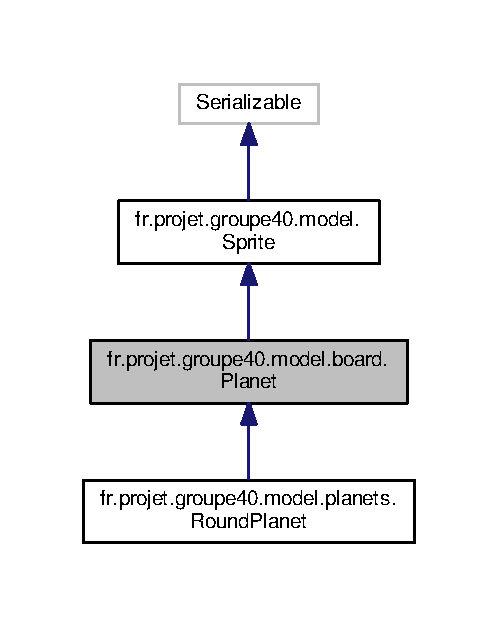
\includegraphics[width=239pt]{classfr_1_1projet_1_1groupe40_1_1model_1_1board_1_1_planet__inherit__graph}
\end{center}
\end{figure}


Collaboration diagram for fr.\+projet.\+groupe40.\+model.\+board.\+Planet\+:\nopagebreak
\begin{figure}[H]
\begin{center}
\leavevmode
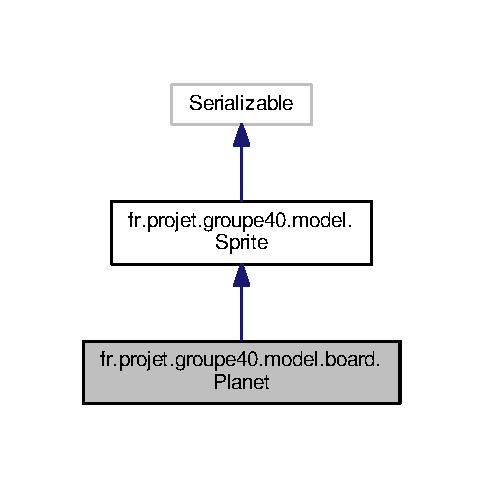
\includegraphics[width=232pt]{classfr_1_1projet_1_1groupe40_1_1model_1_1board_1_1_planet__coll__graph}
\end{center}
\end{figure}
\subsection*{Public Member Functions}
\begin{DoxyCompactItemize}
\item 
\hyperlink{classfr_1_1projet_1_1groupe40_1_1model_1_1board_1_1_planet_a14689f4495bcea6d743ba108432ce1a8}{Planet} (String path, \hyperlink{classfr_1_1projet_1_1groupe40_1_1client_1_1_user}{User} ruler, boolean is\+Planet, int x, int y)
\item 
boolean \hyperlink{classfr_1_1projet_1_1groupe40_1_1model_1_1board_1_1_planet_a89e66ac5ae9ed1186e289c51d5b84140}{clicked\+On\+Planet} (double x, double y)
\item 
void \hyperlink{classfr_1_1projet_1_1groupe40_1_1model_1_1board_1_1_planet_ab5f4d299a664ad3b73eb6c6449530fcc}{update\+Garrison} ()
\item 
void \hyperlink{classfr_1_1projet_1_1groupe40_1_1model_1_1board_1_1_planet_a971751ad9b3ed76f22c7f5e21e8d0e18}{send\+Fleet\+\_\+position} (\hyperlink{classfr_1_1projet_1_1groupe40_1_1model_1_1ships_1_1_squad}{Squad} s)
\item 
\hyperlink{classfr_1_1projet_1_1groupe40_1_1model_1_1ships_1_1_squad}{Squad} \hyperlink{classfr_1_1projet_1_1groupe40_1_1model_1_1board_1_1_planet_a84ef56833b5c5d7a4f4cbaecb2e8287f}{send\+Fleet} (\hyperlink{classfr_1_1projet_1_1groupe40_1_1model_1_1board_1_1_planet}{Planet} destination)
\item 
\hyperlink{classfr_1_1projet_1_1groupe40_1_1model_1_1ships_1_1_squad}{Squad} \hyperlink{classfr_1_1projet_1_1groupe40_1_1model_1_1board_1_1_planet_a66902570652946640bd36f78ec2a3038}{send\+Fleet} (\hyperlink{classfr_1_1projet_1_1groupe40_1_1model_1_1board_1_1_planet}{Planet} destination, double percent)
\item 
int \hyperlink{classfr_1_1projet_1_1groupe40_1_1model_1_1board_1_1_planet_a112910341d9f36d240ca4dbe961ba5fa}{calculate\+Next\+Position} ()
\item 
int \hyperlink{classfr_1_1projet_1_1groupe40_1_1model_1_1board_1_1_planet_a6964d033e72c629b179e917e0e0af896}{update\+Planete\+Position} ()
\item 
String \hyperlink{classfr_1_1projet_1_1groupe40_1_1model_1_1board_1_1_planet_adcf992792e929522ab2f15dc1eed7896}{to\+String} ()
\item 
int \hyperlink{classfr_1_1projet_1_1groupe40_1_1model_1_1board_1_1_planet_a1cc71a77c0d00ca3dca08e3789791f5d}{get\+Produce\+\_\+rate} ()
\item 
void \hyperlink{classfr_1_1projet_1_1groupe40_1_1model_1_1board_1_1_planet_a6b556f628701ec94887fbe856bc3b609}{set\+Produce\+\_\+rate} (int produce\+\_\+rate)
\item 
int \hyperlink{classfr_1_1projet_1_1groupe40_1_1model_1_1board_1_1_planet_a0f02d5be191e9d4390b6fe128197242a}{get\+Troups} ()
\item 
void \hyperlink{classfr_1_1projet_1_1groupe40_1_1model_1_1board_1_1_planet_a2412d66ee3f606d0fce1a54e7675782e}{set\+Troups} (int troups)
\item 
\hyperlink{classfr_1_1projet_1_1groupe40_1_1model_1_1ships_1_1_ship}{Ship} \hyperlink{classfr_1_1projet_1_1groupe40_1_1model_1_1board_1_1_planet_aa4fb6530a1c24adfc94218411840a65a}{get\+Ships\+\_\+type} ()
\item 
void \hyperlink{classfr_1_1projet_1_1groupe40_1_1model_1_1board_1_1_planet_a3d96bcb39bd1e5b3ab175dd5dcbd6d1f}{set\+Ships\+\_\+type} (\hyperlink{classfr_1_1projet_1_1groupe40_1_1model_1_1ships_1_1_ship}{Ship} ships\+\_\+type)
\item 
boolean \hyperlink{classfr_1_1projet_1_1groupe40_1_1model_1_1board_1_1_planet_ace2894a752d167330eab0642eb429cd6}{is\+Selected} ()
\item 
void \hyperlink{classfr_1_1projet_1_1groupe40_1_1model_1_1board_1_1_planet_a83902887fd1e26cc74b75da893cf5d90}{set\+Selected} (boolean selected)
\end{DoxyCompactItemize}


\subsection{Constructor \& Destructor Documentation}
\mbox{\Hypertarget{classfr_1_1projet_1_1groupe40_1_1model_1_1board_1_1_planet_a14689f4495bcea6d743ba108432ce1a8}\label{classfr_1_1projet_1_1groupe40_1_1model_1_1board_1_1_planet_a14689f4495bcea6d743ba108432ce1a8}} 
\index{fr\+::projet\+::groupe40\+::model\+::board\+::\+Planet@{fr\+::projet\+::groupe40\+::model\+::board\+::\+Planet}!Planet@{Planet}}
\index{Planet@{Planet}!fr\+::projet\+::groupe40\+::model\+::board\+::\+Planet@{fr\+::projet\+::groupe40\+::model\+::board\+::\+Planet}}
\subsubsection{\texorpdfstring{Planet()}{Planet()}}
{\footnotesize\ttfamily fr.\+projet.\+groupe40.\+model.\+board.\+Planet.\+Planet (\begin{DoxyParamCaption}\item[{String}]{path,  }\item[{\hyperlink{classfr_1_1projet_1_1groupe40_1_1client_1_1_user}{User}}]{ruler,  }\item[{boolean}]{is\+Planet,  }\item[{int}]{x,  }\item[{int}]{y }\end{DoxyParamCaption})}



\subsection{Member Function Documentation}
\mbox{\Hypertarget{classfr_1_1projet_1_1groupe40_1_1model_1_1board_1_1_planet_a112910341d9f36d240ca4dbe961ba5fa}\label{classfr_1_1projet_1_1groupe40_1_1model_1_1board_1_1_planet_a112910341d9f36d240ca4dbe961ba5fa}} 
\index{fr\+::projet\+::groupe40\+::model\+::board\+::\+Planet@{fr\+::projet\+::groupe40\+::model\+::board\+::\+Planet}!calculate\+Next\+Position@{calculate\+Next\+Position}}
\index{calculate\+Next\+Position@{calculate\+Next\+Position}!fr\+::projet\+::groupe40\+::model\+::board\+::\+Planet@{fr\+::projet\+::groupe40\+::model\+::board\+::\+Planet}}
\subsubsection{\texorpdfstring{calculate\+Next\+Position()}{calculateNextPosition()}}
{\footnotesize\ttfamily int fr.\+projet.\+groupe40.\+model.\+board.\+Planet.\+calculate\+Next\+Position (\begin{DoxyParamCaption}{ }\end{DoxyParamCaption})}

\mbox{\Hypertarget{classfr_1_1projet_1_1groupe40_1_1model_1_1board_1_1_planet_a89e66ac5ae9ed1186e289c51d5b84140}\label{classfr_1_1projet_1_1groupe40_1_1model_1_1board_1_1_planet_a89e66ac5ae9ed1186e289c51d5b84140}} 
\index{fr\+::projet\+::groupe40\+::model\+::board\+::\+Planet@{fr\+::projet\+::groupe40\+::model\+::board\+::\+Planet}!clicked\+On\+Planet@{clicked\+On\+Planet}}
\index{clicked\+On\+Planet@{clicked\+On\+Planet}!fr\+::projet\+::groupe40\+::model\+::board\+::\+Planet@{fr\+::projet\+::groupe40\+::model\+::board\+::\+Planet}}
\subsubsection{\texorpdfstring{clicked\+On\+Planet()}{clickedOnPlanet()}}
{\footnotesize\ttfamily boolean fr.\+projet.\+groupe40.\+model.\+board.\+Planet.\+clicked\+On\+Planet (\begin{DoxyParamCaption}\item[{double}]{x,  }\item[{double}]{y }\end{DoxyParamCaption})}

Utilities \mbox{\Hypertarget{classfr_1_1projet_1_1groupe40_1_1model_1_1board_1_1_planet_a1cc71a77c0d00ca3dca08e3789791f5d}\label{classfr_1_1projet_1_1groupe40_1_1model_1_1board_1_1_planet_a1cc71a77c0d00ca3dca08e3789791f5d}} 
\index{fr\+::projet\+::groupe40\+::model\+::board\+::\+Planet@{fr\+::projet\+::groupe40\+::model\+::board\+::\+Planet}!get\+Produce\+\_\+rate@{get\+Produce\+\_\+rate}}
\index{get\+Produce\+\_\+rate@{get\+Produce\+\_\+rate}!fr\+::projet\+::groupe40\+::model\+::board\+::\+Planet@{fr\+::projet\+::groupe40\+::model\+::board\+::\+Planet}}
\subsubsection{\texorpdfstring{get\+Produce\+\_\+rate()}{getProduce\_rate()}}
{\footnotesize\ttfamily int fr.\+projet.\+groupe40.\+model.\+board.\+Planet.\+get\+Produce\+\_\+rate (\begin{DoxyParamCaption}{ }\end{DoxyParamCaption})}

\mbox{\Hypertarget{classfr_1_1projet_1_1groupe40_1_1model_1_1board_1_1_planet_aa4fb6530a1c24adfc94218411840a65a}\label{classfr_1_1projet_1_1groupe40_1_1model_1_1board_1_1_planet_aa4fb6530a1c24adfc94218411840a65a}} 
\index{fr\+::projet\+::groupe40\+::model\+::board\+::\+Planet@{fr\+::projet\+::groupe40\+::model\+::board\+::\+Planet}!get\+Ships\+\_\+type@{get\+Ships\+\_\+type}}
\index{get\+Ships\+\_\+type@{get\+Ships\+\_\+type}!fr\+::projet\+::groupe40\+::model\+::board\+::\+Planet@{fr\+::projet\+::groupe40\+::model\+::board\+::\+Planet}}
\subsubsection{\texorpdfstring{get\+Ships\+\_\+type()}{getShips\_type()}}
{\footnotesize\ttfamily \hyperlink{classfr_1_1projet_1_1groupe40_1_1model_1_1ships_1_1_ship}{Ship} fr.\+projet.\+groupe40.\+model.\+board.\+Planet.\+get\+Ships\+\_\+type (\begin{DoxyParamCaption}{ }\end{DoxyParamCaption})}

\mbox{\Hypertarget{classfr_1_1projet_1_1groupe40_1_1model_1_1board_1_1_planet_a0f02d5be191e9d4390b6fe128197242a}\label{classfr_1_1projet_1_1groupe40_1_1model_1_1board_1_1_planet_a0f02d5be191e9d4390b6fe128197242a}} 
\index{fr\+::projet\+::groupe40\+::model\+::board\+::\+Planet@{fr\+::projet\+::groupe40\+::model\+::board\+::\+Planet}!get\+Troups@{get\+Troups}}
\index{get\+Troups@{get\+Troups}!fr\+::projet\+::groupe40\+::model\+::board\+::\+Planet@{fr\+::projet\+::groupe40\+::model\+::board\+::\+Planet}}
\subsubsection{\texorpdfstring{get\+Troups()}{getTroups()}}
{\footnotesize\ttfamily int fr.\+projet.\+groupe40.\+model.\+board.\+Planet.\+get\+Troups (\begin{DoxyParamCaption}{ }\end{DoxyParamCaption})}

\mbox{\Hypertarget{classfr_1_1projet_1_1groupe40_1_1model_1_1board_1_1_planet_ace2894a752d167330eab0642eb429cd6}\label{classfr_1_1projet_1_1groupe40_1_1model_1_1board_1_1_planet_ace2894a752d167330eab0642eb429cd6}} 
\index{fr\+::projet\+::groupe40\+::model\+::board\+::\+Planet@{fr\+::projet\+::groupe40\+::model\+::board\+::\+Planet}!is\+Selected@{is\+Selected}}
\index{is\+Selected@{is\+Selected}!fr\+::projet\+::groupe40\+::model\+::board\+::\+Planet@{fr\+::projet\+::groupe40\+::model\+::board\+::\+Planet}}
\subsubsection{\texorpdfstring{is\+Selected()}{isSelected()}}
{\footnotesize\ttfamily boolean fr.\+projet.\+groupe40.\+model.\+board.\+Planet.\+is\+Selected (\begin{DoxyParamCaption}{ }\end{DoxyParamCaption})}

\mbox{\Hypertarget{classfr_1_1projet_1_1groupe40_1_1model_1_1board_1_1_planet_a84ef56833b5c5d7a4f4cbaecb2e8287f}\label{classfr_1_1projet_1_1groupe40_1_1model_1_1board_1_1_planet_a84ef56833b5c5d7a4f4cbaecb2e8287f}} 
\index{fr\+::projet\+::groupe40\+::model\+::board\+::\+Planet@{fr\+::projet\+::groupe40\+::model\+::board\+::\+Planet}!send\+Fleet@{send\+Fleet}}
\index{send\+Fleet@{send\+Fleet}!fr\+::projet\+::groupe40\+::model\+::board\+::\+Planet@{fr\+::projet\+::groupe40\+::model\+::board\+::\+Planet}}
\subsubsection{\texorpdfstring{send\+Fleet()}{sendFleet()}\hspace{0.1cm}{\footnotesize\ttfamily [1/2]}}
{\footnotesize\ttfamily \hyperlink{classfr_1_1projet_1_1groupe40_1_1model_1_1ships_1_1_squad}{Squad} fr.\+projet.\+groupe40.\+model.\+board.\+Planet.\+send\+Fleet (\begin{DoxyParamCaption}\item[{\hyperlink{classfr_1_1projet_1_1groupe40_1_1model_1_1board_1_1_planet}{Planet}}]{destination }\end{DoxyParamCaption})}

\mbox{\Hypertarget{classfr_1_1projet_1_1groupe40_1_1model_1_1board_1_1_planet_a66902570652946640bd36f78ec2a3038}\label{classfr_1_1projet_1_1groupe40_1_1model_1_1board_1_1_planet_a66902570652946640bd36f78ec2a3038}} 
\index{fr\+::projet\+::groupe40\+::model\+::board\+::\+Planet@{fr\+::projet\+::groupe40\+::model\+::board\+::\+Planet}!send\+Fleet@{send\+Fleet}}
\index{send\+Fleet@{send\+Fleet}!fr\+::projet\+::groupe40\+::model\+::board\+::\+Planet@{fr\+::projet\+::groupe40\+::model\+::board\+::\+Planet}}
\subsubsection{\texorpdfstring{send\+Fleet()}{sendFleet()}\hspace{0.1cm}{\footnotesize\ttfamily [2/2]}}
{\footnotesize\ttfamily \hyperlink{classfr_1_1projet_1_1groupe40_1_1model_1_1ships_1_1_squad}{Squad} fr.\+projet.\+groupe40.\+model.\+board.\+Planet.\+send\+Fleet (\begin{DoxyParamCaption}\item[{\hyperlink{classfr_1_1projet_1_1groupe40_1_1model_1_1board_1_1_planet}{Planet}}]{destination,  }\item[{double}]{percent }\end{DoxyParamCaption})}

\mbox{\Hypertarget{classfr_1_1projet_1_1groupe40_1_1model_1_1board_1_1_planet_a971751ad9b3ed76f22c7f5e21e8d0e18}\label{classfr_1_1projet_1_1groupe40_1_1model_1_1board_1_1_planet_a971751ad9b3ed76f22c7f5e21e8d0e18}} 
\index{fr\+::projet\+::groupe40\+::model\+::board\+::\+Planet@{fr\+::projet\+::groupe40\+::model\+::board\+::\+Planet}!send\+Fleet\+\_\+position@{send\+Fleet\+\_\+position}}
\index{send\+Fleet\+\_\+position@{send\+Fleet\+\_\+position}!fr\+::projet\+::groupe40\+::model\+::board\+::\+Planet@{fr\+::projet\+::groupe40\+::model\+::board\+::\+Planet}}
\subsubsection{\texorpdfstring{send\+Fleet\+\_\+position()}{sendFleet\_position()}}
{\footnotesize\ttfamily void fr.\+projet.\+groupe40.\+model.\+board.\+Planet.\+send\+Fleet\+\_\+position (\begin{DoxyParamCaption}\item[{\hyperlink{classfr_1_1projet_1_1groupe40_1_1model_1_1ships_1_1_squad}{Squad}}]{s }\end{DoxyParamCaption})}

Interactions \mbox{\Hypertarget{classfr_1_1projet_1_1groupe40_1_1model_1_1board_1_1_planet_a6b556f628701ec94887fbe856bc3b609}\label{classfr_1_1projet_1_1groupe40_1_1model_1_1board_1_1_planet_a6b556f628701ec94887fbe856bc3b609}} 
\index{fr\+::projet\+::groupe40\+::model\+::board\+::\+Planet@{fr\+::projet\+::groupe40\+::model\+::board\+::\+Planet}!set\+Produce\+\_\+rate@{set\+Produce\+\_\+rate}}
\index{set\+Produce\+\_\+rate@{set\+Produce\+\_\+rate}!fr\+::projet\+::groupe40\+::model\+::board\+::\+Planet@{fr\+::projet\+::groupe40\+::model\+::board\+::\+Planet}}
\subsubsection{\texorpdfstring{set\+Produce\+\_\+rate()}{setProduce\_rate()}}
{\footnotesize\ttfamily void fr.\+projet.\+groupe40.\+model.\+board.\+Planet.\+set\+Produce\+\_\+rate (\begin{DoxyParamCaption}\item[{int}]{produce\+\_\+rate }\end{DoxyParamCaption})}

\mbox{\Hypertarget{classfr_1_1projet_1_1groupe40_1_1model_1_1board_1_1_planet_a83902887fd1e26cc74b75da893cf5d90}\label{classfr_1_1projet_1_1groupe40_1_1model_1_1board_1_1_planet_a83902887fd1e26cc74b75da893cf5d90}} 
\index{fr\+::projet\+::groupe40\+::model\+::board\+::\+Planet@{fr\+::projet\+::groupe40\+::model\+::board\+::\+Planet}!set\+Selected@{set\+Selected}}
\index{set\+Selected@{set\+Selected}!fr\+::projet\+::groupe40\+::model\+::board\+::\+Planet@{fr\+::projet\+::groupe40\+::model\+::board\+::\+Planet}}
\subsubsection{\texorpdfstring{set\+Selected()}{setSelected()}}
{\footnotesize\ttfamily void fr.\+projet.\+groupe40.\+model.\+board.\+Planet.\+set\+Selected (\begin{DoxyParamCaption}\item[{boolean}]{selected }\end{DoxyParamCaption})}

\mbox{\Hypertarget{classfr_1_1projet_1_1groupe40_1_1model_1_1board_1_1_planet_a3d96bcb39bd1e5b3ab175dd5dcbd6d1f}\label{classfr_1_1projet_1_1groupe40_1_1model_1_1board_1_1_planet_a3d96bcb39bd1e5b3ab175dd5dcbd6d1f}} 
\index{fr\+::projet\+::groupe40\+::model\+::board\+::\+Planet@{fr\+::projet\+::groupe40\+::model\+::board\+::\+Planet}!set\+Ships\+\_\+type@{set\+Ships\+\_\+type}}
\index{set\+Ships\+\_\+type@{set\+Ships\+\_\+type}!fr\+::projet\+::groupe40\+::model\+::board\+::\+Planet@{fr\+::projet\+::groupe40\+::model\+::board\+::\+Planet}}
\subsubsection{\texorpdfstring{set\+Ships\+\_\+type()}{setShips\_type()}}
{\footnotesize\ttfamily void fr.\+projet.\+groupe40.\+model.\+board.\+Planet.\+set\+Ships\+\_\+type (\begin{DoxyParamCaption}\item[{\hyperlink{classfr_1_1projet_1_1groupe40_1_1model_1_1ships_1_1_ship}{Ship}}]{ships\+\_\+type }\end{DoxyParamCaption})}

\mbox{\Hypertarget{classfr_1_1projet_1_1groupe40_1_1model_1_1board_1_1_planet_a2412d66ee3f606d0fce1a54e7675782e}\label{classfr_1_1projet_1_1groupe40_1_1model_1_1board_1_1_planet_a2412d66ee3f606d0fce1a54e7675782e}} 
\index{fr\+::projet\+::groupe40\+::model\+::board\+::\+Planet@{fr\+::projet\+::groupe40\+::model\+::board\+::\+Planet}!set\+Troups@{set\+Troups}}
\index{set\+Troups@{set\+Troups}!fr\+::projet\+::groupe40\+::model\+::board\+::\+Planet@{fr\+::projet\+::groupe40\+::model\+::board\+::\+Planet}}
\subsubsection{\texorpdfstring{set\+Troups()}{setTroups()}}
{\footnotesize\ttfamily void fr.\+projet.\+groupe40.\+model.\+board.\+Planet.\+set\+Troups (\begin{DoxyParamCaption}\item[{int}]{troups }\end{DoxyParamCaption})}

\mbox{\Hypertarget{classfr_1_1projet_1_1groupe40_1_1model_1_1board_1_1_planet_adcf992792e929522ab2f15dc1eed7896}\label{classfr_1_1projet_1_1groupe40_1_1model_1_1board_1_1_planet_adcf992792e929522ab2f15dc1eed7896}} 
\index{fr\+::projet\+::groupe40\+::model\+::board\+::\+Planet@{fr\+::projet\+::groupe40\+::model\+::board\+::\+Planet}!to\+String@{to\+String}}
\index{to\+String@{to\+String}!fr\+::projet\+::groupe40\+::model\+::board\+::\+Planet@{fr\+::projet\+::groupe40\+::model\+::board\+::\+Planet}}
\subsubsection{\texorpdfstring{to\+String()}{toString()}}
{\footnotesize\ttfamily String fr.\+projet.\+groupe40.\+model.\+board.\+Planet.\+to\+String (\begin{DoxyParamCaption}{ }\end{DoxyParamCaption})}

\mbox{\Hypertarget{classfr_1_1projet_1_1groupe40_1_1model_1_1board_1_1_planet_ab5f4d299a664ad3b73eb6c6449530fcc}\label{classfr_1_1projet_1_1groupe40_1_1model_1_1board_1_1_planet_ab5f4d299a664ad3b73eb6c6449530fcc}} 
\index{fr\+::projet\+::groupe40\+::model\+::board\+::\+Planet@{fr\+::projet\+::groupe40\+::model\+::board\+::\+Planet}!update\+Garrison@{update\+Garrison}}
\index{update\+Garrison@{update\+Garrison}!fr\+::projet\+::groupe40\+::model\+::board\+::\+Planet@{fr\+::projet\+::groupe40\+::model\+::board\+::\+Planet}}
\subsubsection{\texorpdfstring{update\+Garrison()}{updateGarrison()}}
{\footnotesize\ttfamily void fr.\+projet.\+groupe40.\+model.\+board.\+Planet.\+update\+Garrison (\begin{DoxyParamCaption}{ }\end{DoxyParamCaption})}

Update \mbox{\Hypertarget{classfr_1_1projet_1_1groupe40_1_1model_1_1board_1_1_planet_a6964d033e72c629b179e917e0e0af896}\label{classfr_1_1projet_1_1groupe40_1_1model_1_1board_1_1_planet_a6964d033e72c629b179e917e0e0af896}} 
\index{fr\+::projet\+::groupe40\+::model\+::board\+::\+Planet@{fr\+::projet\+::groupe40\+::model\+::board\+::\+Planet}!update\+Planete\+Position@{update\+Planete\+Position}}
\index{update\+Planete\+Position@{update\+Planete\+Position}!fr\+::projet\+::groupe40\+::model\+::board\+::\+Planet@{fr\+::projet\+::groupe40\+::model\+::board\+::\+Planet}}
\subsubsection{\texorpdfstring{update\+Planete\+Position()}{updatePlanetePosition()}}
{\footnotesize\ttfamily int fr.\+projet.\+groupe40.\+model.\+board.\+Planet.\+update\+Planete\+Position (\begin{DoxyParamCaption}{ }\end{DoxyParamCaption})}



The documentation for this class was generated from the following file\+:\begin{DoxyCompactItemize}
\item 
src/fr/projet/groupe40/model/board/\hyperlink{_planet_8java}{Planet.\+java}\end{DoxyCompactItemize}

\hypertarget{classfr_1_1projet_1_1groupe40_1_1model_1_1planets_1_1_round_planet}{}\section{fr.\+projet.\+groupe40.\+model.\+planets.\+Round\+Planet Class Reference}
\label{classfr_1_1projet_1_1groupe40_1_1model_1_1planets_1_1_round_planet}\index{fr.\+projet.\+groupe40.\+model.\+planets.\+Round\+Planet@{fr.\+projet.\+groupe40.\+model.\+planets.\+Round\+Planet}}


Inheritance diagram for fr.\+projet.\+groupe40.\+model.\+planets.\+Round\+Planet\+:\nopagebreak
\begin{figure}[H]
\begin{center}
\leavevmode
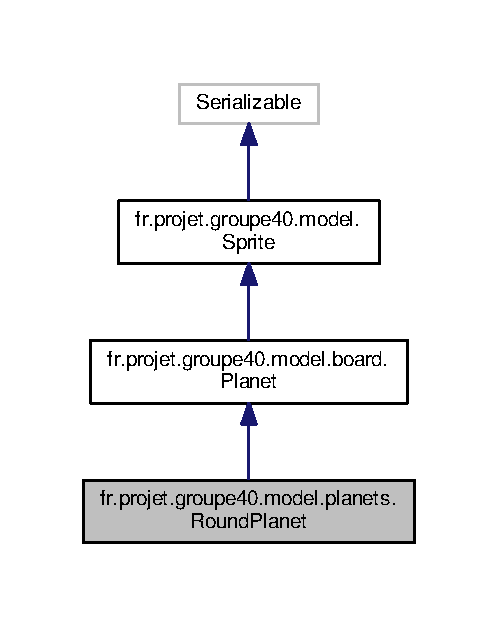
\includegraphics[width=239pt]{classfr_1_1projet_1_1groupe40_1_1model_1_1planets_1_1_round_planet__inherit__graph}
\end{center}
\end{figure}


Collaboration diagram for fr.\+projet.\+groupe40.\+model.\+planets.\+Round\+Planet\+:\nopagebreak
\begin{figure}[H]
\begin{center}
\leavevmode
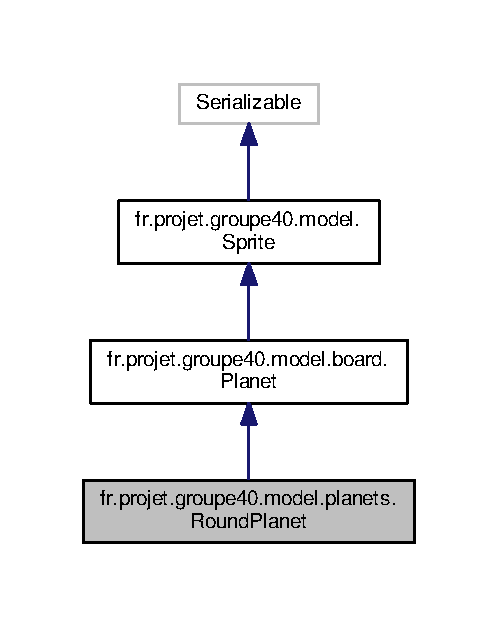
\includegraphics[width=239pt]{classfr_1_1projet_1_1groupe40_1_1model_1_1planets_1_1_round_planet__coll__graph}
\end{center}
\end{figure}
\subsection*{Public Member Functions}
\begin{DoxyCompactItemize}
\item 
\hyperlink{classfr_1_1projet_1_1groupe40_1_1model_1_1planets_1_1_round_planet_a92efe16cffdc4650d2e8b802897c940b}{Round\+Planet} (\hyperlink{classfr_1_1projet_1_1groupe40_1_1client_1_1_user}{User} ruler, boolean is\+Planet, int x, int y)
\end{DoxyCompactItemize}


\subsection{Constructor \& Destructor Documentation}
\mbox{\Hypertarget{classfr_1_1projet_1_1groupe40_1_1model_1_1planets_1_1_round_planet_a92efe16cffdc4650d2e8b802897c940b}\label{classfr_1_1projet_1_1groupe40_1_1model_1_1planets_1_1_round_planet_a92efe16cffdc4650d2e8b802897c940b}} 
\index{fr\+::projet\+::groupe40\+::model\+::planets\+::\+Round\+Planet@{fr\+::projet\+::groupe40\+::model\+::planets\+::\+Round\+Planet}!Round\+Planet@{Round\+Planet}}
\index{Round\+Planet@{Round\+Planet}!fr\+::projet\+::groupe40\+::model\+::planets\+::\+Round\+Planet@{fr\+::projet\+::groupe40\+::model\+::planets\+::\+Round\+Planet}}
\subsubsection{\texorpdfstring{Round\+Planet()}{RoundPlanet()}}
{\footnotesize\ttfamily fr.\+projet.\+groupe40.\+model.\+planets.\+Round\+Planet.\+Round\+Planet (\begin{DoxyParamCaption}\item[{\hyperlink{classfr_1_1projet_1_1groupe40_1_1client_1_1_user}{User}}]{ruler,  }\item[{boolean}]{is\+Planet,  }\item[{int}]{x,  }\item[{int}]{y }\end{DoxyParamCaption})}



The documentation for this class was generated from the following file\+:\begin{DoxyCompactItemize}
\item 
src/fr/projet/groupe40/model/planets/\hyperlink{_round_planet_8java}{Round\+Planet.\+java}\end{DoxyCompactItemize}

\hypertarget{classfr_1_1projet_1_1groupe40_1_1window_1_1_settings_menu}{}\section{fr.\+projet.\+groupe40.\+window.\+Settings\+Menu Class Reference}
\label{classfr_1_1projet_1_1groupe40_1_1window_1_1_settings_menu}\index{fr.\+projet.\+groupe40.\+window.\+Settings\+Menu@{fr.\+projet.\+groupe40.\+window.\+Settings\+Menu}}


The documentation for this class was generated from the following file\+:\begin{DoxyCompactItemize}
\item 
src/fr/projet/groupe40/window/\hyperlink{_settings_menu_8java}{Settings\+Menu.\+java}\end{DoxyCompactItemize}

\hypertarget{classfr_1_1projet_1_1groupe40_1_1model_1_1ships_1_1_ship}{}\section{fr.\+projet.\+groupe40.\+model.\+ships.\+Ship Class Reference}
\label{classfr_1_1projet_1_1groupe40_1_1model_1_1ships_1_1_ship}\index{fr.\+projet.\+groupe40.\+model.\+ships.\+Ship@{fr.\+projet.\+groupe40.\+model.\+ships.\+Ship}}


Inheritance diagram for fr.\+projet.\+groupe40.\+model.\+ships.\+Ship\+:\nopagebreak
\begin{figure}[H]
\begin{center}
\leavevmode
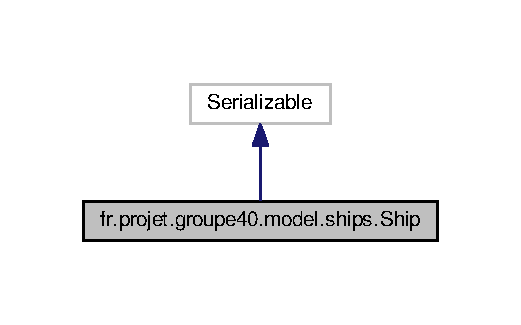
\includegraphics[width=250pt]{classfr_1_1projet_1_1groupe40_1_1model_1_1ships_1_1_ship__inherit__graph}
\end{center}
\end{figure}


Collaboration diagram for fr.\+projet.\+groupe40.\+model.\+ships.\+Ship\+:\nopagebreak
\begin{figure}[H]
\begin{center}
\leavevmode
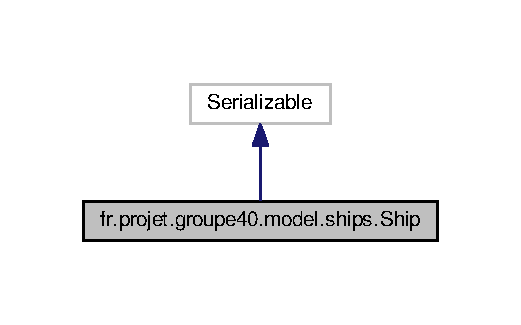
\includegraphics[width=250pt]{classfr_1_1projet_1_1groupe40_1_1model_1_1ships_1_1_ship__coll__graph}
\end{center}
\end{figure}
\subsection*{Public Member Functions}
\begin{DoxyCompactItemize}
\item 
\hyperlink{classfr_1_1projet_1_1groupe40_1_1model_1_1ships_1_1_ship_ab0ceda4452b34d91f77ecf1a3275d182}{Ship} (int speed, int power, int production\+\_\+time)
\item 
\hyperlink{classfr_1_1projet_1_1groupe40_1_1model_1_1ships_1_1_ship_a2c31827efa3141409391f989e60aca58}{Ship} ()
\item 
int \hyperlink{classfr_1_1projet_1_1groupe40_1_1model_1_1ships_1_1_ship_ac8116629f4490bf3dcac06fb43036b1c}{get\+Speed} ()
\item 
void \hyperlink{classfr_1_1projet_1_1groupe40_1_1model_1_1ships_1_1_ship_a1e9f20684a7337428f3eeba2751b3c9a}{set\+Speed} (int speed)
\item 
int \hyperlink{classfr_1_1projet_1_1groupe40_1_1model_1_1ships_1_1_ship_a1740ea91dcc786208350a3125a7acfd3}{get\+Power} ()
\item 
void \hyperlink{classfr_1_1projet_1_1groupe40_1_1model_1_1ships_1_1_ship_abdfeb45c897cf6b31d8236f9e4e881f7}{set\+Power} (int power)
\item 
int \hyperlink{classfr_1_1projet_1_1groupe40_1_1model_1_1ships_1_1_ship_af207f2465b91217a5b178b27fa2351aa}{get\+Production\+\_\+time} ()
\item 
void \hyperlink{classfr_1_1projet_1_1groupe40_1_1model_1_1ships_1_1_ship_a1d404e1bedd38ad6a347862cb518927d}{set\+Production\+\_\+time} (int production\+\_\+time)
\end{DoxyCompactItemize}


\subsection{Constructor \& Destructor Documentation}
\mbox{\Hypertarget{classfr_1_1projet_1_1groupe40_1_1model_1_1ships_1_1_ship_ab0ceda4452b34d91f77ecf1a3275d182}\label{classfr_1_1projet_1_1groupe40_1_1model_1_1ships_1_1_ship_ab0ceda4452b34d91f77ecf1a3275d182}} 
\index{fr\+::projet\+::groupe40\+::model\+::ships\+::\+Ship@{fr\+::projet\+::groupe40\+::model\+::ships\+::\+Ship}!Ship@{Ship}}
\index{Ship@{Ship}!fr\+::projet\+::groupe40\+::model\+::ships\+::\+Ship@{fr\+::projet\+::groupe40\+::model\+::ships\+::\+Ship}}
\subsubsection{\texorpdfstring{Ship()}{Ship()}\hspace{0.1cm}{\footnotesize\ttfamily [1/2]}}
{\footnotesize\ttfamily fr.\+projet.\+groupe40.\+model.\+ships.\+Ship.\+Ship (\begin{DoxyParamCaption}\item[{int}]{speed,  }\item[{int}]{power,  }\item[{int}]{production\+\_\+time }\end{DoxyParamCaption})}

\mbox{\Hypertarget{classfr_1_1projet_1_1groupe40_1_1model_1_1ships_1_1_ship_a2c31827efa3141409391f989e60aca58}\label{classfr_1_1projet_1_1groupe40_1_1model_1_1ships_1_1_ship_a2c31827efa3141409391f989e60aca58}} 
\index{fr\+::projet\+::groupe40\+::model\+::ships\+::\+Ship@{fr\+::projet\+::groupe40\+::model\+::ships\+::\+Ship}!Ship@{Ship}}
\index{Ship@{Ship}!fr\+::projet\+::groupe40\+::model\+::ships\+::\+Ship@{fr\+::projet\+::groupe40\+::model\+::ships\+::\+Ship}}
\subsubsection{\texorpdfstring{Ship()}{Ship()}\hspace{0.1cm}{\footnotesize\ttfamily [2/2]}}
{\footnotesize\ttfamily fr.\+projet.\+groupe40.\+model.\+ships.\+Ship.\+Ship (\begin{DoxyParamCaption}{ }\end{DoxyParamCaption})}



\subsection{Member Function Documentation}
\mbox{\Hypertarget{classfr_1_1projet_1_1groupe40_1_1model_1_1ships_1_1_ship_a1740ea91dcc786208350a3125a7acfd3}\label{classfr_1_1projet_1_1groupe40_1_1model_1_1ships_1_1_ship_a1740ea91dcc786208350a3125a7acfd3}} 
\index{fr\+::projet\+::groupe40\+::model\+::ships\+::\+Ship@{fr\+::projet\+::groupe40\+::model\+::ships\+::\+Ship}!get\+Power@{get\+Power}}
\index{get\+Power@{get\+Power}!fr\+::projet\+::groupe40\+::model\+::ships\+::\+Ship@{fr\+::projet\+::groupe40\+::model\+::ships\+::\+Ship}}
\subsubsection{\texorpdfstring{get\+Power()}{getPower()}}
{\footnotesize\ttfamily int fr.\+projet.\+groupe40.\+model.\+ships.\+Ship.\+get\+Power (\begin{DoxyParamCaption}{ }\end{DoxyParamCaption})}

\mbox{\Hypertarget{classfr_1_1projet_1_1groupe40_1_1model_1_1ships_1_1_ship_af207f2465b91217a5b178b27fa2351aa}\label{classfr_1_1projet_1_1groupe40_1_1model_1_1ships_1_1_ship_af207f2465b91217a5b178b27fa2351aa}} 
\index{fr\+::projet\+::groupe40\+::model\+::ships\+::\+Ship@{fr\+::projet\+::groupe40\+::model\+::ships\+::\+Ship}!get\+Production\+\_\+time@{get\+Production\+\_\+time}}
\index{get\+Production\+\_\+time@{get\+Production\+\_\+time}!fr\+::projet\+::groupe40\+::model\+::ships\+::\+Ship@{fr\+::projet\+::groupe40\+::model\+::ships\+::\+Ship}}
\subsubsection{\texorpdfstring{get\+Production\+\_\+time()}{getProduction\_time()}}
{\footnotesize\ttfamily int fr.\+projet.\+groupe40.\+model.\+ships.\+Ship.\+get\+Production\+\_\+time (\begin{DoxyParamCaption}{ }\end{DoxyParamCaption})}

\mbox{\Hypertarget{classfr_1_1projet_1_1groupe40_1_1model_1_1ships_1_1_ship_ac8116629f4490bf3dcac06fb43036b1c}\label{classfr_1_1projet_1_1groupe40_1_1model_1_1ships_1_1_ship_ac8116629f4490bf3dcac06fb43036b1c}} 
\index{fr\+::projet\+::groupe40\+::model\+::ships\+::\+Ship@{fr\+::projet\+::groupe40\+::model\+::ships\+::\+Ship}!get\+Speed@{get\+Speed}}
\index{get\+Speed@{get\+Speed}!fr\+::projet\+::groupe40\+::model\+::ships\+::\+Ship@{fr\+::projet\+::groupe40\+::model\+::ships\+::\+Ship}}
\subsubsection{\texorpdfstring{get\+Speed()}{getSpeed()}}
{\footnotesize\ttfamily int fr.\+projet.\+groupe40.\+model.\+ships.\+Ship.\+get\+Speed (\begin{DoxyParamCaption}{ }\end{DoxyParamCaption})}

\mbox{\Hypertarget{classfr_1_1projet_1_1groupe40_1_1model_1_1ships_1_1_ship_abdfeb45c897cf6b31d8236f9e4e881f7}\label{classfr_1_1projet_1_1groupe40_1_1model_1_1ships_1_1_ship_abdfeb45c897cf6b31d8236f9e4e881f7}} 
\index{fr\+::projet\+::groupe40\+::model\+::ships\+::\+Ship@{fr\+::projet\+::groupe40\+::model\+::ships\+::\+Ship}!set\+Power@{set\+Power}}
\index{set\+Power@{set\+Power}!fr\+::projet\+::groupe40\+::model\+::ships\+::\+Ship@{fr\+::projet\+::groupe40\+::model\+::ships\+::\+Ship}}
\subsubsection{\texorpdfstring{set\+Power()}{setPower()}}
{\footnotesize\ttfamily void fr.\+projet.\+groupe40.\+model.\+ships.\+Ship.\+set\+Power (\begin{DoxyParamCaption}\item[{int}]{power }\end{DoxyParamCaption})}

\mbox{\Hypertarget{classfr_1_1projet_1_1groupe40_1_1model_1_1ships_1_1_ship_a1d404e1bedd38ad6a347862cb518927d}\label{classfr_1_1projet_1_1groupe40_1_1model_1_1ships_1_1_ship_a1d404e1bedd38ad6a347862cb518927d}} 
\index{fr\+::projet\+::groupe40\+::model\+::ships\+::\+Ship@{fr\+::projet\+::groupe40\+::model\+::ships\+::\+Ship}!set\+Production\+\_\+time@{set\+Production\+\_\+time}}
\index{set\+Production\+\_\+time@{set\+Production\+\_\+time}!fr\+::projet\+::groupe40\+::model\+::ships\+::\+Ship@{fr\+::projet\+::groupe40\+::model\+::ships\+::\+Ship}}
\subsubsection{\texorpdfstring{set\+Production\+\_\+time()}{setProduction\_time()}}
{\footnotesize\ttfamily void fr.\+projet.\+groupe40.\+model.\+ships.\+Ship.\+set\+Production\+\_\+time (\begin{DoxyParamCaption}\item[{int}]{production\+\_\+time }\end{DoxyParamCaption})}

\mbox{\Hypertarget{classfr_1_1projet_1_1groupe40_1_1model_1_1ships_1_1_ship_a1e9f20684a7337428f3eeba2751b3c9a}\label{classfr_1_1projet_1_1groupe40_1_1model_1_1ships_1_1_ship_a1e9f20684a7337428f3eeba2751b3c9a}} 
\index{fr\+::projet\+::groupe40\+::model\+::ships\+::\+Ship@{fr\+::projet\+::groupe40\+::model\+::ships\+::\+Ship}!set\+Speed@{set\+Speed}}
\index{set\+Speed@{set\+Speed}!fr\+::projet\+::groupe40\+::model\+::ships\+::\+Ship@{fr\+::projet\+::groupe40\+::model\+::ships\+::\+Ship}}
\subsubsection{\texorpdfstring{set\+Speed()}{setSpeed()}}
{\footnotesize\ttfamily void fr.\+projet.\+groupe40.\+model.\+ships.\+Ship.\+set\+Speed (\begin{DoxyParamCaption}\item[{int}]{speed }\end{DoxyParamCaption})}



The documentation for this class was generated from the following file\+:\begin{DoxyCompactItemize}
\item 
src/fr/projet/groupe40/model/ships/\hyperlink{_ship_8java}{Ship.\+java}\end{DoxyCompactItemize}

\hypertarget{classfr_1_1projet_1_1groupe40_1_1model_1_1_sprite}{}\section{fr.\+projet.\+groupe40.\+model.\+Sprite Class Reference}
\label{classfr_1_1projet_1_1groupe40_1_1model_1_1_sprite}\index{fr.\+projet.\+groupe40.\+model.\+Sprite@{fr.\+projet.\+groupe40.\+model.\+Sprite}}


Inheritance diagram for fr.\+projet.\+groupe40.\+model.\+Sprite\+:\nopagebreak
\begin{figure}[H]
\begin{center}
\leavevmode
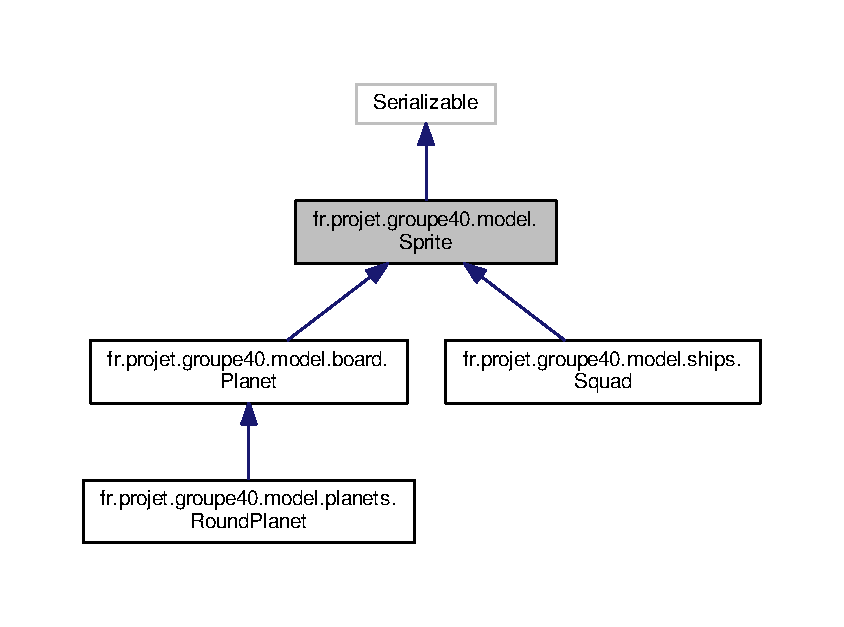
\includegraphics[width=350pt]{classfr_1_1projet_1_1groupe40_1_1model_1_1_sprite__inherit__graph}
\end{center}
\end{figure}


Collaboration diagram for fr.\+projet.\+groupe40.\+model.\+Sprite\+:\nopagebreak
\begin{figure}[H]
\begin{center}
\leavevmode
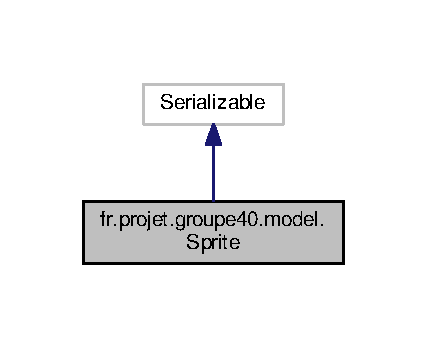
\includegraphics[width=205pt]{classfr_1_1projet_1_1groupe40_1_1model_1_1_sprite__coll__graph}
\end{center}
\end{figure}
\subsection*{Public Member Functions}
\begin{DoxyCompactItemize}
\item 
\hyperlink{classfr_1_1projet_1_1groupe40_1_1model_1_1_sprite_a043ed3640e90657015dc454876720100}{Sprite} (String path, \hyperlink{classfr_1_1projet_1_1groupe40_1_1client_1_1_user}{User} ruler, boolean is\+Planet)
\item 
void \hyperlink{classfr_1_1projet_1_1groupe40_1_1model_1_1_sprite_a8a3d06ac02e46e0348484037b5a2fbc6}{update\+Image} ()
\item 
void \hyperlink{classfr_1_1projet_1_1groupe40_1_1model_1_1_sprite_a4515fd9dbb0b4cd244a634d5c3a992a8}{set\+Position} (int x, int y)
\item 
double \hyperlink{classfr_1_1projet_1_1groupe40_1_1model_1_1_sprite_ab0288610b737af0f2419dd47001d11af}{distance} (double x, double y)
\item 
double \hyperlink{classfr_1_1projet_1_1groupe40_1_1model_1_1_sprite_a9352edb5b8b5b143fae4362e28e4a421}{distance} (double x1, double y1, double x2, double y2)
\item 
double \hyperlink{classfr_1_1projet_1_1groupe40_1_1model_1_1_sprite_adc22b47a658c0520707fb5114d2aa91e}{distance} (\hyperlink{classfr_1_1projet_1_1groupe40_1_1model_1_1_sprite}{Sprite} p)
\item 
void \hyperlink{classfr_1_1projet_1_1groupe40_1_1model_1_1_sprite_a126d99f3cbffe3706cec9faa2939e1a2}{validate\+Position} ()
\item 
boolean \hyperlink{classfr_1_1projet_1_1groupe40_1_1model_1_1_sprite_a9ceeb5eaf5ef05f293d4a1003bad9239}{intersect\+Circle} (double x\+\_\+left, double y\+\_\+top, double x\+\_\+right, double y\+\_\+bottom)
\item 
boolean \hyperlink{classfr_1_1projet_1_1groupe40_1_1model_1_1_sprite_a57c9dbd46161d5b6811e86a7c9307a36}{intersect\+Circle} (\hyperlink{classfr_1_1projet_1_1groupe40_1_1model_1_1_sprite}{Sprite} p)
\item 
boolean \hyperlink{classfr_1_1projet_1_1groupe40_1_1model_1_1_sprite_a03548b31b8fcd9b96713cbfa751ba8c5}{is\+Inside} (double x, double y, double width, double height)
\item 
boolean \hyperlink{classfr_1_1projet_1_1groupe40_1_1model_1_1_sprite_a72a8e0699c8d320b462f1d2ab185484d}{is\+Inside} (\hyperlink{classfr_1_1projet_1_1groupe40_1_1model_1_1_sprite}{Sprite} s)
\item 
void \hyperlink{classfr_1_1projet_1_1groupe40_1_1model_1_1_sprite_a9e5a351531357c8f3d7db969928492ff}{set\+Position} (double x, double y)
\item 
void \hyperlink{classfr_1_1projet_1_1groupe40_1_1model_1_1_sprite_a493d99ca3af3f1aadaafde3b49d5f76d}{set\+Speed} (double x\+Speed, double y\+Speed)
\item 
void \hyperlink{classfr_1_1projet_1_1groupe40_1_1model_1_1_sprite_a7b8ad140aa45dd17cd1158ed0bb17b41}{change\+Speed} (Key\+Code code)
\item 
void \hyperlink{classfr_1_1projet_1_1groupe40_1_1model_1_1_sprite_ac176a01b5cd31b44625b986ac6465dc4}{update\+Position} ()
\item 
void \hyperlink{classfr_1_1projet_1_1groupe40_1_1model_1_1_sprite_a49192f4485bd8773e30f8f6001da846c}{render} (Graphics\+Context gc)
\item 
boolean \hyperlink{classfr_1_1projet_1_1groupe40_1_1model_1_1_sprite_ac7b36b21ecd726d53df5b55c176d14c0}{intersects} (\hyperlink{classfr_1_1projet_1_1groupe40_1_1model_1_1_sprite}{Sprite} s)
\item 
boolean \hyperlink{classfr_1_1projet_1_1groupe40_1_1model_1_1_sprite_a8388dcfa156e3311768dc8cdee554989}{intersects} (double x2, double y2, double width, double height)
\item 
double \hyperlink{classfr_1_1projet_1_1groupe40_1_1model_1_1_sprite_ac9816a7404c674b2cb1d0fa2d1d57c16}{width} ()
\item 
double \hyperlink{classfr_1_1projet_1_1groupe40_1_1model_1_1_sprite_afc96a634b1c8e707fc0270d1f2bbdaf7}{height} ()
\item 
String \hyperlink{classfr_1_1projet_1_1groupe40_1_1model_1_1_sprite_aefa1e974157818c675f3a2a09c2a2c0c}{to\+String} ()
\item 
\hyperlink{classfr_1_1projet_1_1groupe40_1_1client_1_1_user}{User} \hyperlink{classfr_1_1projet_1_1groupe40_1_1model_1_1_sprite_adb3cc8fe7587257ec1ba0d1b11aab358}{get\+Ruler} ()
\item 
void \hyperlink{classfr_1_1projet_1_1groupe40_1_1model_1_1_sprite_aa1e2d8bbd9276ff283ffe17236fe0424}{set\+Ruler} (\hyperlink{classfr_1_1projet_1_1groupe40_1_1client_1_1_user}{User} ruler)
\item 
Image \hyperlink{classfr_1_1projet_1_1groupe40_1_1model_1_1_sprite_accf8ab35b3fe0645d7c70aa47d6ad599}{get\+Image} ()
\item 
void \hyperlink{classfr_1_1projet_1_1groupe40_1_1model_1_1_sprite_a63ee7ba27752eca98bdc4811f5c0cb29}{set\+Image} (Image image)
\item 
double \hyperlink{classfr_1_1projet_1_1groupe40_1_1model_1_1_sprite_af7f38694af58b4066533c219d49d73ea}{getX} ()
\item 
void \hyperlink{classfr_1_1projet_1_1groupe40_1_1model_1_1_sprite_af0855c92d27754fcce4503011d4edf87}{setX} (double x)
\item 
double \hyperlink{classfr_1_1projet_1_1groupe40_1_1model_1_1_sprite_a18cb2df6b166f5bb89d32235db905d30}{getY} ()
\item 
void \hyperlink{classfr_1_1projet_1_1groupe40_1_1model_1_1_sprite_aa13dfac12e80175bce81f00d60ade84d}{setY} (double y)
\item 
double \hyperlink{classfr_1_1projet_1_1groupe40_1_1model_1_1_sprite_ac2c84f9ca07ca08e3fa382df1d530483}{getx\+Speed} ()
\item 
void \hyperlink{classfr_1_1projet_1_1groupe40_1_1model_1_1_sprite_a4666a43d078d094ba67cf0e776792f7f}{setx\+Speed} (double x\+Speed)
\item 
double \hyperlink{classfr_1_1projet_1_1groupe40_1_1model_1_1_sprite_a802670e3f445d427794f7c326947edc5}{gety\+Speed} ()
\item 
void \hyperlink{classfr_1_1projet_1_1groupe40_1_1model_1_1_sprite_a8bc4c43d662b4754038f1e2483ee733b}{sety\+Speed} (double y\+Speed)
\item 
void \hyperlink{classfr_1_1projet_1_1groupe40_1_1model_1_1_sprite_ab0d054cf838a6266fca1cc07c75aaf10}{set\+Width} (double width)
\item 
void \hyperlink{classfr_1_1projet_1_1groupe40_1_1model_1_1_sprite_a77b1a9a06d941378fdfc12873da17362}{set\+Height} (double height)
\item 
String \hyperlink{classfr_1_1projet_1_1groupe40_1_1model_1_1_sprite_a1774e558697c186bd807a162ac6e525f}{get\+Img\+\_\+path} ()
\item 
void \hyperlink{classfr_1_1projet_1_1groupe40_1_1model_1_1_sprite_a8c961c15aac6e6586568c654672f6529}{set\+Img\+\_\+path} (String img\+\_\+path)
\item 
double \hyperlink{classfr_1_1projet_1_1groupe40_1_1model_1_1_sprite_a0e742e113e2ebdfa7a8b3e2d03f32816}{get\+MaxY} ()
\item 
void \hyperlink{classfr_1_1projet_1_1groupe40_1_1model_1_1_sprite_a7ed0ebd26e50a78437b47a629dc5ed97}{set\+MaxY} (double maxY)
\item 
double \hyperlink{classfr_1_1projet_1_1groupe40_1_1model_1_1_sprite_ab7532fa08a3bec8f0fc93d3b5ce53ca7}{get\+MaxX} ()
\item 
void \hyperlink{classfr_1_1projet_1_1groupe40_1_1model_1_1_sprite_a00b465c36deae2b35c582d71d9ee7836}{set\+MaxX} (double maxX)
\end{DoxyCompactItemize}


\subsection{Constructor \& Destructor Documentation}
\mbox{\Hypertarget{classfr_1_1projet_1_1groupe40_1_1model_1_1_sprite_a043ed3640e90657015dc454876720100}\label{classfr_1_1projet_1_1groupe40_1_1model_1_1_sprite_a043ed3640e90657015dc454876720100}} 
\index{fr\+::projet\+::groupe40\+::model\+::\+Sprite@{fr\+::projet\+::groupe40\+::model\+::\+Sprite}!Sprite@{Sprite}}
\index{Sprite@{Sprite}!fr\+::projet\+::groupe40\+::model\+::\+Sprite@{fr\+::projet\+::groupe40\+::model\+::\+Sprite}}
\subsubsection{\texorpdfstring{Sprite()}{Sprite()}}
{\footnotesize\ttfamily fr.\+projet.\+groupe40.\+model.\+Sprite.\+Sprite (\begin{DoxyParamCaption}\item[{String}]{path,  }\item[{\hyperlink{classfr_1_1projet_1_1groupe40_1_1client_1_1_user}{User}}]{ruler,  }\item[{boolean}]{is\+Planet }\end{DoxyParamCaption})}



\subsection{Member Function Documentation}
\mbox{\Hypertarget{classfr_1_1projet_1_1groupe40_1_1model_1_1_sprite_a7b8ad140aa45dd17cd1158ed0bb17b41}\label{classfr_1_1projet_1_1groupe40_1_1model_1_1_sprite_a7b8ad140aa45dd17cd1158ed0bb17b41}} 
\index{fr\+::projet\+::groupe40\+::model\+::\+Sprite@{fr\+::projet\+::groupe40\+::model\+::\+Sprite}!change\+Speed@{change\+Speed}}
\index{change\+Speed@{change\+Speed}!fr\+::projet\+::groupe40\+::model\+::\+Sprite@{fr\+::projet\+::groupe40\+::model\+::\+Sprite}}
\subsubsection{\texorpdfstring{change\+Speed()}{changeSpeed()}}
{\footnotesize\ttfamily void fr.\+projet.\+groupe40.\+model.\+Sprite.\+change\+Speed (\begin{DoxyParamCaption}\item[{Key\+Code}]{code }\end{DoxyParamCaption})}

\mbox{\Hypertarget{classfr_1_1projet_1_1groupe40_1_1model_1_1_sprite_ab0288610b737af0f2419dd47001d11af}\label{classfr_1_1projet_1_1groupe40_1_1model_1_1_sprite_ab0288610b737af0f2419dd47001d11af}} 
\index{fr\+::projet\+::groupe40\+::model\+::\+Sprite@{fr\+::projet\+::groupe40\+::model\+::\+Sprite}!distance@{distance}}
\index{distance@{distance}!fr\+::projet\+::groupe40\+::model\+::\+Sprite@{fr\+::projet\+::groupe40\+::model\+::\+Sprite}}
\subsubsection{\texorpdfstring{distance()}{distance()}\hspace{0.1cm}{\footnotesize\ttfamily [1/3]}}
{\footnotesize\ttfamily double fr.\+projet.\+groupe40.\+model.\+Sprite.\+distance (\begin{DoxyParamCaption}\item[{double}]{x,  }\item[{double}]{y }\end{DoxyParamCaption})}

\mbox{\Hypertarget{classfr_1_1projet_1_1groupe40_1_1model_1_1_sprite_a9352edb5b8b5b143fae4362e28e4a421}\label{classfr_1_1projet_1_1groupe40_1_1model_1_1_sprite_a9352edb5b8b5b143fae4362e28e4a421}} 
\index{fr\+::projet\+::groupe40\+::model\+::\+Sprite@{fr\+::projet\+::groupe40\+::model\+::\+Sprite}!distance@{distance}}
\index{distance@{distance}!fr\+::projet\+::groupe40\+::model\+::\+Sprite@{fr\+::projet\+::groupe40\+::model\+::\+Sprite}}
\subsubsection{\texorpdfstring{distance()}{distance()}\hspace{0.1cm}{\footnotesize\ttfamily [2/3]}}
{\footnotesize\ttfamily double fr.\+projet.\+groupe40.\+model.\+Sprite.\+distance (\begin{DoxyParamCaption}\item[{double}]{x1,  }\item[{double}]{y1,  }\item[{double}]{x2,  }\item[{double}]{y2 }\end{DoxyParamCaption})}

\mbox{\Hypertarget{classfr_1_1projet_1_1groupe40_1_1model_1_1_sprite_adc22b47a658c0520707fb5114d2aa91e}\label{classfr_1_1projet_1_1groupe40_1_1model_1_1_sprite_adc22b47a658c0520707fb5114d2aa91e}} 
\index{fr\+::projet\+::groupe40\+::model\+::\+Sprite@{fr\+::projet\+::groupe40\+::model\+::\+Sprite}!distance@{distance}}
\index{distance@{distance}!fr\+::projet\+::groupe40\+::model\+::\+Sprite@{fr\+::projet\+::groupe40\+::model\+::\+Sprite}}
\subsubsection{\texorpdfstring{distance()}{distance()}\hspace{0.1cm}{\footnotesize\ttfamily [3/3]}}
{\footnotesize\ttfamily double fr.\+projet.\+groupe40.\+model.\+Sprite.\+distance (\begin{DoxyParamCaption}\item[{\hyperlink{classfr_1_1projet_1_1groupe40_1_1model_1_1_sprite}{Sprite}}]{p }\end{DoxyParamCaption})}

\mbox{\Hypertarget{classfr_1_1projet_1_1groupe40_1_1model_1_1_sprite_accf8ab35b3fe0645d7c70aa47d6ad599}\label{classfr_1_1projet_1_1groupe40_1_1model_1_1_sprite_accf8ab35b3fe0645d7c70aa47d6ad599}} 
\index{fr\+::projet\+::groupe40\+::model\+::\+Sprite@{fr\+::projet\+::groupe40\+::model\+::\+Sprite}!get\+Image@{get\+Image}}
\index{get\+Image@{get\+Image}!fr\+::projet\+::groupe40\+::model\+::\+Sprite@{fr\+::projet\+::groupe40\+::model\+::\+Sprite}}
\subsubsection{\texorpdfstring{get\+Image()}{getImage()}}
{\footnotesize\ttfamily Image fr.\+projet.\+groupe40.\+model.\+Sprite.\+get\+Image (\begin{DoxyParamCaption}{ }\end{DoxyParamCaption})}

\mbox{\Hypertarget{classfr_1_1projet_1_1groupe40_1_1model_1_1_sprite_a1774e558697c186bd807a162ac6e525f}\label{classfr_1_1projet_1_1groupe40_1_1model_1_1_sprite_a1774e558697c186bd807a162ac6e525f}} 
\index{fr\+::projet\+::groupe40\+::model\+::\+Sprite@{fr\+::projet\+::groupe40\+::model\+::\+Sprite}!get\+Img\+\_\+path@{get\+Img\+\_\+path}}
\index{get\+Img\+\_\+path@{get\+Img\+\_\+path}!fr\+::projet\+::groupe40\+::model\+::\+Sprite@{fr\+::projet\+::groupe40\+::model\+::\+Sprite}}
\subsubsection{\texorpdfstring{get\+Img\+\_\+path()}{getImg\_path()}}
{\footnotesize\ttfamily String fr.\+projet.\+groupe40.\+model.\+Sprite.\+get\+Img\+\_\+path (\begin{DoxyParamCaption}{ }\end{DoxyParamCaption})}

\begin{DoxyReturn}{Returns}
the img\+\_\+path 
\end{DoxyReturn}
\mbox{\Hypertarget{classfr_1_1projet_1_1groupe40_1_1model_1_1_sprite_ab7532fa08a3bec8f0fc93d3b5ce53ca7}\label{classfr_1_1projet_1_1groupe40_1_1model_1_1_sprite_ab7532fa08a3bec8f0fc93d3b5ce53ca7}} 
\index{fr\+::projet\+::groupe40\+::model\+::\+Sprite@{fr\+::projet\+::groupe40\+::model\+::\+Sprite}!get\+MaxX@{get\+MaxX}}
\index{get\+MaxX@{get\+MaxX}!fr\+::projet\+::groupe40\+::model\+::\+Sprite@{fr\+::projet\+::groupe40\+::model\+::\+Sprite}}
\subsubsection{\texorpdfstring{get\+Max\+X()}{getMaxX()}}
{\footnotesize\ttfamily double fr.\+projet.\+groupe40.\+model.\+Sprite.\+get\+MaxX (\begin{DoxyParamCaption}{ }\end{DoxyParamCaption})}

\mbox{\Hypertarget{classfr_1_1projet_1_1groupe40_1_1model_1_1_sprite_a0e742e113e2ebdfa7a8b3e2d03f32816}\label{classfr_1_1projet_1_1groupe40_1_1model_1_1_sprite_a0e742e113e2ebdfa7a8b3e2d03f32816}} 
\index{fr\+::projet\+::groupe40\+::model\+::\+Sprite@{fr\+::projet\+::groupe40\+::model\+::\+Sprite}!get\+MaxY@{get\+MaxY}}
\index{get\+MaxY@{get\+MaxY}!fr\+::projet\+::groupe40\+::model\+::\+Sprite@{fr\+::projet\+::groupe40\+::model\+::\+Sprite}}
\subsubsection{\texorpdfstring{get\+Max\+Y()}{getMaxY()}}
{\footnotesize\ttfamily double fr.\+projet.\+groupe40.\+model.\+Sprite.\+get\+MaxY (\begin{DoxyParamCaption}{ }\end{DoxyParamCaption})}

\mbox{\Hypertarget{classfr_1_1projet_1_1groupe40_1_1model_1_1_sprite_adb3cc8fe7587257ec1ba0d1b11aab358}\label{classfr_1_1projet_1_1groupe40_1_1model_1_1_sprite_adb3cc8fe7587257ec1ba0d1b11aab358}} 
\index{fr\+::projet\+::groupe40\+::model\+::\+Sprite@{fr\+::projet\+::groupe40\+::model\+::\+Sprite}!get\+Ruler@{get\+Ruler}}
\index{get\+Ruler@{get\+Ruler}!fr\+::projet\+::groupe40\+::model\+::\+Sprite@{fr\+::projet\+::groupe40\+::model\+::\+Sprite}}
\subsubsection{\texorpdfstring{get\+Ruler()}{getRuler()}}
{\footnotesize\ttfamily \hyperlink{classfr_1_1projet_1_1groupe40_1_1client_1_1_user}{User} fr.\+projet.\+groupe40.\+model.\+Sprite.\+get\+Ruler (\begin{DoxyParamCaption}{ }\end{DoxyParamCaption})}

\mbox{\Hypertarget{classfr_1_1projet_1_1groupe40_1_1model_1_1_sprite_af7f38694af58b4066533c219d49d73ea}\label{classfr_1_1projet_1_1groupe40_1_1model_1_1_sprite_af7f38694af58b4066533c219d49d73ea}} 
\index{fr\+::projet\+::groupe40\+::model\+::\+Sprite@{fr\+::projet\+::groupe40\+::model\+::\+Sprite}!getX@{getX}}
\index{getX@{getX}!fr\+::projet\+::groupe40\+::model\+::\+Sprite@{fr\+::projet\+::groupe40\+::model\+::\+Sprite}}
\subsubsection{\texorpdfstring{get\+X()}{getX()}}
{\footnotesize\ttfamily double fr.\+projet.\+groupe40.\+model.\+Sprite.\+getX (\begin{DoxyParamCaption}{ }\end{DoxyParamCaption})}

\mbox{\Hypertarget{classfr_1_1projet_1_1groupe40_1_1model_1_1_sprite_ac2c84f9ca07ca08e3fa382df1d530483}\label{classfr_1_1projet_1_1groupe40_1_1model_1_1_sprite_ac2c84f9ca07ca08e3fa382df1d530483}} 
\index{fr\+::projet\+::groupe40\+::model\+::\+Sprite@{fr\+::projet\+::groupe40\+::model\+::\+Sprite}!getx\+Speed@{getx\+Speed}}
\index{getx\+Speed@{getx\+Speed}!fr\+::projet\+::groupe40\+::model\+::\+Sprite@{fr\+::projet\+::groupe40\+::model\+::\+Sprite}}
\subsubsection{\texorpdfstring{getx\+Speed()}{getxSpeed()}}
{\footnotesize\ttfamily double fr.\+projet.\+groupe40.\+model.\+Sprite.\+getx\+Speed (\begin{DoxyParamCaption}{ }\end{DoxyParamCaption})}

\mbox{\Hypertarget{classfr_1_1projet_1_1groupe40_1_1model_1_1_sprite_a18cb2df6b166f5bb89d32235db905d30}\label{classfr_1_1projet_1_1groupe40_1_1model_1_1_sprite_a18cb2df6b166f5bb89d32235db905d30}} 
\index{fr\+::projet\+::groupe40\+::model\+::\+Sprite@{fr\+::projet\+::groupe40\+::model\+::\+Sprite}!getY@{getY}}
\index{getY@{getY}!fr\+::projet\+::groupe40\+::model\+::\+Sprite@{fr\+::projet\+::groupe40\+::model\+::\+Sprite}}
\subsubsection{\texorpdfstring{get\+Y()}{getY()}}
{\footnotesize\ttfamily double fr.\+projet.\+groupe40.\+model.\+Sprite.\+getY (\begin{DoxyParamCaption}{ }\end{DoxyParamCaption})}

\mbox{\Hypertarget{classfr_1_1projet_1_1groupe40_1_1model_1_1_sprite_a802670e3f445d427794f7c326947edc5}\label{classfr_1_1projet_1_1groupe40_1_1model_1_1_sprite_a802670e3f445d427794f7c326947edc5}} 
\index{fr\+::projet\+::groupe40\+::model\+::\+Sprite@{fr\+::projet\+::groupe40\+::model\+::\+Sprite}!gety\+Speed@{gety\+Speed}}
\index{gety\+Speed@{gety\+Speed}!fr\+::projet\+::groupe40\+::model\+::\+Sprite@{fr\+::projet\+::groupe40\+::model\+::\+Sprite}}
\subsubsection{\texorpdfstring{gety\+Speed()}{getySpeed()}}
{\footnotesize\ttfamily double fr.\+projet.\+groupe40.\+model.\+Sprite.\+gety\+Speed (\begin{DoxyParamCaption}{ }\end{DoxyParamCaption})}

\mbox{\Hypertarget{classfr_1_1projet_1_1groupe40_1_1model_1_1_sprite_afc96a634b1c8e707fc0270d1f2bbdaf7}\label{classfr_1_1projet_1_1groupe40_1_1model_1_1_sprite_afc96a634b1c8e707fc0270d1f2bbdaf7}} 
\index{fr\+::projet\+::groupe40\+::model\+::\+Sprite@{fr\+::projet\+::groupe40\+::model\+::\+Sprite}!height@{height}}
\index{height@{height}!fr\+::projet\+::groupe40\+::model\+::\+Sprite@{fr\+::projet\+::groupe40\+::model\+::\+Sprite}}
\subsubsection{\texorpdfstring{height()}{height()}}
{\footnotesize\ttfamily double fr.\+projet.\+groupe40.\+model.\+Sprite.\+height (\begin{DoxyParamCaption}{ }\end{DoxyParamCaption})}

\mbox{\Hypertarget{classfr_1_1projet_1_1groupe40_1_1model_1_1_sprite_a9ceeb5eaf5ef05f293d4a1003bad9239}\label{classfr_1_1projet_1_1groupe40_1_1model_1_1_sprite_a9ceeb5eaf5ef05f293d4a1003bad9239}} 
\index{fr\+::projet\+::groupe40\+::model\+::\+Sprite@{fr\+::projet\+::groupe40\+::model\+::\+Sprite}!intersect\+Circle@{intersect\+Circle}}
\index{intersect\+Circle@{intersect\+Circle}!fr\+::projet\+::groupe40\+::model\+::\+Sprite@{fr\+::projet\+::groupe40\+::model\+::\+Sprite}}
\subsubsection{\texorpdfstring{intersect\+Circle()}{intersectCircle()}\hspace{0.1cm}{\footnotesize\ttfamily [1/2]}}
{\footnotesize\ttfamily boolean fr.\+projet.\+groupe40.\+model.\+Sprite.\+intersect\+Circle (\begin{DoxyParamCaption}\item[{double}]{x\+\_\+left,  }\item[{double}]{y\+\_\+top,  }\item[{double}]{x\+\_\+right,  }\item[{double}]{y\+\_\+bottom }\end{DoxyParamCaption})}

\mbox{\Hypertarget{classfr_1_1projet_1_1groupe40_1_1model_1_1_sprite_a57c9dbd46161d5b6811e86a7c9307a36}\label{classfr_1_1projet_1_1groupe40_1_1model_1_1_sprite_a57c9dbd46161d5b6811e86a7c9307a36}} 
\index{fr\+::projet\+::groupe40\+::model\+::\+Sprite@{fr\+::projet\+::groupe40\+::model\+::\+Sprite}!intersect\+Circle@{intersect\+Circle}}
\index{intersect\+Circle@{intersect\+Circle}!fr\+::projet\+::groupe40\+::model\+::\+Sprite@{fr\+::projet\+::groupe40\+::model\+::\+Sprite}}
\subsubsection{\texorpdfstring{intersect\+Circle()}{intersectCircle()}\hspace{0.1cm}{\footnotesize\ttfamily [2/2]}}
{\footnotesize\ttfamily boolean fr.\+projet.\+groupe40.\+model.\+Sprite.\+intersect\+Circle (\begin{DoxyParamCaption}\item[{\hyperlink{classfr_1_1projet_1_1groupe40_1_1model_1_1_sprite}{Sprite}}]{p }\end{DoxyParamCaption})}

\mbox{\Hypertarget{classfr_1_1projet_1_1groupe40_1_1model_1_1_sprite_ac7b36b21ecd726d53df5b55c176d14c0}\label{classfr_1_1projet_1_1groupe40_1_1model_1_1_sprite_ac7b36b21ecd726d53df5b55c176d14c0}} 
\index{fr\+::projet\+::groupe40\+::model\+::\+Sprite@{fr\+::projet\+::groupe40\+::model\+::\+Sprite}!intersects@{intersects}}
\index{intersects@{intersects}!fr\+::projet\+::groupe40\+::model\+::\+Sprite@{fr\+::projet\+::groupe40\+::model\+::\+Sprite}}
\subsubsection{\texorpdfstring{intersects()}{intersects()}\hspace{0.1cm}{\footnotesize\ttfamily [1/2]}}
{\footnotesize\ttfamily boolean fr.\+projet.\+groupe40.\+model.\+Sprite.\+intersects (\begin{DoxyParamCaption}\item[{\hyperlink{classfr_1_1projet_1_1groupe40_1_1model_1_1_sprite}{Sprite}}]{s }\end{DoxyParamCaption})}

\mbox{\Hypertarget{classfr_1_1projet_1_1groupe40_1_1model_1_1_sprite_a8388dcfa156e3311768dc8cdee554989}\label{classfr_1_1projet_1_1groupe40_1_1model_1_1_sprite_a8388dcfa156e3311768dc8cdee554989}} 
\index{fr\+::projet\+::groupe40\+::model\+::\+Sprite@{fr\+::projet\+::groupe40\+::model\+::\+Sprite}!intersects@{intersects}}
\index{intersects@{intersects}!fr\+::projet\+::groupe40\+::model\+::\+Sprite@{fr\+::projet\+::groupe40\+::model\+::\+Sprite}}
\subsubsection{\texorpdfstring{intersects()}{intersects()}\hspace{0.1cm}{\footnotesize\ttfamily [2/2]}}
{\footnotesize\ttfamily boolean fr.\+projet.\+groupe40.\+model.\+Sprite.\+intersects (\begin{DoxyParamCaption}\item[{double}]{x2,  }\item[{double}]{y2,  }\item[{double}]{width,  }\item[{double}]{height }\end{DoxyParamCaption})}

\mbox{\Hypertarget{classfr_1_1projet_1_1groupe40_1_1model_1_1_sprite_a03548b31b8fcd9b96713cbfa751ba8c5}\label{classfr_1_1projet_1_1groupe40_1_1model_1_1_sprite_a03548b31b8fcd9b96713cbfa751ba8c5}} 
\index{fr\+::projet\+::groupe40\+::model\+::\+Sprite@{fr\+::projet\+::groupe40\+::model\+::\+Sprite}!is\+Inside@{is\+Inside}}
\index{is\+Inside@{is\+Inside}!fr\+::projet\+::groupe40\+::model\+::\+Sprite@{fr\+::projet\+::groupe40\+::model\+::\+Sprite}}
\subsubsection{\texorpdfstring{is\+Inside()}{isInside()}\hspace{0.1cm}{\footnotesize\ttfamily [1/2]}}
{\footnotesize\ttfamily boolean fr.\+projet.\+groupe40.\+model.\+Sprite.\+is\+Inside (\begin{DoxyParamCaption}\item[{double}]{x,  }\item[{double}]{y,  }\item[{double}]{width,  }\item[{double}]{height }\end{DoxyParamCaption})}

\mbox{\Hypertarget{classfr_1_1projet_1_1groupe40_1_1model_1_1_sprite_a72a8e0699c8d320b462f1d2ab185484d}\label{classfr_1_1projet_1_1groupe40_1_1model_1_1_sprite_a72a8e0699c8d320b462f1d2ab185484d}} 
\index{fr\+::projet\+::groupe40\+::model\+::\+Sprite@{fr\+::projet\+::groupe40\+::model\+::\+Sprite}!is\+Inside@{is\+Inside}}
\index{is\+Inside@{is\+Inside}!fr\+::projet\+::groupe40\+::model\+::\+Sprite@{fr\+::projet\+::groupe40\+::model\+::\+Sprite}}
\subsubsection{\texorpdfstring{is\+Inside()}{isInside()}\hspace{0.1cm}{\footnotesize\ttfamily [2/2]}}
{\footnotesize\ttfamily boolean fr.\+projet.\+groupe40.\+model.\+Sprite.\+is\+Inside (\begin{DoxyParamCaption}\item[{\hyperlink{classfr_1_1projet_1_1groupe40_1_1model_1_1_sprite}{Sprite}}]{s }\end{DoxyParamCaption})}

\mbox{\Hypertarget{classfr_1_1projet_1_1groupe40_1_1model_1_1_sprite_a49192f4485bd8773e30f8f6001da846c}\label{classfr_1_1projet_1_1groupe40_1_1model_1_1_sprite_a49192f4485bd8773e30f8f6001da846c}} 
\index{fr\+::projet\+::groupe40\+::model\+::\+Sprite@{fr\+::projet\+::groupe40\+::model\+::\+Sprite}!render@{render}}
\index{render@{render}!fr\+::projet\+::groupe40\+::model\+::\+Sprite@{fr\+::projet\+::groupe40\+::model\+::\+Sprite}}
\subsubsection{\texorpdfstring{render()}{render()}}
{\footnotesize\ttfamily void fr.\+projet.\+groupe40.\+model.\+Sprite.\+render (\begin{DoxyParamCaption}\item[{Graphics\+Context}]{gc }\end{DoxyParamCaption})}

\mbox{\Hypertarget{classfr_1_1projet_1_1groupe40_1_1model_1_1_sprite_a77b1a9a06d941378fdfc12873da17362}\label{classfr_1_1projet_1_1groupe40_1_1model_1_1_sprite_a77b1a9a06d941378fdfc12873da17362}} 
\index{fr\+::projet\+::groupe40\+::model\+::\+Sprite@{fr\+::projet\+::groupe40\+::model\+::\+Sprite}!set\+Height@{set\+Height}}
\index{set\+Height@{set\+Height}!fr\+::projet\+::groupe40\+::model\+::\+Sprite@{fr\+::projet\+::groupe40\+::model\+::\+Sprite}}
\subsubsection{\texorpdfstring{set\+Height()}{setHeight()}}
{\footnotesize\ttfamily void fr.\+projet.\+groupe40.\+model.\+Sprite.\+set\+Height (\begin{DoxyParamCaption}\item[{double}]{height }\end{DoxyParamCaption})}


\begin{DoxyParams}{Parameters}
{\em height} & the height to set \\
\hline
\end{DoxyParams}
\mbox{\Hypertarget{classfr_1_1projet_1_1groupe40_1_1model_1_1_sprite_a63ee7ba27752eca98bdc4811f5c0cb29}\label{classfr_1_1projet_1_1groupe40_1_1model_1_1_sprite_a63ee7ba27752eca98bdc4811f5c0cb29}} 
\index{fr\+::projet\+::groupe40\+::model\+::\+Sprite@{fr\+::projet\+::groupe40\+::model\+::\+Sprite}!set\+Image@{set\+Image}}
\index{set\+Image@{set\+Image}!fr\+::projet\+::groupe40\+::model\+::\+Sprite@{fr\+::projet\+::groupe40\+::model\+::\+Sprite}}
\subsubsection{\texorpdfstring{set\+Image()}{setImage()}}
{\footnotesize\ttfamily void fr.\+projet.\+groupe40.\+model.\+Sprite.\+set\+Image (\begin{DoxyParamCaption}\item[{Image}]{image }\end{DoxyParamCaption})}

\mbox{\Hypertarget{classfr_1_1projet_1_1groupe40_1_1model_1_1_sprite_a8c961c15aac6e6586568c654672f6529}\label{classfr_1_1projet_1_1groupe40_1_1model_1_1_sprite_a8c961c15aac6e6586568c654672f6529}} 
\index{fr\+::projet\+::groupe40\+::model\+::\+Sprite@{fr\+::projet\+::groupe40\+::model\+::\+Sprite}!set\+Img\+\_\+path@{set\+Img\+\_\+path}}
\index{set\+Img\+\_\+path@{set\+Img\+\_\+path}!fr\+::projet\+::groupe40\+::model\+::\+Sprite@{fr\+::projet\+::groupe40\+::model\+::\+Sprite}}
\subsubsection{\texorpdfstring{set\+Img\+\_\+path()}{setImg\_path()}}
{\footnotesize\ttfamily void fr.\+projet.\+groupe40.\+model.\+Sprite.\+set\+Img\+\_\+path (\begin{DoxyParamCaption}\item[{String}]{img\+\_\+path }\end{DoxyParamCaption})}


\begin{DoxyParams}{Parameters}
{\em img\+\_\+path} & the img\+\_\+path to set \\
\hline
\end{DoxyParams}
\mbox{\Hypertarget{classfr_1_1projet_1_1groupe40_1_1model_1_1_sprite_a00b465c36deae2b35c582d71d9ee7836}\label{classfr_1_1projet_1_1groupe40_1_1model_1_1_sprite_a00b465c36deae2b35c582d71d9ee7836}} 
\index{fr\+::projet\+::groupe40\+::model\+::\+Sprite@{fr\+::projet\+::groupe40\+::model\+::\+Sprite}!set\+MaxX@{set\+MaxX}}
\index{set\+MaxX@{set\+MaxX}!fr\+::projet\+::groupe40\+::model\+::\+Sprite@{fr\+::projet\+::groupe40\+::model\+::\+Sprite}}
\subsubsection{\texorpdfstring{set\+Max\+X()}{setMaxX()}}
{\footnotesize\ttfamily void fr.\+projet.\+groupe40.\+model.\+Sprite.\+set\+MaxX (\begin{DoxyParamCaption}\item[{double}]{maxX }\end{DoxyParamCaption})}

\mbox{\Hypertarget{classfr_1_1projet_1_1groupe40_1_1model_1_1_sprite_a7ed0ebd26e50a78437b47a629dc5ed97}\label{classfr_1_1projet_1_1groupe40_1_1model_1_1_sprite_a7ed0ebd26e50a78437b47a629dc5ed97}} 
\index{fr\+::projet\+::groupe40\+::model\+::\+Sprite@{fr\+::projet\+::groupe40\+::model\+::\+Sprite}!set\+MaxY@{set\+MaxY}}
\index{set\+MaxY@{set\+MaxY}!fr\+::projet\+::groupe40\+::model\+::\+Sprite@{fr\+::projet\+::groupe40\+::model\+::\+Sprite}}
\subsubsection{\texorpdfstring{set\+Max\+Y()}{setMaxY()}}
{\footnotesize\ttfamily void fr.\+projet.\+groupe40.\+model.\+Sprite.\+set\+MaxY (\begin{DoxyParamCaption}\item[{double}]{maxY }\end{DoxyParamCaption})}

\mbox{\Hypertarget{classfr_1_1projet_1_1groupe40_1_1model_1_1_sprite_a4515fd9dbb0b4cd244a634d5c3a992a8}\label{classfr_1_1projet_1_1groupe40_1_1model_1_1_sprite_a4515fd9dbb0b4cd244a634d5c3a992a8}} 
\index{fr\+::projet\+::groupe40\+::model\+::\+Sprite@{fr\+::projet\+::groupe40\+::model\+::\+Sprite}!set\+Position@{set\+Position}}
\index{set\+Position@{set\+Position}!fr\+::projet\+::groupe40\+::model\+::\+Sprite@{fr\+::projet\+::groupe40\+::model\+::\+Sprite}}
\subsubsection{\texorpdfstring{set\+Position()}{setPosition()}\hspace{0.1cm}{\footnotesize\ttfamily [1/2]}}
{\footnotesize\ttfamily void fr.\+projet.\+groupe40.\+model.\+Sprite.\+set\+Position (\begin{DoxyParamCaption}\item[{int}]{x,  }\item[{int}]{y }\end{DoxyParamCaption})}

\mbox{\Hypertarget{classfr_1_1projet_1_1groupe40_1_1model_1_1_sprite_a9e5a351531357c8f3d7db969928492ff}\label{classfr_1_1projet_1_1groupe40_1_1model_1_1_sprite_a9e5a351531357c8f3d7db969928492ff}} 
\index{fr\+::projet\+::groupe40\+::model\+::\+Sprite@{fr\+::projet\+::groupe40\+::model\+::\+Sprite}!set\+Position@{set\+Position}}
\index{set\+Position@{set\+Position}!fr\+::projet\+::groupe40\+::model\+::\+Sprite@{fr\+::projet\+::groupe40\+::model\+::\+Sprite}}
\subsubsection{\texorpdfstring{set\+Position()}{setPosition()}\hspace{0.1cm}{\footnotesize\ttfamily [2/2]}}
{\footnotesize\ttfamily void fr.\+projet.\+groupe40.\+model.\+Sprite.\+set\+Position (\begin{DoxyParamCaption}\item[{double}]{x,  }\item[{double}]{y }\end{DoxyParamCaption})}

\mbox{\Hypertarget{classfr_1_1projet_1_1groupe40_1_1model_1_1_sprite_aa1e2d8bbd9276ff283ffe17236fe0424}\label{classfr_1_1projet_1_1groupe40_1_1model_1_1_sprite_aa1e2d8bbd9276ff283ffe17236fe0424}} 
\index{fr\+::projet\+::groupe40\+::model\+::\+Sprite@{fr\+::projet\+::groupe40\+::model\+::\+Sprite}!set\+Ruler@{set\+Ruler}}
\index{set\+Ruler@{set\+Ruler}!fr\+::projet\+::groupe40\+::model\+::\+Sprite@{fr\+::projet\+::groupe40\+::model\+::\+Sprite}}
\subsubsection{\texorpdfstring{set\+Ruler()}{setRuler()}}
{\footnotesize\ttfamily void fr.\+projet.\+groupe40.\+model.\+Sprite.\+set\+Ruler (\begin{DoxyParamCaption}\item[{\hyperlink{classfr_1_1projet_1_1groupe40_1_1client_1_1_user}{User}}]{ruler }\end{DoxyParamCaption})}

\mbox{\Hypertarget{classfr_1_1projet_1_1groupe40_1_1model_1_1_sprite_a493d99ca3af3f1aadaafde3b49d5f76d}\label{classfr_1_1projet_1_1groupe40_1_1model_1_1_sprite_a493d99ca3af3f1aadaafde3b49d5f76d}} 
\index{fr\+::projet\+::groupe40\+::model\+::\+Sprite@{fr\+::projet\+::groupe40\+::model\+::\+Sprite}!set\+Speed@{set\+Speed}}
\index{set\+Speed@{set\+Speed}!fr\+::projet\+::groupe40\+::model\+::\+Sprite@{fr\+::projet\+::groupe40\+::model\+::\+Sprite}}
\subsubsection{\texorpdfstring{set\+Speed()}{setSpeed()}}
{\footnotesize\ttfamily void fr.\+projet.\+groupe40.\+model.\+Sprite.\+set\+Speed (\begin{DoxyParamCaption}\item[{double}]{x\+Speed,  }\item[{double}]{y\+Speed }\end{DoxyParamCaption})}

\mbox{\Hypertarget{classfr_1_1projet_1_1groupe40_1_1model_1_1_sprite_ab0d054cf838a6266fca1cc07c75aaf10}\label{classfr_1_1projet_1_1groupe40_1_1model_1_1_sprite_ab0d054cf838a6266fca1cc07c75aaf10}} 
\index{fr\+::projet\+::groupe40\+::model\+::\+Sprite@{fr\+::projet\+::groupe40\+::model\+::\+Sprite}!set\+Width@{set\+Width}}
\index{set\+Width@{set\+Width}!fr\+::projet\+::groupe40\+::model\+::\+Sprite@{fr\+::projet\+::groupe40\+::model\+::\+Sprite}}
\subsubsection{\texorpdfstring{set\+Width()}{setWidth()}}
{\footnotesize\ttfamily void fr.\+projet.\+groupe40.\+model.\+Sprite.\+set\+Width (\begin{DoxyParamCaption}\item[{double}]{width }\end{DoxyParamCaption})}


\begin{DoxyParams}{Parameters}
{\em width} & the width to set \\
\hline
\end{DoxyParams}
\mbox{\Hypertarget{classfr_1_1projet_1_1groupe40_1_1model_1_1_sprite_af0855c92d27754fcce4503011d4edf87}\label{classfr_1_1projet_1_1groupe40_1_1model_1_1_sprite_af0855c92d27754fcce4503011d4edf87}} 
\index{fr\+::projet\+::groupe40\+::model\+::\+Sprite@{fr\+::projet\+::groupe40\+::model\+::\+Sprite}!setX@{setX}}
\index{setX@{setX}!fr\+::projet\+::groupe40\+::model\+::\+Sprite@{fr\+::projet\+::groupe40\+::model\+::\+Sprite}}
\subsubsection{\texorpdfstring{set\+X()}{setX()}}
{\footnotesize\ttfamily void fr.\+projet.\+groupe40.\+model.\+Sprite.\+setX (\begin{DoxyParamCaption}\item[{double}]{x }\end{DoxyParamCaption})}

\mbox{\Hypertarget{classfr_1_1projet_1_1groupe40_1_1model_1_1_sprite_a4666a43d078d094ba67cf0e776792f7f}\label{classfr_1_1projet_1_1groupe40_1_1model_1_1_sprite_a4666a43d078d094ba67cf0e776792f7f}} 
\index{fr\+::projet\+::groupe40\+::model\+::\+Sprite@{fr\+::projet\+::groupe40\+::model\+::\+Sprite}!setx\+Speed@{setx\+Speed}}
\index{setx\+Speed@{setx\+Speed}!fr\+::projet\+::groupe40\+::model\+::\+Sprite@{fr\+::projet\+::groupe40\+::model\+::\+Sprite}}
\subsubsection{\texorpdfstring{setx\+Speed()}{setxSpeed()}}
{\footnotesize\ttfamily void fr.\+projet.\+groupe40.\+model.\+Sprite.\+setx\+Speed (\begin{DoxyParamCaption}\item[{double}]{x\+Speed }\end{DoxyParamCaption})}

\mbox{\Hypertarget{classfr_1_1projet_1_1groupe40_1_1model_1_1_sprite_aa13dfac12e80175bce81f00d60ade84d}\label{classfr_1_1projet_1_1groupe40_1_1model_1_1_sprite_aa13dfac12e80175bce81f00d60ade84d}} 
\index{fr\+::projet\+::groupe40\+::model\+::\+Sprite@{fr\+::projet\+::groupe40\+::model\+::\+Sprite}!setY@{setY}}
\index{setY@{setY}!fr\+::projet\+::groupe40\+::model\+::\+Sprite@{fr\+::projet\+::groupe40\+::model\+::\+Sprite}}
\subsubsection{\texorpdfstring{set\+Y()}{setY()}}
{\footnotesize\ttfamily void fr.\+projet.\+groupe40.\+model.\+Sprite.\+setY (\begin{DoxyParamCaption}\item[{double}]{y }\end{DoxyParamCaption})}

\mbox{\Hypertarget{classfr_1_1projet_1_1groupe40_1_1model_1_1_sprite_a8bc4c43d662b4754038f1e2483ee733b}\label{classfr_1_1projet_1_1groupe40_1_1model_1_1_sprite_a8bc4c43d662b4754038f1e2483ee733b}} 
\index{fr\+::projet\+::groupe40\+::model\+::\+Sprite@{fr\+::projet\+::groupe40\+::model\+::\+Sprite}!sety\+Speed@{sety\+Speed}}
\index{sety\+Speed@{sety\+Speed}!fr\+::projet\+::groupe40\+::model\+::\+Sprite@{fr\+::projet\+::groupe40\+::model\+::\+Sprite}}
\subsubsection{\texorpdfstring{sety\+Speed()}{setySpeed()}}
{\footnotesize\ttfamily void fr.\+projet.\+groupe40.\+model.\+Sprite.\+sety\+Speed (\begin{DoxyParamCaption}\item[{double}]{y\+Speed }\end{DoxyParamCaption})}

\mbox{\Hypertarget{classfr_1_1projet_1_1groupe40_1_1model_1_1_sprite_aefa1e974157818c675f3a2a09c2a2c0c}\label{classfr_1_1projet_1_1groupe40_1_1model_1_1_sprite_aefa1e974157818c675f3a2a09c2a2c0c}} 
\index{fr\+::projet\+::groupe40\+::model\+::\+Sprite@{fr\+::projet\+::groupe40\+::model\+::\+Sprite}!to\+String@{to\+String}}
\index{to\+String@{to\+String}!fr\+::projet\+::groupe40\+::model\+::\+Sprite@{fr\+::projet\+::groupe40\+::model\+::\+Sprite}}
\subsubsection{\texorpdfstring{to\+String()}{toString()}}
{\footnotesize\ttfamily String fr.\+projet.\+groupe40.\+model.\+Sprite.\+to\+String (\begin{DoxyParamCaption}{ }\end{DoxyParamCaption})}

\mbox{\Hypertarget{classfr_1_1projet_1_1groupe40_1_1model_1_1_sprite_a8a3d06ac02e46e0348484037b5a2fbc6}\label{classfr_1_1projet_1_1groupe40_1_1model_1_1_sprite_a8a3d06ac02e46e0348484037b5a2fbc6}} 
\index{fr\+::projet\+::groupe40\+::model\+::\+Sprite@{fr\+::projet\+::groupe40\+::model\+::\+Sprite}!update\+Image@{update\+Image}}
\index{update\+Image@{update\+Image}!fr\+::projet\+::groupe40\+::model\+::\+Sprite@{fr\+::projet\+::groupe40\+::model\+::\+Sprite}}
\subsubsection{\texorpdfstring{update\+Image()}{updateImage()}}
{\footnotesize\ttfamily void fr.\+projet.\+groupe40.\+model.\+Sprite.\+update\+Image (\begin{DoxyParamCaption}{ }\end{DoxyParamCaption})}

\mbox{\Hypertarget{classfr_1_1projet_1_1groupe40_1_1model_1_1_sprite_ac176a01b5cd31b44625b986ac6465dc4}\label{classfr_1_1projet_1_1groupe40_1_1model_1_1_sprite_ac176a01b5cd31b44625b986ac6465dc4}} 
\index{fr\+::projet\+::groupe40\+::model\+::\+Sprite@{fr\+::projet\+::groupe40\+::model\+::\+Sprite}!update\+Position@{update\+Position}}
\index{update\+Position@{update\+Position}!fr\+::projet\+::groupe40\+::model\+::\+Sprite@{fr\+::projet\+::groupe40\+::model\+::\+Sprite}}
\subsubsection{\texorpdfstring{update\+Position()}{updatePosition()}}
{\footnotesize\ttfamily void fr.\+projet.\+groupe40.\+model.\+Sprite.\+update\+Position (\begin{DoxyParamCaption}{ }\end{DoxyParamCaption})}

\mbox{\Hypertarget{classfr_1_1projet_1_1groupe40_1_1model_1_1_sprite_a126d99f3cbffe3706cec9faa2939e1a2}\label{classfr_1_1projet_1_1groupe40_1_1model_1_1_sprite_a126d99f3cbffe3706cec9faa2939e1a2}} 
\index{fr\+::projet\+::groupe40\+::model\+::\+Sprite@{fr\+::projet\+::groupe40\+::model\+::\+Sprite}!validate\+Position@{validate\+Position}}
\index{validate\+Position@{validate\+Position}!fr\+::projet\+::groupe40\+::model\+::\+Sprite@{fr\+::projet\+::groupe40\+::model\+::\+Sprite}}
\subsubsection{\texorpdfstring{validate\+Position()}{validatePosition()}}
{\footnotesize\ttfamily void fr.\+projet.\+groupe40.\+model.\+Sprite.\+validate\+Position (\begin{DoxyParamCaption}{ }\end{DoxyParamCaption})}

\mbox{\Hypertarget{classfr_1_1projet_1_1groupe40_1_1model_1_1_sprite_ac9816a7404c674b2cb1d0fa2d1d57c16}\label{classfr_1_1projet_1_1groupe40_1_1model_1_1_sprite_ac9816a7404c674b2cb1d0fa2d1d57c16}} 
\index{fr\+::projet\+::groupe40\+::model\+::\+Sprite@{fr\+::projet\+::groupe40\+::model\+::\+Sprite}!width@{width}}
\index{width@{width}!fr\+::projet\+::groupe40\+::model\+::\+Sprite@{fr\+::projet\+::groupe40\+::model\+::\+Sprite}}
\subsubsection{\texorpdfstring{width()}{width()}}
{\footnotesize\ttfamily double fr.\+projet.\+groupe40.\+model.\+Sprite.\+width (\begin{DoxyParamCaption}{ }\end{DoxyParamCaption})}

Conflict Area Getter \& Setter 

The documentation for this class was generated from the following file\+:\begin{DoxyCompactItemize}
\item 
src/fr/projet/groupe40/model/\hyperlink{_sprite_8java}{Sprite.\+java}\end{DoxyCompactItemize}

\hypertarget{classfr_1_1projet_1_1groupe40_1_1model_1_1ships_1_1_squad}{}\section{fr.\+projet.\+groupe40.\+model.\+ships.\+Squad Class Reference}
\label{classfr_1_1projet_1_1groupe40_1_1model_1_1ships_1_1_squad}\index{fr.\+projet.\+groupe40.\+model.\+ships.\+Squad@{fr.\+projet.\+groupe40.\+model.\+ships.\+Squad}}


Inheritance diagram for fr.\+projet.\+groupe40.\+model.\+ships.\+Squad\+:\nopagebreak
\begin{figure}[H]
\begin{center}
\leavevmode
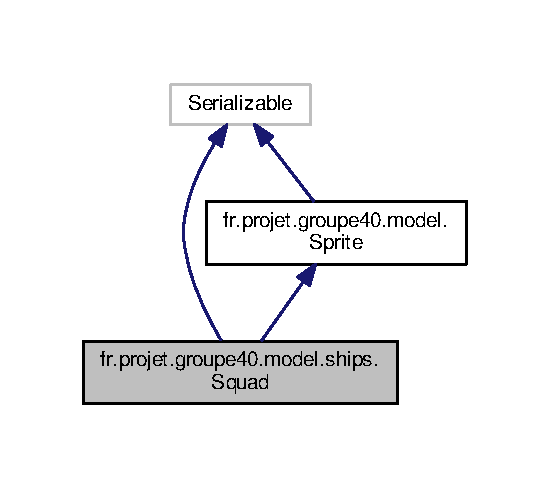
\includegraphics[width=264pt]{classfr_1_1projet_1_1groupe40_1_1model_1_1ships_1_1_squad__inherit__graph}
\end{center}
\end{figure}


Collaboration diagram for fr.\+projet.\+groupe40.\+model.\+ships.\+Squad\+:\nopagebreak
\begin{figure}[H]
\begin{center}
\leavevmode
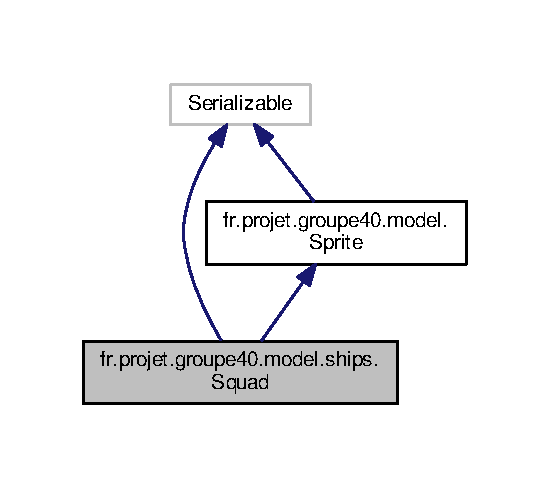
\includegraphics[width=264pt]{classfr_1_1projet_1_1groupe40_1_1model_1_1ships_1_1_squad__coll__graph}
\end{center}
\end{figure}
\subsection*{Public Member Functions}
\begin{DoxyCompactItemize}
\item 
\hyperlink{classfr_1_1projet_1_1groupe40_1_1model_1_1ships_1_1_squad_a5006326c653ad0f70f3092e7668d2c8d}{Squad} (String path, \hyperlink{classfr_1_1projet_1_1groupe40_1_1client_1_1_user}{User} user, boolean b, int nb\+\_\+of\+\_\+ships, \hyperlink{classfr_1_1projet_1_1groupe40_1_1model_1_1board_1_1_planet}{Planet} destination)
\item 
\hyperlink{classfr_1_1projet_1_1groupe40_1_1model_1_1ships_1_1_squad_a7221e4325db91f455b59652d047cddac}{Squad} (String path, \hyperlink{classfr_1_1projet_1_1groupe40_1_1client_1_1_user}{User} user, boolean b, int nb\+\_\+of\+\_\+ships, \hyperlink{classfr_1_1projet_1_1groupe40_1_1model_1_1board_1_1_planet}{Planet} destination, \hyperlink{classfr_1_1projet_1_1groupe40_1_1model_1_1ships_1_1_ship}{Ship} ships\+\_\+type)
\item 
void \hyperlink{classfr_1_1projet_1_1groupe40_1_1model_1_1ships_1_1_squad_ae7fb9263567ec5ad1c6a01845333b753}{set\+Position} (double x, double y)
\item 
void \hyperlink{classfr_1_1projet_1_1groupe40_1_1model_1_1ships_1_1_squad_aa3d39dd0446ca8939c385a7471b186a1}{remove} ()
\item 
void \hyperlink{classfr_1_1projet_1_1groupe40_1_1model_1_1ships_1_1_squad_a855ab9912a024f5a1bc680c8ecd061a3}{update\+Position} ()
\item 
int \hyperlink{classfr_1_1projet_1_1groupe40_1_1model_1_1ships_1_1_squad_adf99f4d47006c04a59fe76dae0abb8fa}{get\+Nb\+\_\+of\+\_\+ships} ()
\item 
void \hyperlink{classfr_1_1projet_1_1groupe40_1_1model_1_1ships_1_1_squad_aa106ce152e4f2e4e47cfea4ec49f0a7c}{set\+Nb\+\_\+of\+\_\+ships} (int nb\+\_\+of\+\_\+ships)
\item 
boolean \hyperlink{classfr_1_1projet_1_1groupe40_1_1model_1_1ships_1_1_squad_a8ca0c8e975e4218753d0cedf785c090d}{is\+Reached} ()
\item 
void \hyperlink{classfr_1_1projet_1_1groupe40_1_1model_1_1ships_1_1_squad_a2b19d260f6704c20adf55f8d9bbb8507}{set\+Reached} (boolean reached)
\item 
\hyperlink{classfr_1_1projet_1_1groupe40_1_1model_1_1board_1_1_planet}{Planet} \hyperlink{classfr_1_1projet_1_1groupe40_1_1model_1_1ships_1_1_squad_aa5362a9a9f99f3e9e43a4421bf78792c}{get\+Destination} ()
\item 
void \hyperlink{classfr_1_1projet_1_1groupe40_1_1model_1_1ships_1_1_squad_a04e7c22fbd42071df3c61a502f268175}{set\+Destination} (\hyperlink{classfr_1_1projet_1_1groupe40_1_1model_1_1board_1_1_planet}{Planet} destination)
\item 
String \hyperlink{classfr_1_1projet_1_1groupe40_1_1model_1_1ships_1_1_squad_a64a7b3b5df69be42303e16111d0adcdc}{to\+String} ()
\item 
\hyperlink{classfr_1_1projet_1_1groupe40_1_1model_1_1board_1_1_planet}{Planet} \hyperlink{classfr_1_1projet_1_1groupe40_1_1model_1_1ships_1_1_squad_a16980138bd442c9251eb1ede83b1b38f}{get\+Source} ()
\item 
void \hyperlink{classfr_1_1projet_1_1groupe40_1_1model_1_1ships_1_1_squad_aa670ae5e499a268d8379c3745c0d6ab7}{set\+Source} (\hyperlink{classfr_1_1projet_1_1groupe40_1_1model_1_1board_1_1_planet}{Planet} source)
\item 
\hyperlink{classfr_1_1projet_1_1groupe40_1_1model_1_1ships_1_1_ship}{Ship} \hyperlink{classfr_1_1projet_1_1groupe40_1_1model_1_1ships_1_1_squad_afb409e6b72c20f3050ebd9824237e68b}{get\+Type} ()
\item 
void \hyperlink{classfr_1_1projet_1_1groupe40_1_1model_1_1ships_1_1_squad_add7441bccd26d43a2fcea725a5d35e3a}{set\+Type} (\hyperlink{classfr_1_1projet_1_1groupe40_1_1model_1_1ships_1_1_ship}{Ship} type)
\end{DoxyCompactItemize}


\subsection{Constructor \& Destructor Documentation}
\mbox{\Hypertarget{classfr_1_1projet_1_1groupe40_1_1model_1_1ships_1_1_squad_a5006326c653ad0f70f3092e7668d2c8d}\label{classfr_1_1projet_1_1groupe40_1_1model_1_1ships_1_1_squad_a5006326c653ad0f70f3092e7668d2c8d}} 
\index{fr\+::projet\+::groupe40\+::model\+::ships\+::\+Squad@{fr\+::projet\+::groupe40\+::model\+::ships\+::\+Squad}!Squad@{Squad}}
\index{Squad@{Squad}!fr\+::projet\+::groupe40\+::model\+::ships\+::\+Squad@{fr\+::projet\+::groupe40\+::model\+::ships\+::\+Squad}}
\subsubsection{\texorpdfstring{Squad()}{Squad()}\hspace{0.1cm}{\footnotesize\ttfamily [1/2]}}
{\footnotesize\ttfamily fr.\+projet.\+groupe40.\+model.\+ships.\+Squad.\+Squad (\begin{DoxyParamCaption}\item[{String}]{path,  }\item[{\hyperlink{classfr_1_1projet_1_1groupe40_1_1client_1_1_user}{User}}]{user,  }\item[{boolean}]{b,  }\item[{int}]{nb\+\_\+of\+\_\+ships,  }\item[{\hyperlink{classfr_1_1projet_1_1groupe40_1_1model_1_1board_1_1_planet}{Planet}}]{destination }\end{DoxyParamCaption})}

\mbox{\Hypertarget{classfr_1_1projet_1_1groupe40_1_1model_1_1ships_1_1_squad_a7221e4325db91f455b59652d047cddac}\label{classfr_1_1projet_1_1groupe40_1_1model_1_1ships_1_1_squad_a7221e4325db91f455b59652d047cddac}} 
\index{fr\+::projet\+::groupe40\+::model\+::ships\+::\+Squad@{fr\+::projet\+::groupe40\+::model\+::ships\+::\+Squad}!Squad@{Squad}}
\index{Squad@{Squad}!fr\+::projet\+::groupe40\+::model\+::ships\+::\+Squad@{fr\+::projet\+::groupe40\+::model\+::ships\+::\+Squad}}
\subsubsection{\texorpdfstring{Squad()}{Squad()}\hspace{0.1cm}{\footnotesize\ttfamily [2/2]}}
{\footnotesize\ttfamily fr.\+projet.\+groupe40.\+model.\+ships.\+Squad.\+Squad (\begin{DoxyParamCaption}\item[{String}]{path,  }\item[{\hyperlink{classfr_1_1projet_1_1groupe40_1_1client_1_1_user}{User}}]{user,  }\item[{boolean}]{b,  }\item[{int}]{nb\+\_\+of\+\_\+ships,  }\item[{\hyperlink{classfr_1_1projet_1_1groupe40_1_1model_1_1board_1_1_planet}{Planet}}]{destination,  }\item[{\hyperlink{classfr_1_1projet_1_1groupe40_1_1model_1_1ships_1_1_ship}{Ship}}]{ships\+\_\+type }\end{DoxyParamCaption})}



\subsection{Member Function Documentation}
\mbox{\Hypertarget{classfr_1_1projet_1_1groupe40_1_1model_1_1ships_1_1_squad_aa5362a9a9f99f3e9e43a4421bf78792c}\label{classfr_1_1projet_1_1groupe40_1_1model_1_1ships_1_1_squad_aa5362a9a9f99f3e9e43a4421bf78792c}} 
\index{fr\+::projet\+::groupe40\+::model\+::ships\+::\+Squad@{fr\+::projet\+::groupe40\+::model\+::ships\+::\+Squad}!get\+Destination@{get\+Destination}}
\index{get\+Destination@{get\+Destination}!fr\+::projet\+::groupe40\+::model\+::ships\+::\+Squad@{fr\+::projet\+::groupe40\+::model\+::ships\+::\+Squad}}
\subsubsection{\texorpdfstring{get\+Destination()}{getDestination()}}
{\footnotesize\ttfamily \hyperlink{classfr_1_1projet_1_1groupe40_1_1model_1_1board_1_1_planet}{Planet} fr.\+projet.\+groupe40.\+model.\+ships.\+Squad.\+get\+Destination (\begin{DoxyParamCaption}{ }\end{DoxyParamCaption})}

\mbox{\Hypertarget{classfr_1_1projet_1_1groupe40_1_1model_1_1ships_1_1_squad_adf99f4d47006c04a59fe76dae0abb8fa}\label{classfr_1_1projet_1_1groupe40_1_1model_1_1ships_1_1_squad_adf99f4d47006c04a59fe76dae0abb8fa}} 
\index{fr\+::projet\+::groupe40\+::model\+::ships\+::\+Squad@{fr\+::projet\+::groupe40\+::model\+::ships\+::\+Squad}!get\+Nb\+\_\+of\+\_\+ships@{get\+Nb\+\_\+of\+\_\+ships}}
\index{get\+Nb\+\_\+of\+\_\+ships@{get\+Nb\+\_\+of\+\_\+ships}!fr\+::projet\+::groupe40\+::model\+::ships\+::\+Squad@{fr\+::projet\+::groupe40\+::model\+::ships\+::\+Squad}}
\subsubsection{\texorpdfstring{get\+Nb\+\_\+of\+\_\+ships()}{getNb\_of\_ships()}}
{\footnotesize\ttfamily int fr.\+projet.\+groupe40.\+model.\+ships.\+Squad.\+get\+Nb\+\_\+of\+\_\+ships (\begin{DoxyParamCaption}{ }\end{DoxyParamCaption})}

\mbox{\Hypertarget{classfr_1_1projet_1_1groupe40_1_1model_1_1ships_1_1_squad_a16980138bd442c9251eb1ede83b1b38f}\label{classfr_1_1projet_1_1groupe40_1_1model_1_1ships_1_1_squad_a16980138bd442c9251eb1ede83b1b38f}} 
\index{fr\+::projet\+::groupe40\+::model\+::ships\+::\+Squad@{fr\+::projet\+::groupe40\+::model\+::ships\+::\+Squad}!get\+Source@{get\+Source}}
\index{get\+Source@{get\+Source}!fr\+::projet\+::groupe40\+::model\+::ships\+::\+Squad@{fr\+::projet\+::groupe40\+::model\+::ships\+::\+Squad}}
\subsubsection{\texorpdfstring{get\+Source()}{getSource()}}
{\footnotesize\ttfamily \hyperlink{classfr_1_1projet_1_1groupe40_1_1model_1_1board_1_1_planet}{Planet} fr.\+projet.\+groupe40.\+model.\+ships.\+Squad.\+get\+Source (\begin{DoxyParamCaption}{ }\end{DoxyParamCaption})}

\begin{DoxyReturn}{Returns}
the source 
\end{DoxyReturn}
\mbox{\Hypertarget{classfr_1_1projet_1_1groupe40_1_1model_1_1ships_1_1_squad_afb409e6b72c20f3050ebd9824237e68b}\label{classfr_1_1projet_1_1groupe40_1_1model_1_1ships_1_1_squad_afb409e6b72c20f3050ebd9824237e68b}} 
\index{fr\+::projet\+::groupe40\+::model\+::ships\+::\+Squad@{fr\+::projet\+::groupe40\+::model\+::ships\+::\+Squad}!get\+Type@{get\+Type}}
\index{get\+Type@{get\+Type}!fr\+::projet\+::groupe40\+::model\+::ships\+::\+Squad@{fr\+::projet\+::groupe40\+::model\+::ships\+::\+Squad}}
\subsubsection{\texorpdfstring{get\+Type()}{getType()}}
{\footnotesize\ttfamily \hyperlink{classfr_1_1projet_1_1groupe40_1_1model_1_1ships_1_1_ship}{Ship} fr.\+projet.\+groupe40.\+model.\+ships.\+Squad.\+get\+Type (\begin{DoxyParamCaption}{ }\end{DoxyParamCaption})}

\begin{DoxyReturn}{Returns}
the type 
\end{DoxyReturn}
\mbox{\Hypertarget{classfr_1_1projet_1_1groupe40_1_1model_1_1ships_1_1_squad_a8ca0c8e975e4218753d0cedf785c090d}\label{classfr_1_1projet_1_1groupe40_1_1model_1_1ships_1_1_squad_a8ca0c8e975e4218753d0cedf785c090d}} 
\index{fr\+::projet\+::groupe40\+::model\+::ships\+::\+Squad@{fr\+::projet\+::groupe40\+::model\+::ships\+::\+Squad}!is\+Reached@{is\+Reached}}
\index{is\+Reached@{is\+Reached}!fr\+::projet\+::groupe40\+::model\+::ships\+::\+Squad@{fr\+::projet\+::groupe40\+::model\+::ships\+::\+Squad}}
\subsubsection{\texorpdfstring{is\+Reached()}{isReached()}}
{\footnotesize\ttfamily boolean fr.\+projet.\+groupe40.\+model.\+ships.\+Squad.\+is\+Reached (\begin{DoxyParamCaption}{ }\end{DoxyParamCaption})}

\mbox{\Hypertarget{classfr_1_1projet_1_1groupe40_1_1model_1_1ships_1_1_squad_aa3d39dd0446ca8939c385a7471b186a1}\label{classfr_1_1projet_1_1groupe40_1_1model_1_1ships_1_1_squad_aa3d39dd0446ca8939c385a7471b186a1}} 
\index{fr\+::projet\+::groupe40\+::model\+::ships\+::\+Squad@{fr\+::projet\+::groupe40\+::model\+::ships\+::\+Squad}!remove@{remove}}
\index{remove@{remove}!fr\+::projet\+::groupe40\+::model\+::ships\+::\+Squad@{fr\+::projet\+::groupe40\+::model\+::ships\+::\+Squad}}
\subsubsection{\texorpdfstring{remove()}{remove()}}
{\footnotesize\ttfamily void fr.\+projet.\+groupe40.\+model.\+ships.\+Squad.\+remove (\begin{DoxyParamCaption}{ }\end{DoxyParamCaption})}

\mbox{\Hypertarget{classfr_1_1projet_1_1groupe40_1_1model_1_1ships_1_1_squad_a04e7c22fbd42071df3c61a502f268175}\label{classfr_1_1projet_1_1groupe40_1_1model_1_1ships_1_1_squad_a04e7c22fbd42071df3c61a502f268175}} 
\index{fr\+::projet\+::groupe40\+::model\+::ships\+::\+Squad@{fr\+::projet\+::groupe40\+::model\+::ships\+::\+Squad}!set\+Destination@{set\+Destination}}
\index{set\+Destination@{set\+Destination}!fr\+::projet\+::groupe40\+::model\+::ships\+::\+Squad@{fr\+::projet\+::groupe40\+::model\+::ships\+::\+Squad}}
\subsubsection{\texorpdfstring{set\+Destination()}{setDestination()}}
{\footnotesize\ttfamily void fr.\+projet.\+groupe40.\+model.\+ships.\+Squad.\+set\+Destination (\begin{DoxyParamCaption}\item[{\hyperlink{classfr_1_1projet_1_1groupe40_1_1model_1_1board_1_1_planet}{Planet}}]{destination }\end{DoxyParamCaption})}

\mbox{\Hypertarget{classfr_1_1projet_1_1groupe40_1_1model_1_1ships_1_1_squad_aa106ce152e4f2e4e47cfea4ec49f0a7c}\label{classfr_1_1projet_1_1groupe40_1_1model_1_1ships_1_1_squad_aa106ce152e4f2e4e47cfea4ec49f0a7c}} 
\index{fr\+::projet\+::groupe40\+::model\+::ships\+::\+Squad@{fr\+::projet\+::groupe40\+::model\+::ships\+::\+Squad}!set\+Nb\+\_\+of\+\_\+ships@{set\+Nb\+\_\+of\+\_\+ships}}
\index{set\+Nb\+\_\+of\+\_\+ships@{set\+Nb\+\_\+of\+\_\+ships}!fr\+::projet\+::groupe40\+::model\+::ships\+::\+Squad@{fr\+::projet\+::groupe40\+::model\+::ships\+::\+Squad}}
\subsubsection{\texorpdfstring{set\+Nb\+\_\+of\+\_\+ships()}{setNb\_of\_ships()}}
{\footnotesize\ttfamily void fr.\+projet.\+groupe40.\+model.\+ships.\+Squad.\+set\+Nb\+\_\+of\+\_\+ships (\begin{DoxyParamCaption}\item[{int}]{nb\+\_\+of\+\_\+ships }\end{DoxyParamCaption})}

\mbox{\Hypertarget{classfr_1_1projet_1_1groupe40_1_1model_1_1ships_1_1_squad_ae7fb9263567ec5ad1c6a01845333b753}\label{classfr_1_1projet_1_1groupe40_1_1model_1_1ships_1_1_squad_ae7fb9263567ec5ad1c6a01845333b753}} 
\index{fr\+::projet\+::groupe40\+::model\+::ships\+::\+Squad@{fr\+::projet\+::groupe40\+::model\+::ships\+::\+Squad}!set\+Position@{set\+Position}}
\index{set\+Position@{set\+Position}!fr\+::projet\+::groupe40\+::model\+::ships\+::\+Squad@{fr\+::projet\+::groupe40\+::model\+::ships\+::\+Squad}}
\subsubsection{\texorpdfstring{set\+Position()}{setPosition()}}
{\footnotesize\ttfamily void fr.\+projet.\+groupe40.\+model.\+ships.\+Squad.\+set\+Position (\begin{DoxyParamCaption}\item[{double}]{x,  }\item[{double}]{y }\end{DoxyParamCaption})}

\mbox{\Hypertarget{classfr_1_1projet_1_1groupe40_1_1model_1_1ships_1_1_squad_a2b19d260f6704c20adf55f8d9bbb8507}\label{classfr_1_1projet_1_1groupe40_1_1model_1_1ships_1_1_squad_a2b19d260f6704c20adf55f8d9bbb8507}} 
\index{fr\+::projet\+::groupe40\+::model\+::ships\+::\+Squad@{fr\+::projet\+::groupe40\+::model\+::ships\+::\+Squad}!set\+Reached@{set\+Reached}}
\index{set\+Reached@{set\+Reached}!fr\+::projet\+::groupe40\+::model\+::ships\+::\+Squad@{fr\+::projet\+::groupe40\+::model\+::ships\+::\+Squad}}
\subsubsection{\texorpdfstring{set\+Reached()}{setReached()}}
{\footnotesize\ttfamily void fr.\+projet.\+groupe40.\+model.\+ships.\+Squad.\+set\+Reached (\begin{DoxyParamCaption}\item[{boolean}]{reached }\end{DoxyParamCaption})}

\mbox{\Hypertarget{classfr_1_1projet_1_1groupe40_1_1model_1_1ships_1_1_squad_aa670ae5e499a268d8379c3745c0d6ab7}\label{classfr_1_1projet_1_1groupe40_1_1model_1_1ships_1_1_squad_aa670ae5e499a268d8379c3745c0d6ab7}} 
\index{fr\+::projet\+::groupe40\+::model\+::ships\+::\+Squad@{fr\+::projet\+::groupe40\+::model\+::ships\+::\+Squad}!set\+Source@{set\+Source}}
\index{set\+Source@{set\+Source}!fr\+::projet\+::groupe40\+::model\+::ships\+::\+Squad@{fr\+::projet\+::groupe40\+::model\+::ships\+::\+Squad}}
\subsubsection{\texorpdfstring{set\+Source()}{setSource()}}
{\footnotesize\ttfamily void fr.\+projet.\+groupe40.\+model.\+ships.\+Squad.\+set\+Source (\begin{DoxyParamCaption}\item[{\hyperlink{classfr_1_1projet_1_1groupe40_1_1model_1_1board_1_1_planet}{Planet}}]{source }\end{DoxyParamCaption})}


\begin{DoxyParams}{Parameters}
{\em source} & the source to set \\
\hline
\end{DoxyParams}
\mbox{\Hypertarget{classfr_1_1projet_1_1groupe40_1_1model_1_1ships_1_1_squad_add7441bccd26d43a2fcea725a5d35e3a}\label{classfr_1_1projet_1_1groupe40_1_1model_1_1ships_1_1_squad_add7441bccd26d43a2fcea725a5d35e3a}} 
\index{fr\+::projet\+::groupe40\+::model\+::ships\+::\+Squad@{fr\+::projet\+::groupe40\+::model\+::ships\+::\+Squad}!set\+Type@{set\+Type}}
\index{set\+Type@{set\+Type}!fr\+::projet\+::groupe40\+::model\+::ships\+::\+Squad@{fr\+::projet\+::groupe40\+::model\+::ships\+::\+Squad}}
\subsubsection{\texorpdfstring{set\+Type()}{setType()}}
{\footnotesize\ttfamily void fr.\+projet.\+groupe40.\+model.\+ships.\+Squad.\+set\+Type (\begin{DoxyParamCaption}\item[{\hyperlink{classfr_1_1projet_1_1groupe40_1_1model_1_1ships_1_1_ship}{Ship}}]{type }\end{DoxyParamCaption})}


\begin{DoxyParams}{Parameters}
{\em type} & the type to set \\
\hline
\end{DoxyParams}
\mbox{\Hypertarget{classfr_1_1projet_1_1groupe40_1_1model_1_1ships_1_1_squad_a64a7b3b5df69be42303e16111d0adcdc}\label{classfr_1_1projet_1_1groupe40_1_1model_1_1ships_1_1_squad_a64a7b3b5df69be42303e16111d0adcdc}} 
\index{fr\+::projet\+::groupe40\+::model\+::ships\+::\+Squad@{fr\+::projet\+::groupe40\+::model\+::ships\+::\+Squad}!to\+String@{to\+String}}
\index{to\+String@{to\+String}!fr\+::projet\+::groupe40\+::model\+::ships\+::\+Squad@{fr\+::projet\+::groupe40\+::model\+::ships\+::\+Squad}}
\subsubsection{\texorpdfstring{to\+String()}{toString()}}
{\footnotesize\ttfamily String fr.\+projet.\+groupe40.\+model.\+ships.\+Squad.\+to\+String (\begin{DoxyParamCaption}{ }\end{DoxyParamCaption})}

\mbox{\Hypertarget{classfr_1_1projet_1_1groupe40_1_1model_1_1ships_1_1_squad_a855ab9912a024f5a1bc680c8ecd061a3}\label{classfr_1_1projet_1_1groupe40_1_1model_1_1ships_1_1_squad_a855ab9912a024f5a1bc680c8ecd061a3}} 
\index{fr\+::projet\+::groupe40\+::model\+::ships\+::\+Squad@{fr\+::projet\+::groupe40\+::model\+::ships\+::\+Squad}!update\+Position@{update\+Position}}
\index{update\+Position@{update\+Position}!fr\+::projet\+::groupe40\+::model\+::ships\+::\+Squad@{fr\+::projet\+::groupe40\+::model\+::ships\+::\+Squad}}
\subsubsection{\texorpdfstring{update\+Position()}{updatePosition()}}
{\footnotesize\ttfamily void fr.\+projet.\+groupe40.\+model.\+ships.\+Squad.\+update\+Position (\begin{DoxyParamCaption}{ }\end{DoxyParamCaption})}



The documentation for this class was generated from the following file\+:\begin{DoxyCompactItemize}
\item 
src/fr/projet/groupe40/model/ships/\hyperlink{_squad_8java}{Squad.\+java}\end{DoxyCompactItemize}

\hypertarget{classfr_1_1projet_1_1groupe40_1_1client_1_1_user}{}\section{fr.\+projet.\+groupe40.\+client.\+User Class Reference}
\label{classfr_1_1projet_1_1groupe40_1_1client_1_1_user}\index{fr.\+projet.\+groupe40.\+client.\+User@{fr.\+projet.\+groupe40.\+client.\+User}}


Inheritance diagram for fr.\+projet.\+groupe40.\+client.\+User\+:\nopagebreak
\begin{figure}[H]
\begin{center}
\leavevmode
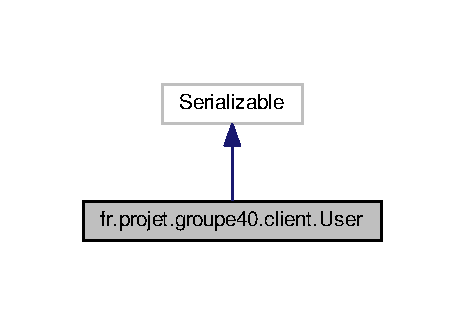
\includegraphics[width=223pt]{classfr_1_1projet_1_1groupe40_1_1client_1_1_user__inherit__graph}
\end{center}
\end{figure}


Collaboration diagram for fr.\+projet.\+groupe40.\+client.\+User\+:\nopagebreak
\begin{figure}[H]
\begin{center}
\leavevmode
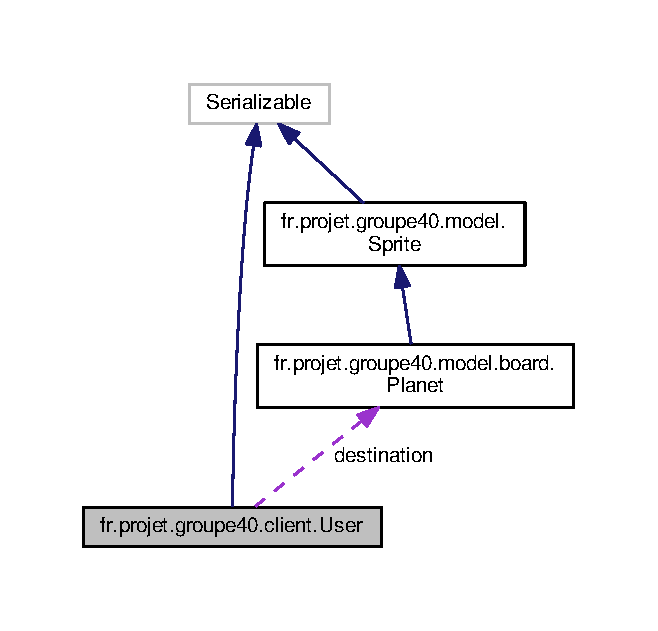
\includegraphics[width=316pt]{classfr_1_1projet_1_1groupe40_1_1client_1_1_user__coll__graph}
\end{center}
\end{figure}
\subsection*{Public Member Functions}
\begin{DoxyCompactItemize}
\item 
\hyperlink{classfr_1_1projet_1_1groupe40_1_1client_1_1_user_ad05b0747c066a5ee35cd9757c78b0e79}{User} (int faction, int id)
\item 
\hyperlink{classfr_1_1projet_1_1groupe40_1_1client_1_1_user_abb1c1439d37610e687fef97ef9739847}{User} (int faction)
\item 
\hyperlink{classfr_1_1projet_1_1groupe40_1_1client_1_1_user_abd0f6ca78045b1882f0e4f576de351ac}{User} (\hyperlink{classfr_1_1projet_1_1groupe40_1_1client_1_1_user}{User} user)
\item 
\hyperlink{classfr_1_1projet_1_1groupe40_1_1model_1_1ships_1_1_squad}{Squad} \hyperlink{classfr_1_1projet_1_1groupe40_1_1client_1_1_user_ae92f13258745de76aec592e0f86c63c6}{send\+Fleet\+AI} (\hyperlink{classfr_1_1projet_1_1groupe40_1_1model_1_1board_1_1_planet}{Planet} source, \hyperlink{classfr_1_1projet_1_1groupe40_1_1model_1_1board_1_1_planet}{Planet} destination)
\item 
boolean \hyperlink{classfr_1_1projet_1_1groupe40_1_1client_1_1_user_ad73c37bc0d6cecbd3c80bb3bb4d8abea}{has\+Lost} ()
\item 
void \hyperlink{classfr_1_1projet_1_1groupe40_1_1client_1_1_user_abefc893a751c16f2429593717fee0dda}{render\+When\+Defeat} (Graphics\+Context gc)
\item 
int \hyperlink{classfr_1_1projet_1_1groupe40_1_1client_1_1_user_a8bba484aaed66955962f9ebae579286d}{get\+Faction} ()
\item 
void \hyperlink{classfr_1_1projet_1_1groupe40_1_1client_1_1_user_a175c4059c0dd6fa229ae593de560777f}{set\+Faction} (int faction)
\item 
int \hyperlink{classfr_1_1projet_1_1groupe40_1_1client_1_1_user_a521f0939031b70091a061ba0ef6907cf}{get\+Id} ()
\item 
void \hyperlink{classfr_1_1projet_1_1groupe40_1_1client_1_1_user_aaee35ff762f9b12a3819c645c25d7dd5}{set\+Id} (int id)
\item 
int \hyperlink{classfr_1_1projet_1_1groupe40_1_1client_1_1_user_a7d0087e12b325e0d09be7e64556d3183}{get\+Percent\+\_\+of\+\_\+troups\+\_\+to\+\_\+send} ()
\item 
void \hyperlink{classfr_1_1projet_1_1groupe40_1_1client_1_1_user_a2eef817de379ad3bf873c7960df2f2cc}{set\+Percent\+\_\+of\+\_\+troups\+\_\+to\+\_\+send} (int percent\+\_\+of\+\_\+troups\+\_\+to\+\_\+send)
\item 
\hyperlink{classfr_1_1projet_1_1groupe40_1_1model_1_1board_1_1_planet}{Planet} \hyperlink{classfr_1_1projet_1_1groupe40_1_1client_1_1_user_a9e98177d60b2cde17b9b41a37ba940ed}{get\+Destination} ()
\item 
void \hyperlink{classfr_1_1projet_1_1groupe40_1_1client_1_1_user_af7251a37f51a0044001bd67e421a6688}{set\+Destination} (\hyperlink{classfr_1_1projet_1_1groupe40_1_1model_1_1board_1_1_planet}{Planet} destination)
\item 
\hyperlink{classfr_1_1projet_1_1groupe40_1_1model_1_1board_1_1_planet}{Planet} \hyperlink{classfr_1_1projet_1_1groupe40_1_1client_1_1_user_a5f6ae24ee84e918ecd49638a9c1ca340}{get\+Source} ()
\item 
void \hyperlink{classfr_1_1projet_1_1groupe40_1_1client_1_1_user_a0ce1d1c1323e06ac29b2f8a129d90762}{set\+Source} (\hyperlink{classfr_1_1projet_1_1groupe40_1_1model_1_1board_1_1_planet}{Planet} source)
\item 
boolean \hyperlink{classfr_1_1projet_1_1groupe40_1_1client_1_1_user_a6df13bfed938d9847227a61b0d8a8d3c}{is\+Lost} ()
\item 
void \hyperlink{classfr_1_1projet_1_1groupe40_1_1client_1_1_user_a408635deee87b86bdfa10835ab90ad9d}{set\+Lost} (boolean lost)
\item 
boolean \hyperlink{classfr_1_1projet_1_1groupe40_1_1client_1_1_user_a33de252fa11ff7dd91275f4f5ff1266b}{equals} (\hyperlink{classfr_1_1projet_1_1groupe40_1_1client_1_1_user}{User} u)
\end{DoxyCompactItemize}


\subsection{Constructor \& Destructor Documentation}
\mbox{\Hypertarget{classfr_1_1projet_1_1groupe40_1_1client_1_1_user_ad05b0747c066a5ee35cd9757c78b0e79}\label{classfr_1_1projet_1_1groupe40_1_1client_1_1_user_ad05b0747c066a5ee35cd9757c78b0e79}} 
\index{fr\+::projet\+::groupe40\+::client\+::\+User@{fr\+::projet\+::groupe40\+::client\+::\+User}!User@{User}}
\index{User@{User}!fr\+::projet\+::groupe40\+::client\+::\+User@{fr\+::projet\+::groupe40\+::client\+::\+User}}
\subsubsection{\texorpdfstring{User()}{User()}\hspace{0.1cm}{\footnotesize\ttfamily [1/3]}}
{\footnotesize\ttfamily fr.\+projet.\+groupe40.\+client.\+User.\+User (\begin{DoxyParamCaption}\item[{int}]{faction,  }\item[{int}]{id }\end{DoxyParamCaption})}

\mbox{\Hypertarget{classfr_1_1projet_1_1groupe40_1_1client_1_1_user_abb1c1439d37610e687fef97ef9739847}\label{classfr_1_1projet_1_1groupe40_1_1client_1_1_user_abb1c1439d37610e687fef97ef9739847}} 
\index{fr\+::projet\+::groupe40\+::client\+::\+User@{fr\+::projet\+::groupe40\+::client\+::\+User}!User@{User}}
\index{User@{User}!fr\+::projet\+::groupe40\+::client\+::\+User@{fr\+::projet\+::groupe40\+::client\+::\+User}}
\subsubsection{\texorpdfstring{User()}{User()}\hspace{0.1cm}{\footnotesize\ttfamily [2/3]}}
{\footnotesize\ttfamily fr.\+projet.\+groupe40.\+client.\+User.\+User (\begin{DoxyParamCaption}\item[{int}]{faction }\end{DoxyParamCaption})}

\mbox{\Hypertarget{classfr_1_1projet_1_1groupe40_1_1client_1_1_user_abd0f6ca78045b1882f0e4f576de351ac}\label{classfr_1_1projet_1_1groupe40_1_1client_1_1_user_abd0f6ca78045b1882f0e4f576de351ac}} 
\index{fr\+::projet\+::groupe40\+::client\+::\+User@{fr\+::projet\+::groupe40\+::client\+::\+User}!User@{User}}
\index{User@{User}!fr\+::projet\+::groupe40\+::client\+::\+User@{fr\+::projet\+::groupe40\+::client\+::\+User}}
\subsubsection{\texorpdfstring{User()}{User()}\hspace{0.1cm}{\footnotesize\ttfamily [3/3]}}
{\footnotesize\ttfamily fr.\+projet.\+groupe40.\+client.\+User.\+User (\begin{DoxyParamCaption}\item[{\hyperlink{classfr_1_1projet_1_1groupe40_1_1client_1_1_user}{User}}]{user }\end{DoxyParamCaption})}



\subsection{Member Function Documentation}
\mbox{\Hypertarget{classfr_1_1projet_1_1groupe40_1_1client_1_1_user_a33de252fa11ff7dd91275f4f5ff1266b}\label{classfr_1_1projet_1_1groupe40_1_1client_1_1_user_a33de252fa11ff7dd91275f4f5ff1266b}} 
\index{fr\+::projet\+::groupe40\+::client\+::\+User@{fr\+::projet\+::groupe40\+::client\+::\+User}!equals@{equals}}
\index{equals@{equals}!fr\+::projet\+::groupe40\+::client\+::\+User@{fr\+::projet\+::groupe40\+::client\+::\+User}}
\subsubsection{\texorpdfstring{equals()}{equals()}}
{\footnotesize\ttfamily boolean fr.\+projet.\+groupe40.\+client.\+User.\+equals (\begin{DoxyParamCaption}\item[{\hyperlink{classfr_1_1projet_1_1groupe40_1_1client_1_1_user}{User}}]{u }\end{DoxyParamCaption})}

\mbox{\Hypertarget{classfr_1_1projet_1_1groupe40_1_1client_1_1_user_a9e98177d60b2cde17b9b41a37ba940ed}\label{classfr_1_1projet_1_1groupe40_1_1client_1_1_user_a9e98177d60b2cde17b9b41a37ba940ed}} 
\index{fr\+::projet\+::groupe40\+::client\+::\+User@{fr\+::projet\+::groupe40\+::client\+::\+User}!get\+Destination@{get\+Destination}}
\index{get\+Destination@{get\+Destination}!fr\+::projet\+::groupe40\+::client\+::\+User@{fr\+::projet\+::groupe40\+::client\+::\+User}}
\subsubsection{\texorpdfstring{get\+Destination()}{getDestination()}}
{\footnotesize\ttfamily \hyperlink{classfr_1_1projet_1_1groupe40_1_1model_1_1board_1_1_planet}{Planet} fr.\+projet.\+groupe40.\+client.\+User.\+get\+Destination (\begin{DoxyParamCaption}{ }\end{DoxyParamCaption})}

\begin{DoxyReturn}{Returns}
the destination 
\end{DoxyReturn}
\mbox{\Hypertarget{classfr_1_1projet_1_1groupe40_1_1client_1_1_user_a8bba484aaed66955962f9ebae579286d}\label{classfr_1_1projet_1_1groupe40_1_1client_1_1_user_a8bba484aaed66955962f9ebae579286d}} 
\index{fr\+::projet\+::groupe40\+::client\+::\+User@{fr\+::projet\+::groupe40\+::client\+::\+User}!get\+Faction@{get\+Faction}}
\index{get\+Faction@{get\+Faction}!fr\+::projet\+::groupe40\+::client\+::\+User@{fr\+::projet\+::groupe40\+::client\+::\+User}}
\subsubsection{\texorpdfstring{get\+Faction()}{getFaction()}}
{\footnotesize\ttfamily int fr.\+projet.\+groupe40.\+client.\+User.\+get\+Faction (\begin{DoxyParamCaption}{ }\end{DoxyParamCaption})}

\mbox{\Hypertarget{classfr_1_1projet_1_1groupe40_1_1client_1_1_user_a521f0939031b70091a061ba0ef6907cf}\label{classfr_1_1projet_1_1groupe40_1_1client_1_1_user_a521f0939031b70091a061ba0ef6907cf}} 
\index{fr\+::projet\+::groupe40\+::client\+::\+User@{fr\+::projet\+::groupe40\+::client\+::\+User}!get\+Id@{get\+Id}}
\index{get\+Id@{get\+Id}!fr\+::projet\+::groupe40\+::client\+::\+User@{fr\+::projet\+::groupe40\+::client\+::\+User}}
\subsubsection{\texorpdfstring{get\+Id()}{getId()}}
{\footnotesize\ttfamily int fr.\+projet.\+groupe40.\+client.\+User.\+get\+Id (\begin{DoxyParamCaption}{ }\end{DoxyParamCaption})}

\mbox{\Hypertarget{classfr_1_1projet_1_1groupe40_1_1client_1_1_user_a7d0087e12b325e0d09be7e64556d3183}\label{classfr_1_1projet_1_1groupe40_1_1client_1_1_user_a7d0087e12b325e0d09be7e64556d3183}} 
\index{fr\+::projet\+::groupe40\+::client\+::\+User@{fr\+::projet\+::groupe40\+::client\+::\+User}!get\+Percent\+\_\+of\+\_\+troups\+\_\+to\+\_\+send@{get\+Percent\+\_\+of\+\_\+troups\+\_\+to\+\_\+send}}
\index{get\+Percent\+\_\+of\+\_\+troups\+\_\+to\+\_\+send@{get\+Percent\+\_\+of\+\_\+troups\+\_\+to\+\_\+send}!fr\+::projet\+::groupe40\+::client\+::\+User@{fr\+::projet\+::groupe40\+::client\+::\+User}}
\subsubsection{\texorpdfstring{get\+Percent\+\_\+of\+\_\+troups\+\_\+to\+\_\+send()}{getPercent\_of\_troups\_to\_send()}}
{\footnotesize\ttfamily int fr.\+projet.\+groupe40.\+client.\+User.\+get\+Percent\+\_\+of\+\_\+troups\+\_\+to\+\_\+send (\begin{DoxyParamCaption}{ }\end{DoxyParamCaption})}

\begin{DoxyReturn}{Returns}
the percent\+\_\+of\+\_\+troups\+\_\+to\+\_\+send 
\end{DoxyReturn}
\mbox{\Hypertarget{classfr_1_1projet_1_1groupe40_1_1client_1_1_user_a5f6ae24ee84e918ecd49638a9c1ca340}\label{classfr_1_1projet_1_1groupe40_1_1client_1_1_user_a5f6ae24ee84e918ecd49638a9c1ca340}} 
\index{fr\+::projet\+::groupe40\+::client\+::\+User@{fr\+::projet\+::groupe40\+::client\+::\+User}!get\+Source@{get\+Source}}
\index{get\+Source@{get\+Source}!fr\+::projet\+::groupe40\+::client\+::\+User@{fr\+::projet\+::groupe40\+::client\+::\+User}}
\subsubsection{\texorpdfstring{get\+Source()}{getSource()}}
{\footnotesize\ttfamily \hyperlink{classfr_1_1projet_1_1groupe40_1_1model_1_1board_1_1_planet}{Planet} fr.\+projet.\+groupe40.\+client.\+User.\+get\+Source (\begin{DoxyParamCaption}{ }\end{DoxyParamCaption})}

\begin{DoxyReturn}{Returns}
the source 
\end{DoxyReturn}
\mbox{\Hypertarget{classfr_1_1projet_1_1groupe40_1_1client_1_1_user_ad73c37bc0d6cecbd3c80bb3bb4d8abea}\label{classfr_1_1projet_1_1groupe40_1_1client_1_1_user_ad73c37bc0d6cecbd3c80bb3bb4d8abea}} 
\index{fr\+::projet\+::groupe40\+::client\+::\+User@{fr\+::projet\+::groupe40\+::client\+::\+User}!has\+Lost@{has\+Lost}}
\index{has\+Lost@{has\+Lost}!fr\+::projet\+::groupe40\+::client\+::\+User@{fr\+::projet\+::groupe40\+::client\+::\+User}}
\subsubsection{\texorpdfstring{has\+Lost()}{hasLost()}}
{\footnotesize\ttfamily boolean fr.\+projet.\+groupe40.\+client.\+User.\+has\+Lost (\begin{DoxyParamCaption}{ }\end{DoxyParamCaption})}

\mbox{\Hypertarget{classfr_1_1projet_1_1groupe40_1_1client_1_1_user_a6df13bfed938d9847227a61b0d8a8d3c}\label{classfr_1_1projet_1_1groupe40_1_1client_1_1_user_a6df13bfed938d9847227a61b0d8a8d3c}} 
\index{fr\+::projet\+::groupe40\+::client\+::\+User@{fr\+::projet\+::groupe40\+::client\+::\+User}!is\+Lost@{is\+Lost}}
\index{is\+Lost@{is\+Lost}!fr\+::projet\+::groupe40\+::client\+::\+User@{fr\+::projet\+::groupe40\+::client\+::\+User}}
\subsubsection{\texorpdfstring{is\+Lost()}{isLost()}}
{\footnotesize\ttfamily boolean fr.\+projet.\+groupe40.\+client.\+User.\+is\+Lost (\begin{DoxyParamCaption}{ }\end{DoxyParamCaption})}

\mbox{\Hypertarget{classfr_1_1projet_1_1groupe40_1_1client_1_1_user_abefc893a751c16f2429593717fee0dda}\label{classfr_1_1projet_1_1groupe40_1_1client_1_1_user_abefc893a751c16f2429593717fee0dda}} 
\index{fr\+::projet\+::groupe40\+::client\+::\+User@{fr\+::projet\+::groupe40\+::client\+::\+User}!render\+When\+Defeat@{render\+When\+Defeat}}
\index{render\+When\+Defeat@{render\+When\+Defeat}!fr\+::projet\+::groupe40\+::client\+::\+User@{fr\+::projet\+::groupe40\+::client\+::\+User}}
\subsubsection{\texorpdfstring{render\+When\+Defeat()}{renderWhenDefeat()}}
{\footnotesize\ttfamily void fr.\+projet.\+groupe40.\+client.\+User.\+render\+When\+Defeat (\begin{DoxyParamCaption}\item[{Graphics\+Context}]{gc }\end{DoxyParamCaption})}

\mbox{\Hypertarget{classfr_1_1projet_1_1groupe40_1_1client_1_1_user_ae92f13258745de76aec592e0f86c63c6}\label{classfr_1_1projet_1_1groupe40_1_1client_1_1_user_ae92f13258745de76aec592e0f86c63c6}} 
\index{fr\+::projet\+::groupe40\+::client\+::\+User@{fr\+::projet\+::groupe40\+::client\+::\+User}!send\+Fleet\+AI@{send\+Fleet\+AI}}
\index{send\+Fleet\+AI@{send\+Fleet\+AI}!fr\+::projet\+::groupe40\+::client\+::\+User@{fr\+::projet\+::groupe40\+::client\+::\+User}}
\subsubsection{\texorpdfstring{send\+Fleet\+A\+I()}{sendFleetAI()}}
{\footnotesize\ttfamily \hyperlink{classfr_1_1projet_1_1groupe40_1_1model_1_1ships_1_1_squad}{Squad} fr.\+projet.\+groupe40.\+client.\+User.\+send\+Fleet\+AI (\begin{DoxyParamCaption}\item[{\hyperlink{classfr_1_1projet_1_1groupe40_1_1model_1_1board_1_1_planet}{Planet}}]{source,  }\item[{\hyperlink{classfr_1_1projet_1_1groupe40_1_1model_1_1board_1_1_planet}{Planet}}]{destination }\end{DoxyParamCaption})}

AI handler \mbox{\Hypertarget{classfr_1_1projet_1_1groupe40_1_1client_1_1_user_af7251a37f51a0044001bd67e421a6688}\label{classfr_1_1projet_1_1groupe40_1_1client_1_1_user_af7251a37f51a0044001bd67e421a6688}} 
\index{fr\+::projet\+::groupe40\+::client\+::\+User@{fr\+::projet\+::groupe40\+::client\+::\+User}!set\+Destination@{set\+Destination}}
\index{set\+Destination@{set\+Destination}!fr\+::projet\+::groupe40\+::client\+::\+User@{fr\+::projet\+::groupe40\+::client\+::\+User}}
\subsubsection{\texorpdfstring{set\+Destination()}{setDestination()}}
{\footnotesize\ttfamily void fr.\+projet.\+groupe40.\+client.\+User.\+set\+Destination (\begin{DoxyParamCaption}\item[{\hyperlink{classfr_1_1projet_1_1groupe40_1_1model_1_1board_1_1_planet}{Planet}}]{destination }\end{DoxyParamCaption})}


\begin{DoxyParams}{Parameters}
{\em destination} & the destination to set \\
\hline
\end{DoxyParams}
\mbox{\Hypertarget{classfr_1_1projet_1_1groupe40_1_1client_1_1_user_a175c4059c0dd6fa229ae593de560777f}\label{classfr_1_1projet_1_1groupe40_1_1client_1_1_user_a175c4059c0dd6fa229ae593de560777f}} 
\index{fr\+::projet\+::groupe40\+::client\+::\+User@{fr\+::projet\+::groupe40\+::client\+::\+User}!set\+Faction@{set\+Faction}}
\index{set\+Faction@{set\+Faction}!fr\+::projet\+::groupe40\+::client\+::\+User@{fr\+::projet\+::groupe40\+::client\+::\+User}}
\subsubsection{\texorpdfstring{set\+Faction()}{setFaction()}}
{\footnotesize\ttfamily void fr.\+projet.\+groupe40.\+client.\+User.\+set\+Faction (\begin{DoxyParamCaption}\item[{int}]{faction }\end{DoxyParamCaption})}

\mbox{\Hypertarget{classfr_1_1projet_1_1groupe40_1_1client_1_1_user_aaee35ff762f9b12a3819c645c25d7dd5}\label{classfr_1_1projet_1_1groupe40_1_1client_1_1_user_aaee35ff762f9b12a3819c645c25d7dd5}} 
\index{fr\+::projet\+::groupe40\+::client\+::\+User@{fr\+::projet\+::groupe40\+::client\+::\+User}!set\+Id@{set\+Id}}
\index{set\+Id@{set\+Id}!fr\+::projet\+::groupe40\+::client\+::\+User@{fr\+::projet\+::groupe40\+::client\+::\+User}}
\subsubsection{\texorpdfstring{set\+Id()}{setId()}}
{\footnotesize\ttfamily void fr.\+projet.\+groupe40.\+client.\+User.\+set\+Id (\begin{DoxyParamCaption}\item[{int}]{id }\end{DoxyParamCaption})}

\mbox{\Hypertarget{classfr_1_1projet_1_1groupe40_1_1client_1_1_user_a408635deee87b86bdfa10835ab90ad9d}\label{classfr_1_1projet_1_1groupe40_1_1client_1_1_user_a408635deee87b86bdfa10835ab90ad9d}} 
\index{fr\+::projet\+::groupe40\+::client\+::\+User@{fr\+::projet\+::groupe40\+::client\+::\+User}!set\+Lost@{set\+Lost}}
\index{set\+Lost@{set\+Lost}!fr\+::projet\+::groupe40\+::client\+::\+User@{fr\+::projet\+::groupe40\+::client\+::\+User}}
\subsubsection{\texorpdfstring{set\+Lost()}{setLost()}}
{\footnotesize\ttfamily void fr.\+projet.\+groupe40.\+client.\+User.\+set\+Lost (\begin{DoxyParamCaption}\item[{boolean}]{lost }\end{DoxyParamCaption})}

\mbox{\Hypertarget{classfr_1_1projet_1_1groupe40_1_1client_1_1_user_a2eef817de379ad3bf873c7960df2f2cc}\label{classfr_1_1projet_1_1groupe40_1_1client_1_1_user_a2eef817de379ad3bf873c7960df2f2cc}} 
\index{fr\+::projet\+::groupe40\+::client\+::\+User@{fr\+::projet\+::groupe40\+::client\+::\+User}!set\+Percent\+\_\+of\+\_\+troups\+\_\+to\+\_\+send@{set\+Percent\+\_\+of\+\_\+troups\+\_\+to\+\_\+send}}
\index{set\+Percent\+\_\+of\+\_\+troups\+\_\+to\+\_\+send@{set\+Percent\+\_\+of\+\_\+troups\+\_\+to\+\_\+send}!fr\+::projet\+::groupe40\+::client\+::\+User@{fr\+::projet\+::groupe40\+::client\+::\+User}}
\subsubsection{\texorpdfstring{set\+Percent\+\_\+of\+\_\+troups\+\_\+to\+\_\+send()}{setPercent\_of\_troups\_to\_send()}}
{\footnotesize\ttfamily void fr.\+projet.\+groupe40.\+client.\+User.\+set\+Percent\+\_\+of\+\_\+troups\+\_\+to\+\_\+send (\begin{DoxyParamCaption}\item[{int}]{percent\+\_\+of\+\_\+troups\+\_\+to\+\_\+send }\end{DoxyParamCaption})}


\begin{DoxyParams}{Parameters}
{\em percent\+\_\+of\+\_\+troups\+\_\+to\+\_\+send} & the percent\+\_\+of\+\_\+troups\+\_\+to\+\_\+send to set \\
\hline
\end{DoxyParams}
\mbox{\Hypertarget{classfr_1_1projet_1_1groupe40_1_1client_1_1_user_a0ce1d1c1323e06ac29b2f8a129d90762}\label{classfr_1_1projet_1_1groupe40_1_1client_1_1_user_a0ce1d1c1323e06ac29b2f8a129d90762}} 
\index{fr\+::projet\+::groupe40\+::client\+::\+User@{fr\+::projet\+::groupe40\+::client\+::\+User}!set\+Source@{set\+Source}}
\index{set\+Source@{set\+Source}!fr\+::projet\+::groupe40\+::client\+::\+User@{fr\+::projet\+::groupe40\+::client\+::\+User}}
\subsubsection{\texorpdfstring{set\+Source()}{setSource()}}
{\footnotesize\ttfamily void fr.\+projet.\+groupe40.\+client.\+User.\+set\+Source (\begin{DoxyParamCaption}\item[{\hyperlink{classfr_1_1projet_1_1groupe40_1_1model_1_1board_1_1_planet}{Planet}}]{source }\end{DoxyParamCaption})}


\begin{DoxyParams}{Parameters}
{\em source} & the source to set \\
\hline
\end{DoxyParams}


The documentation for this class was generated from the following file\+:\begin{DoxyCompactItemize}
\item 
src/fr/projet/groupe40/client/\hyperlink{_user_8java}{User.\+java}\end{DoxyCompactItemize}

\chapter{File Documentation}
\hypertarget{_interaction_handler_8java}{}\section{src/fr/projet/groupe40/client/handler/\+Interaction\+Handler.java File Reference}
\label{_interaction_handler_8java}\index{src/fr/projet/groupe40/client/handler/\+Interaction\+Handler.\+java@{src/fr/projet/groupe40/client/handler/\+Interaction\+Handler.\+java}}
\subsection*{Classes}
\begin{DoxyCompactItemize}
\item 
class \hyperlink{classfr_1_1projet_1_1groupe40_1_1client_1_1handler_1_1_interaction_handler}{fr.\+projet.\+groupe40.\+client.\+handler.\+Interaction\+Handler}
\end{DoxyCompactItemize}
\subsection*{Packages}
\begin{DoxyCompactItemize}
\item 
package \hyperlink{namespacefr_1_1projet_1_1groupe40_1_1client_1_1handler}{fr.\+projet.\+groupe40.\+client.\+handler}
\end{DoxyCompactItemize}

\hypertarget{_keyboard_handler_8java}{}\section{src/fr/projet/groupe40/client/handler/\+Keyboard\+Handler.java File Reference}
\label{_keyboard_handler_8java}\index{src/fr/projet/groupe40/client/handler/\+Keyboard\+Handler.\+java@{src/fr/projet/groupe40/client/handler/\+Keyboard\+Handler.\+java}}
\subsection*{Classes}
\begin{DoxyCompactItemize}
\item 
class \hyperlink{classfr_1_1projet_1_1groupe40_1_1client_1_1handler_1_1_keyboard_handler}{fr.\+projet.\+groupe40.\+client.\+handler.\+Keyboard\+Handler}
\end{DoxyCompactItemize}
\subsection*{Packages}
\begin{DoxyCompactItemize}
\item 
package \hyperlink{namespacefr_1_1projet_1_1groupe40_1_1client_1_1handler}{fr.\+projet.\+groupe40.\+client.\+handler}
\end{DoxyCompactItemize}

\hypertarget{_mouse_handler_8java}{}\section{src/fr/projet/groupe40/client/handler/\+Mouse\+Handler.java File Reference}
\label{_mouse_handler_8java}\index{src/fr/projet/groupe40/client/handler/\+Mouse\+Handler.\+java@{src/fr/projet/groupe40/client/handler/\+Mouse\+Handler.\+java}}
\subsection*{Classes}
\begin{DoxyCompactItemize}
\item 
class \hyperlink{classfr_1_1projet_1_1groupe40_1_1client_1_1handler_1_1_mouse_handler}{fr.\+projet.\+groupe40.\+client.\+handler.\+Mouse\+Handler}
\end{DoxyCompactItemize}
\subsection*{Packages}
\begin{DoxyCompactItemize}
\item 
package \hyperlink{namespacefr_1_1projet_1_1groupe40_1_1client_1_1handler}{fr.\+projet.\+groupe40.\+client.\+handler}
\end{DoxyCompactItemize}

\hypertarget{_user_8java}{}\section{src/fr/projet/groupe40/client/\+User.java File Reference}
\label{_user_8java}\index{src/fr/projet/groupe40/client/\+User.\+java@{src/fr/projet/groupe40/client/\+User.\+java}}
\subsection*{Classes}
\begin{DoxyCompactItemize}
\item 
class \hyperlink{classfr_1_1projet_1_1groupe40_1_1client_1_1_user}{fr.\+projet.\+groupe40.\+client.\+User}
\end{DoxyCompactItemize}
\subsection*{Packages}
\begin{DoxyCompactItemize}
\item 
package \hyperlink{namespacefr_1_1projet_1_1groupe40_1_1client}{fr.\+projet.\+groupe40.\+client}
\end{DoxyCompactItemize}

\hypertarget{_events_8java}{}\section{src/fr/projet/groupe40/events/\+Events.java File Reference}
\label{_events_8java}\index{src/fr/projet/groupe40/events/\+Events.\+java@{src/fr/projet/groupe40/events/\+Events.\+java}}
\subsection*{Classes}
\begin{DoxyCompactItemize}
\item 
class \hyperlink{classfr_1_1projet_1_1groupe40_1_1events_1_1_events}{fr.\+projet.\+groupe40.\+events.\+Events}
\end{DoxyCompactItemize}
\subsection*{Packages}
\begin{DoxyCompactItemize}
\item 
package \hyperlink{namespacefr_1_1projet_1_1groupe40_1_1events}{fr.\+projet.\+groupe40.\+events}
\end{DoxyCompactItemize}

\hypertarget{_pirate_assault_8java}{}\section{src/fr/projet/groupe40/events/\+Pirate\+Assault.java File Reference}
\label{_pirate_assault_8java}\index{src/fr/projet/groupe40/events/\+Pirate\+Assault.\+java@{src/fr/projet/groupe40/events/\+Pirate\+Assault.\+java}}
\subsection*{Classes}
\begin{DoxyCompactItemize}
\item 
class \hyperlink{classfr_1_1projet_1_1groupe40_1_1events_1_1_pirate_assault}{fr.\+projet.\+groupe40.\+events.\+Pirate\+Assault}
\end{DoxyCompactItemize}
\subsection*{Packages}
\begin{DoxyCompactItemize}
\item 
package \hyperlink{namespacefr_1_1projet_1_1groupe40_1_1events}{fr.\+projet.\+groupe40.\+events}
\end{DoxyCompactItemize}

\hypertarget{_data_serializer_8java}{}\section{src/fr/projet/groupe40/file/\+Data\+Serializer.java File Reference}
\label{_data_serializer_8java}\index{src/fr/projet/groupe40/file/\+Data\+Serializer.\+java@{src/fr/projet/groupe40/file/\+Data\+Serializer.\+java}}
\subsection*{Classes}
\begin{DoxyCompactItemize}
\item 
class \hyperlink{classfr_1_1projet_1_1groupe40_1_1file_1_1_data_serializer}{fr.\+projet.\+groupe40.\+file.\+Data\+Serializer}
\end{DoxyCompactItemize}
\subsection*{Packages}
\begin{DoxyCompactItemize}
\item 
package \hyperlink{namespacefr_1_1projet_1_1groupe40_1_1file}{fr.\+projet.\+groupe40.\+file}
\end{DoxyCompactItemize}

\hypertarget{_game_8java}{}\section{src/fr/projet/groupe40/\+Game.java File Reference}
\label{_game_8java}\index{src/fr/projet/groupe40/\+Game.\+java@{src/fr/projet/groupe40/\+Game.\+java}}
\subsection*{Classes}
\begin{DoxyCompactItemize}
\item 
class \hyperlink{classfr_1_1projet_1_1groupe40_1_1_game}{fr.\+projet.\+groupe40.\+Game}
\end{DoxyCompactItemize}
\subsection*{Packages}
\begin{DoxyCompactItemize}
\item 
package \hyperlink{namespacefr_1_1projet_1_1groupe40}{fr.\+projet.\+groupe40}
\end{DoxyCompactItemize}

\hypertarget{_galaxy_8java}{}\section{src/fr/projet/groupe40/model/board/\+Galaxy.java File Reference}
\label{_galaxy_8java}\index{src/fr/projet/groupe40/model/board/\+Galaxy.\+java@{src/fr/projet/groupe40/model/board/\+Galaxy.\+java}}
\subsection*{Classes}
\begin{DoxyCompactItemize}
\item 
class \hyperlink{classfr_1_1projet_1_1groupe40_1_1model_1_1board_1_1_galaxy}{fr.\+projet.\+groupe40.\+model.\+board.\+Galaxy}
\end{DoxyCompactItemize}
\subsection*{Packages}
\begin{DoxyCompactItemize}
\item 
package \hyperlink{namespacefr_1_1projet_1_1groupe40_1_1model_1_1board}{fr.\+projet.\+groupe40.\+model.\+board}
\end{DoxyCompactItemize}

\hypertarget{_planet_8java}{}\section{src/fr/projet/groupe40/model/board/\+Planet.java File Reference}
\label{_planet_8java}\index{src/fr/projet/groupe40/model/board/\+Planet.\+java@{src/fr/projet/groupe40/model/board/\+Planet.\+java}}
\subsection*{Classes}
\begin{DoxyCompactItemize}
\item 
class \hyperlink{classfr_1_1projet_1_1groupe40_1_1model_1_1board_1_1_planet}{fr.\+projet.\+groupe40.\+model.\+board.\+Planet}
\end{DoxyCompactItemize}
\subsection*{Packages}
\begin{DoxyCompactItemize}
\item 
package \hyperlink{namespacefr_1_1projet_1_1groupe40_1_1model_1_1board}{fr.\+projet.\+groupe40.\+model.\+board}
\end{DoxyCompactItemize}

\hypertarget{_round_planet_8java}{}\section{src/fr/projet/groupe40/model/planets/\+Round\+Planet.java File Reference}
\label{_round_planet_8java}\index{src/fr/projet/groupe40/model/planets/\+Round\+Planet.\+java@{src/fr/projet/groupe40/model/planets/\+Round\+Planet.\+java}}
\subsection*{Classes}
\begin{DoxyCompactItemize}
\item 
class \hyperlink{classfr_1_1projet_1_1groupe40_1_1model_1_1planets_1_1_round_planet}{fr.\+projet.\+groupe40.\+model.\+planets.\+Round\+Planet}
\end{DoxyCompactItemize}
\subsection*{Packages}
\begin{DoxyCompactItemize}
\item 
package \hyperlink{namespacefr_1_1projet_1_1groupe40_1_1model_1_1planets}{fr.\+projet.\+groupe40.\+model.\+planets}
\end{DoxyCompactItemize}

\hypertarget{_ship_8java}{}\section{src/fr/projet/groupe40/model/ships/\+Ship.java File Reference}
\label{_ship_8java}\index{src/fr/projet/groupe40/model/ships/\+Ship.\+java@{src/fr/projet/groupe40/model/ships/\+Ship.\+java}}
\subsection*{Classes}
\begin{DoxyCompactItemize}
\item 
class \hyperlink{classfr_1_1projet_1_1groupe40_1_1model_1_1ships_1_1_ship}{fr.\+projet.\+groupe40.\+model.\+ships.\+Ship}
\end{DoxyCompactItemize}
\subsection*{Packages}
\begin{DoxyCompactItemize}
\item 
package \hyperlink{namespacefr_1_1projet_1_1groupe40_1_1model_1_1ships}{fr.\+projet.\+groupe40.\+model.\+ships}
\end{DoxyCompactItemize}

\hypertarget{_squad_8java}{}\section{src/fr/projet/groupe40/model/ships/\+Squad.java File Reference}
\label{_squad_8java}\index{src/fr/projet/groupe40/model/ships/\+Squad.\+java@{src/fr/projet/groupe40/model/ships/\+Squad.\+java}}
\subsection*{Classes}
\begin{DoxyCompactItemize}
\item 
class \hyperlink{classfr_1_1projet_1_1groupe40_1_1model_1_1ships_1_1_squad}{fr.\+projet.\+groupe40.\+model.\+ships.\+Squad}
\end{DoxyCompactItemize}
\subsection*{Packages}
\begin{DoxyCompactItemize}
\item 
package \hyperlink{namespacefr_1_1projet_1_1groupe40_1_1model_1_1ships}{fr.\+projet.\+groupe40.\+model.\+ships}
\end{DoxyCompactItemize}

\hypertarget{_sprite_8java}{}\section{src/fr/projet/groupe40/model/\+Sprite.java File Reference}
\label{_sprite_8java}\index{src/fr/projet/groupe40/model/\+Sprite.\+java@{src/fr/projet/groupe40/model/\+Sprite.\+java}}
\subsection*{Classes}
\begin{DoxyCompactItemize}
\item 
class \hyperlink{classfr_1_1projet_1_1groupe40_1_1model_1_1_sprite}{fr.\+projet.\+groupe40.\+model.\+Sprite}
\end{DoxyCompactItemize}
\subsection*{Packages}
\begin{DoxyCompactItemize}
\item 
package \hyperlink{namespacefr_1_1projet_1_1groupe40_1_1model}{fr.\+projet.\+groupe40.\+model}
\end{DoxyCompactItemize}

\hypertarget{_constantes_8java}{}\section{src/fr/projet/groupe40/util/\+Constantes.java File Reference}
\label{_constantes_8java}\index{src/fr/projet/groupe40/util/\+Constantes.\+java@{src/fr/projet/groupe40/util/\+Constantes.\+java}}
\subsection*{Classes}
\begin{DoxyCompactItemize}
\item 
class \hyperlink{classfr_1_1projet_1_1groupe40_1_1util_1_1_constantes}{fr.\+projet.\+groupe40.\+util.\+Constantes}
\end{DoxyCompactItemize}
\subsection*{Packages}
\begin{DoxyCompactItemize}
\item 
package \hyperlink{namespacefr_1_1projet_1_1groupe40_1_1util}{fr.\+projet.\+groupe40.\+util}
\end{DoxyCompactItemize}

\hypertarget{_loading_screen_8java}{}\section{src/fr/projet/groupe40/window/\+Loading\+Screen.java File Reference}
\label{_loading_screen_8java}\index{src/fr/projet/groupe40/window/\+Loading\+Screen.\+java@{src/fr/projet/groupe40/window/\+Loading\+Screen.\+java}}
\subsection*{Classes}
\begin{DoxyCompactItemize}
\item 
class \hyperlink{classfr_1_1projet_1_1groupe40_1_1window_1_1_loading_screen}{fr.\+projet.\+groupe40.\+window.\+Loading\+Screen}
\end{DoxyCompactItemize}
\subsection*{Packages}
\begin{DoxyCompactItemize}
\item 
package \hyperlink{namespacefr_1_1projet_1_1groupe40_1_1window}{fr.\+projet.\+groupe40.\+window}
\end{DoxyCompactItemize}

\hypertarget{_main_menu_8java}{}\section{src/fr/projet/groupe40/window/\+Main\+Menu.java File Reference}
\label{_main_menu_8java}\index{src/fr/projet/groupe40/window/\+Main\+Menu.\+java@{src/fr/projet/groupe40/window/\+Main\+Menu.\+java}}
\subsection*{Classes}
\begin{DoxyCompactItemize}
\item 
class \hyperlink{classfr_1_1projet_1_1groupe40_1_1window_1_1_main_menu}{fr.\+projet.\+groupe40.\+window.\+Main\+Menu}
\end{DoxyCompactItemize}
\subsection*{Packages}
\begin{DoxyCompactItemize}
\item 
package \hyperlink{namespacefr_1_1projet_1_1groupe40_1_1window}{fr.\+projet.\+groupe40.\+window}
\end{DoxyCompactItemize}

\hypertarget{_settings_menu_8java}{}\section{src/fr/projet/groupe40/window/\+Settings\+Menu.java File Reference}
\label{_settings_menu_8java}\index{src/fr/projet/groupe40/window/\+Settings\+Menu.\+java@{src/fr/projet/groupe40/window/\+Settings\+Menu.\+java}}
\subsection*{Classes}
\begin{DoxyCompactItemize}
\item 
class \hyperlink{classfr_1_1projet_1_1groupe40_1_1window_1_1_settings_menu}{fr.\+projet.\+groupe40.\+window.\+Settings\+Menu}
\end{DoxyCompactItemize}
\subsection*{Packages}
\begin{DoxyCompactItemize}
\item 
package \hyperlink{namespacefr_1_1projet_1_1groupe40_1_1window}{fr.\+projet.\+groupe40.\+window}
\end{DoxyCompactItemize}

%--- End generated contents ---

% Index
\backmatter
\newpage
\phantomsection
\clearemptydoublepage
\addcontentsline{toc}{chapter}{Index}
\printindex

\end{document}
